%----------------------------------------------------------------
%----------------------------------------------------------------
\section{Introduction}
\label{sec:Introduction}
%----------------------------------------------------------------
%----------------------------------------------------------------
The Florida Bay Assessment Model (BAM) is a 'basins' hydrological model of Florida Bay.  It is mass-conservative and explicitly designed to assess water levels and salinities in 54 idealized basins representing Florida Bay.  Basins are separated and connected by shoals, thereby the model conforms to a linked-node network hierarchy with basins as nodes and shoals as links.  Interbasin fluxes are driven by hydraulic gradients developed across the shoals in response to water level elevations and are modeled with depth integrated velocity based on frictional flow from Manning's equation.  

Each basin is forced with rainfall and evaporation.  Basins on the Gulf of Mexico and Atlantic Ocean boundaries are also forced across the appropriate shoals with sea levels consisting of tidal variations and sea level changes.  Coastal basins along the Everglades are forced with water levels determined from the Everglades Depth Estimation Network (EDEN) \citep{Telis2014} with the shoal properties (length, width, depth) calibrated to match aggregate runoff from the FATHOM model \citep{Cosby2010}.

BAM can be considered a derivative work from FATHOM since it employs the same basic physical and domain representations, however, it is significantly different in several aspects.  First, BAM uses contemporary, high-quality, high-temporal density observational data to drive model inputs and boundaries.  These environmental forcings leverage the wealth of meteorological and hydrographic observations available from the Marine Monitoring Network administered by Everglades National Park.  Tidal data are computed from local NOAA subordinate tide stations within Florida Bay containing all astronomical forcings including intrannual variations.  The reliance on high-quality, nearly continuous observational data to drive model inputs is a particular strength of BAM.

Second, BAM is pure Python.  While this imposes an operational constraint since model runtimes are slower than a compiled binary image, it affords several advantages:

\renewcommand{\labelitemi}{\textendash}
\begin{itemize}  
  \itemsep-8pt
  \item Object oriented code facilitates clarity, scalability, extensibility and developer collaboration with modern programming language dictums.
  \item Adherence to modern programming standards and naming conventions results in code that is human readable and understandable, reducing the potential for software errors. 
  \item Python dictionaries and native data containers simplify and clarify the processing of model data and objects. 
  \item Cross-platform support.  Any platform that runs Python can run BAM. 
  \item No binaries and no dependence on special compilers or licensed third-party libraries. 
\end{itemize}

Third, BAM outputs are not limited to specific time intervals, the output interval is user-controllable.  Fourth, all BAM inputs/outputs are contained in ASCII comma delimited files imposing a uniform and accessible standard for model I/O enabling the evaluation of alternative scenarios in a straightforward manner.  Fifth, the graphical user interface is designed to allow interaction and querying of model results and parameters. Each basin and shoal in the model is accessible with a mouse click on the map, or from a list box.  Integrated plotting facilities allow the comparison of model outputs from different runs.  Sixth, the GUI is not required.  BAM can be run in text-mode inside a terminal and is therefore easily controlled in batch mode by shell or other scripts. Seventh, all model controls are exposed through the command line interface which applies whether the GUI is used or not. 

Lastly, BAM is open-source.  This fosters transparency, allows community development, and empowers the individual to adjust and change any aspect of the model to suit their needs or conceptualizations. 


%----------------------------------------------------------------
\subsection{Limitations}
\label{sec:Limitations}
%----------------------------------------------------------------

The physical basis is interbasin Mannings flow over shoals with conservation of mass.  The simplified physical basis imposes several restrictions:

\begin{enumerate}
  \itemsep-8pt
  \item No wave propagation, stage/volume changes are instantaneous.
  \item No diffusion/mixing, concentration equilibriums are instantaneous.
  \item Mannings flow over deep or narrow shoals is not justifiable.
  \item Water levels are not geodetic, but anomalies with respect to zero shoal depth. 
  \item Geomorphic bank and shoal changes over time are ignored.
\end{enumerate}

\vspace{12pt}
\noindent The representation of basins, shoals and forcings is incomplete:

\begin{enumerate}
  \itemsep-8pt
  \item There are shoals with missing channels. For example, the Florida Keys are largely considered flow barriers, ignoring many channels.
  \item Evaporation is a single daily timeseries applied to the entire domain.
  \item Rainfall is a sparse set of daily timeseries.
\end{enumerate}


%----------------------------------------------------------------
%----------------------------------------------------------------
\clearpage 
\section{Model Domain}
\label{sec:Model Domain}
%----------------------------------------------------------------
%----------------------------------------------------------------
BAM decomposes Florida Bay into 54 basins based on the geomorphology of the mangroves, buttonwood banks, and shoals separating individual basins (figure \ref{fig:BAM Domain}).  Basin bathymetry is partitioned into 10 depth classes in 0.305 m (1 ft) increments following \citet{Cosby2010}.  There are 410 shoals linking the basins each characterized with a shoal width, land length (zero depth), and submerged lengths partitioned into the same 10 depth classes as the basins. Each shoal also has a Manning's friction coefficient applied over the shoal width, so that the shoal width is parallel to the interbasin flow path while the shoal lengths are perpendicular to the flow path. 

Shoal data are derived from the work of \citet{Cosby2010}, however a review of the shoals bordering domain boundaries with the Florida Keys and Everglades identified numerous deficiencies ignoring well-established flow paths between the boundaries and model basins.  These shoals were adjusted and calibrated to produce water level dynamics inside the appropriate basins consistent with observed water level data. 

%~~~~~~~~~~~~~~~~~~~~~~~~~~~~~~~~~~~~~~~~~
\begin{figure}[H]
  \floatbox[{ \capbeside\thisfloatsetup{ capbesideposition = {right, center},
                                          capbesidewidth = 4cm } }]
  {figure}[\FBwidth]
  {
    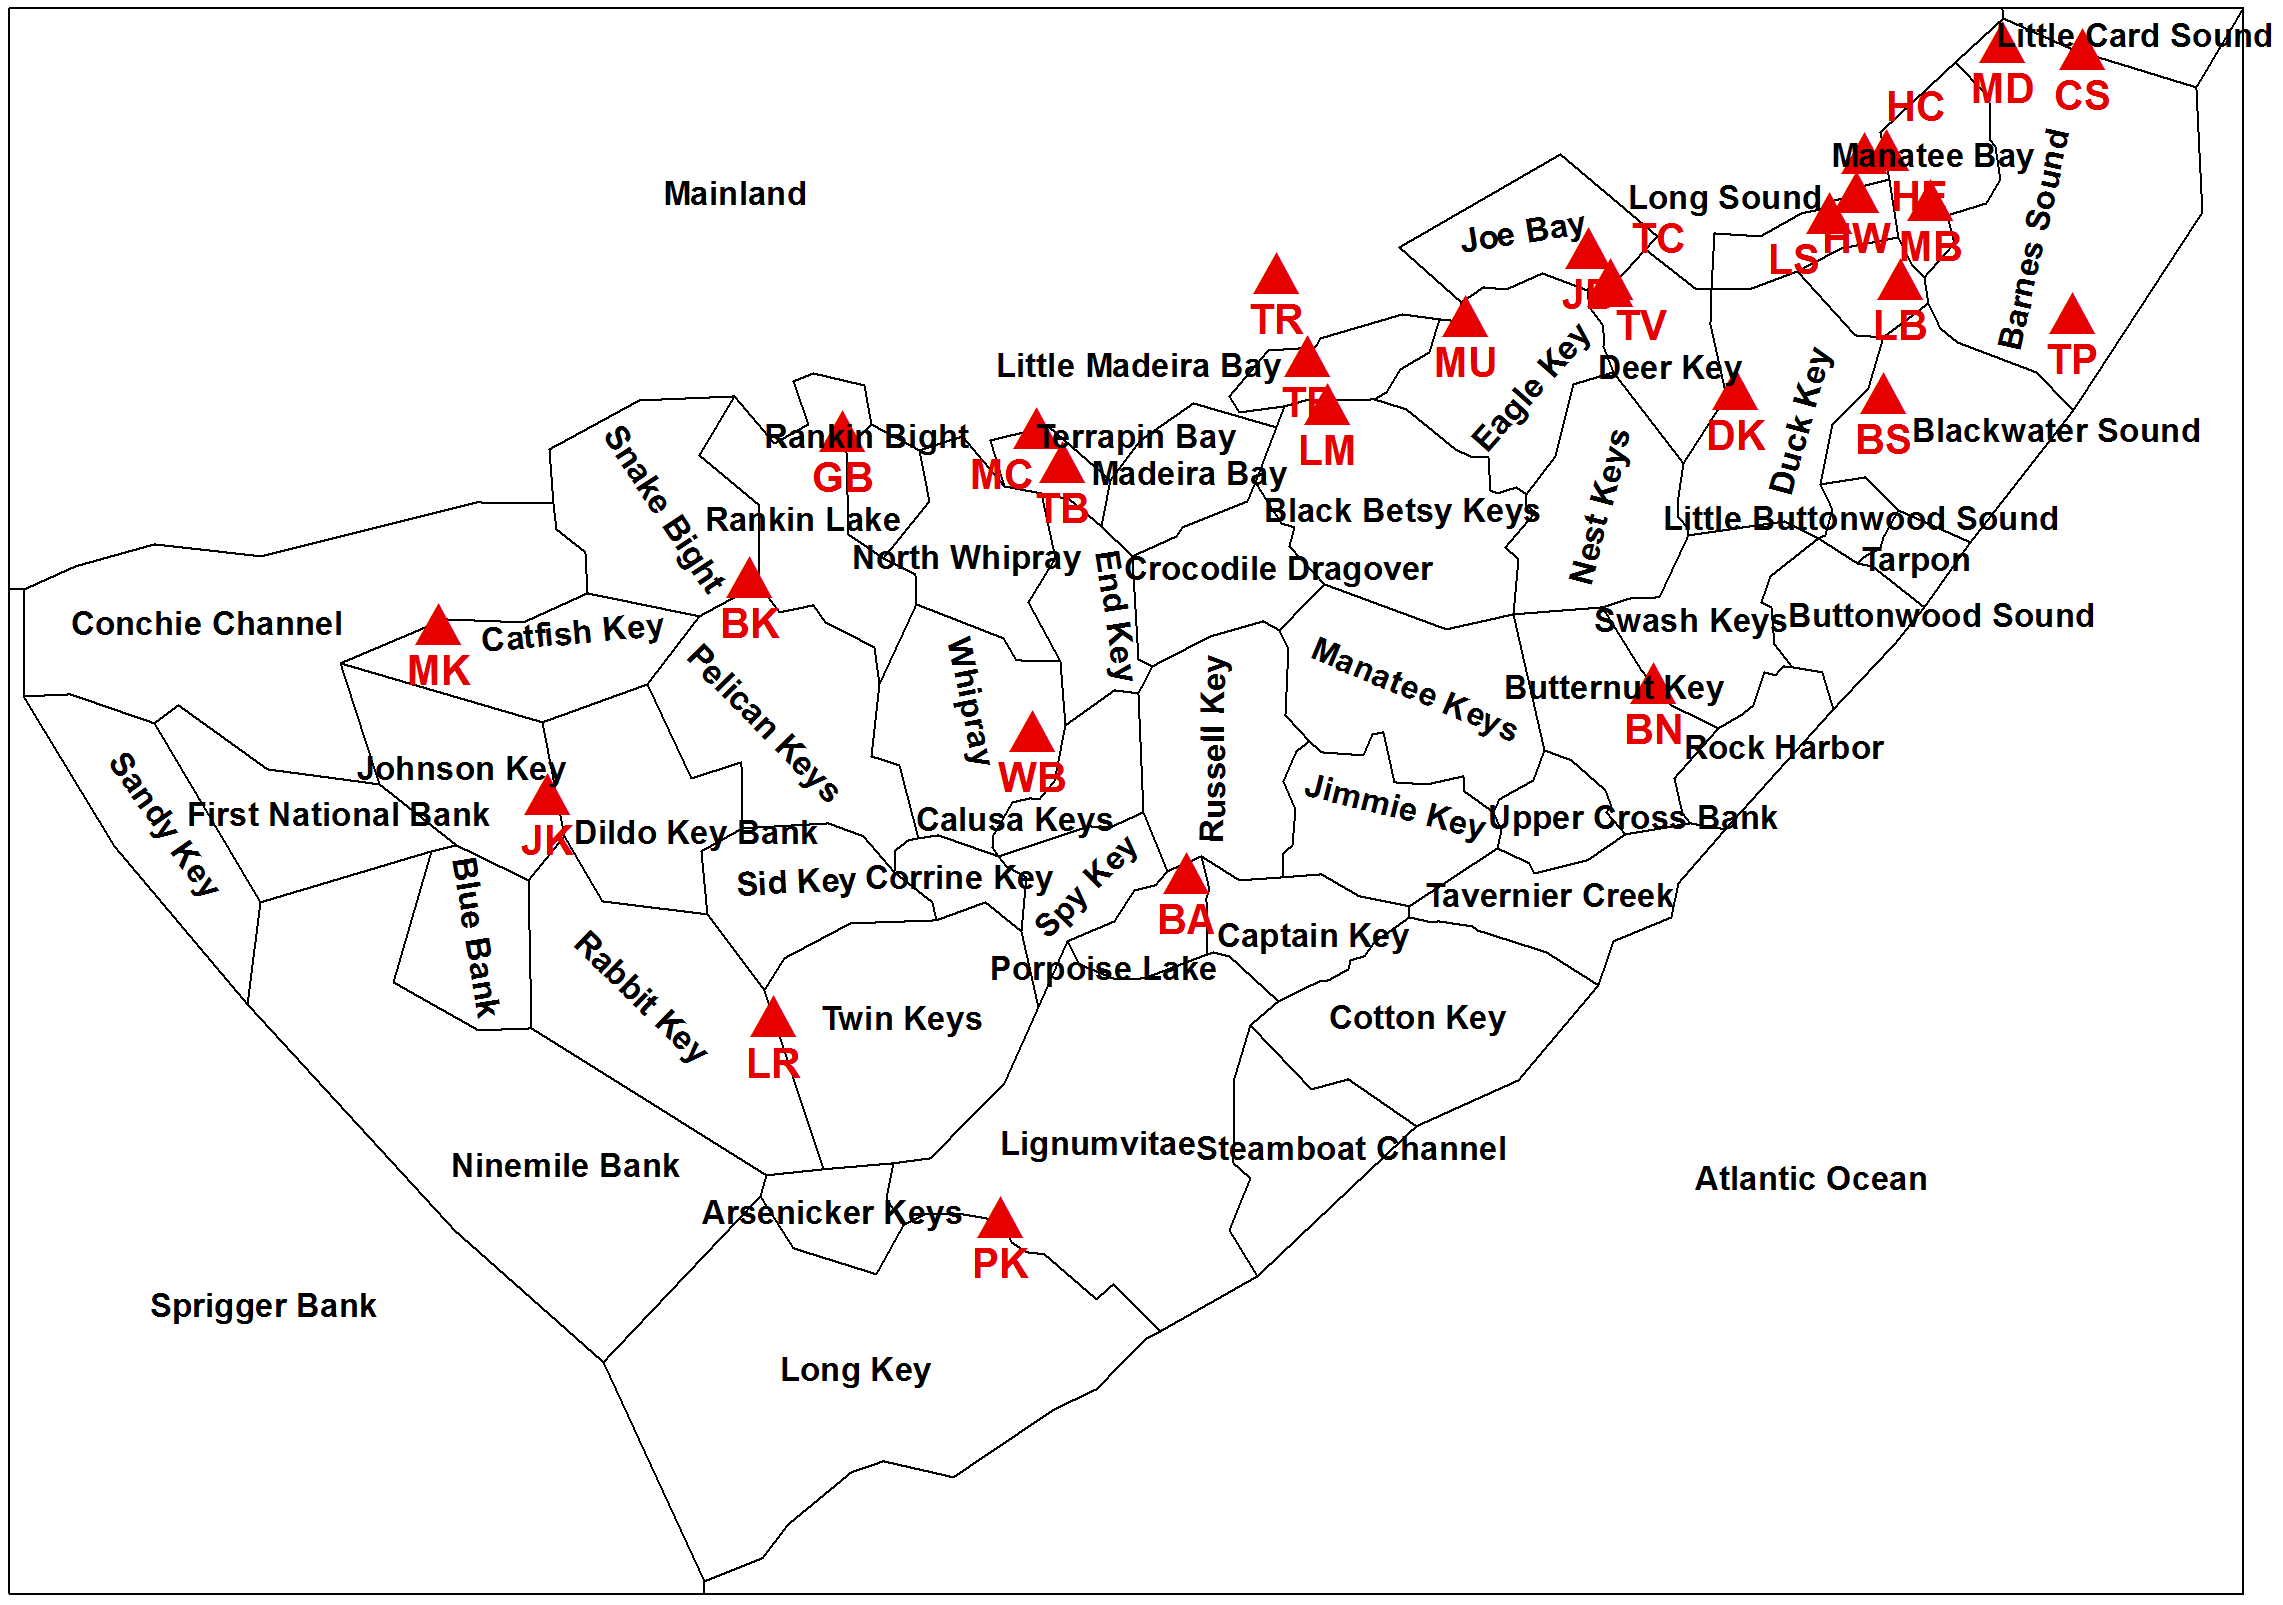
\includegraphics[ width = 0.77\textwidth ]{graphics/BAM_Basins_Stations.png}
  }
  {
     \caption{ \newline \newline BAM domain with basins and hydrographic 
               stations (red). }
     \label{fig:BAM Domain}
  }
\end{figure}
%~~~~~~~~~~~~~~~~~~~~~~~~~~~~~~~~~~~~~~~~~


%----------------------------------------------------------------
%----------------------------------------------------------------
\clearpage 
\section{Physical Representation}
\label{sec:Physical Representation}
%----------------------------------------------------------------
%----------------------------------------------------------------
The physical basis of BAM is exceedingly simple.  Mass-transport over shoals is governed by the transport velocity $v$ integrated over the shoal depth and length
\begin{equation}
   v = \sqrt{2 g \, \frac{h_u - h_d}{1 + f}}
   \label{equ:Shoal Velocity}
\end{equation}
where $h_u$ and $h_d$ are the upstream and downstream basin water levels, and $f$ a friction factor
\begin{equation}
  f = 2 g \, n^2 \, w \, \rho^{-4/3}
  \label{equ:Shoal Friction}
\end{equation}
where $n$ is the Mannings coefficient, $w$ the shoal width, $\rho$ the shoal hydraulic radius and $g$ the vertical acceleration.  The module \texttt{hydro.py} contains all hydraulic computations. 

The mass flux of dissolved substances over each shoal $M$ ($\mathrm{g}$) is calculated as the product of the concentration of the substance in the water $C$ ($\mathrm{g \, m^{-3}}$) and the water mass flux $F$ ($\mathrm{m^{3} \, s^{-1}}$) on each shoal.  The mass fluxes $M$ are summed around the boundary of each basin, the net mass flux over the shoals is multiplied by the time step and, along with other inputs and outputs of mass during the time step, added to the mass in the basin at the beginning of the time step. The new mass is divided by the water volume to estimate the concentration at the end of the time step. 


%----------------------------------------------------------------
%----------------------------------------------------------------
\clearpage 
\section{Input}
\label{sec:Input}
%----------------------------------------------------------------
%----------------------------------------------------------------
BAM inputs are derived from a variety of sources, and with the exception of the Sea Level and Tide data are daily values specific to each basin in the domain.  Sea Level is a monthly value applied to all Gulf and Ocean boundary basins, while Tides are interpolated to the model timestep from hourly tide data.  The data files and their periods of record are listed in table \ref{table:Input Data Files and Periods}. 

%=========================================
\begin{table}[H]
\caption{
Input data files, period of record and command line option. Note that Salinity and Stage inputs are used for model output comparison, not as explicit model inputs.  However, salinity timeseries can be imposed on basins with the \texttt{--gaugeSalinity} command line option. 
} 
\centering
\begin{tabular}{ l l l l c }
\hline
Variable  & File & Start & End & Option \\
\hline
Rain      & DailyRainFilled\_cm\_1999-9-1\_2015-12-8.csv
          & 1999-09-01 & 2015-12-08 & \texttt{-br} \\
ET        & PET\_1999-9-1\_2015-12-8.csv
          & 1999-09-01 & 2015-12-08 & \texttt{-et} \\
Tide      & HourlyTide1990\_2020.tar.gz
          & 1990-01-01 & 2021-01-01 & \texttt{-bt} \\
Sea Level & MSL\_Anomaly.csv
          & 1999-08-15 & 2015-12-15 & \texttt{-msl} \\
Runoff    & EDEN\_Stage\_OffsetMSL.csv
          & 1999-09-01 & 2015-12-31 & \texttt{-bR} \\
Flow      & S197\_Flow\_1999-9-1\_2016-3-31.csv
          & 1999-09-01 & 2016-03-31 & \texttt{-bc} \\
Salinity  & DailySalinityFilled\_1999-9-1\_2015-12-8.csv
          & 1999-09-01 & 2015-12-08 & \texttt{-sf} \\
Stage     & DailyStage\_1999-9-1\_2016-3-1.csv 
          & 1999-09-01 & 2016-03-01 & \texttt{-bs} \\
\hline
\end{tabular}
\label{table:Input Data Files and Periods}
\end{table}
%=========================================

The input files listed in table \ref{table:Input Data Files and Periods} are created from the raw data with a series of R or Python scripts found in the \texttt{etc/} directory.  These files include\\[-0.5in]
\small
\begin{enumerate}
  \itemsep-8pt
  \item \texttt{CreateRainData.R}
  \item \texttt{CreateET.R}
  \item \texttt{CreateTideData.py}
  \item \texttt{CreateRegion.2.3.tide.R}
  \item \texttt{EDEN\_Stage.R}
  \item \texttt{CreateSalinityData.R}
  \item \texttt{Boundary.Salinity.R}
  \item \texttt{CreateStageData.R}
\end{enumerate}
\large

%----------------------------------------------------------------
\subsection{Basins}
\label{sec:Input Basins}
%----------------------------------------------------------------

Basins and their associated observational data stations are listed in table \ref{table:Basins Stations}.  Basins numbered 5 - 58 are the 54 basins representing Florida Bay, basins 1 - 4 are not used. Basins 59 - 68 are boundary basins representing Gulf of Mexico and ocean boundaries, and basins 69 - 82 are boundary basins of the Everglades. Each of the boundary basins has a one-to-one mapping to a basin in the model domain as described in the appropriate section (Tides section \ref{sec:Tides}, or Runoff section \ref{sec:Input Data Runoff}). 

%=========================================
\begin{table}[H]
\caption{
BAM basin numbers, names and observational data/boundary stations. 
} 
\centering
\begin{tabular}{ l l l | l l l }
\hline
Basin &   Name                   & Gauge & Basin &   Name           & Gauge\\
\hline
5     &  Barnes Sound            & MD    & 44 & Dildo Key Bank      & None\\
6     &  Manatee Bay             & MB    & 45 & Tavernier Creek     & None\\
7     &  Long Sound              & LS    & 46 & Butternut Key       & BN\\
8     &  Little Blackwater Sound & LB    & 47 & Duck Key            & DK\\
9     &  Blackwater Sound        & BS    & 48 & Manatee Keys        & None\\
10    &  Tarpon                  & None  & 49 & Swash Keys          & BN\\
11    &  Little Buttonwood Sound & None  & 50 & Deer Key            & TC\\
12    &  Nest Keys               & None  & 51 & Eagle Key           & None\\
13    &  Joe Bay                 & TC    & 52 & Steamboat Channel   & None\\
14    &  Little Madeira Bay      & LM    & 53 & Arsenicker Keys     & None\\
15    &  Black Betsy Keys        & LM    & 54 & Sid Key             & None\\
16    &  Upper Cross Bank        & None  & 55 & Pelican Keys        & None\\
17    &  Rock Harbor             & None  & 56 & Blue Bank           & None\\
18    &  Buttonwood Sound        & None  & 57 & First National Bank & None\\
19    &  Jimmie Key              & None  & 58 & Sandy Key           & None\\
20    &  Cotton Key              & None  & 59 & Gulf Tide 1         & Gulf\_1\\
21    &  Captain Key             & None  & 60 & Gulf Tide 2         & Gulf\_1\\
22    &  Russell Key             & None  & 61 & Gulf Tide 3         & Gulf\_1\\
23    &  Crocodile Dragover      & None  & 62 & Gulf Tide 4         & Gulf\_1\\
24    &  Madeira Bay             & None  & 63 & Ocean Tide 5        & Ocean\_1\\
25    &  Terrapin Bay            & None  & 64 & Ocean Tide 6        & Ocean\_1\\
26    &  End Key                 & None  & 65 & Ocean Tide 7        & Ocean\_1\\
27    &  Calusa Keys             & None  & 66 & Ocean Tide 8        & Ocean\_1\\
28    &  Spy Key                 & None  & 67 & Ocean Tide 9        & Ocean\_1\\
29    &  Porpoise Lake           & BA    & 68 & Card Sound Tide 10  & Ocean\_1\\
30    &  Lignumvitae             & PK    & 69 & EVER to Snake Bight     & S15\\
31    &  Long Key                & None  & 70 & EVER to Rankin Lake     & S16\\
32    &  Twin Keys               & LR    & 71 & EVER to Rankin Bight    & S16\\
33    &  Corrine Key             & None  & 72 & EVER to North Whipray   & S16\\
34    &  Whipray                 & WB    & 73 & EVER to Terrapin Bay    & S17\\
35    &  North Whipray           & None  & 74 & EVER to Madeira Bay     & S17\\
36    &  Rankin Bight            & None  & 75 & EVER to Little Madeira Bay & S18\\
37    & Rankin Lake              & GB    & 76 & EVER to Eagle Key       & S19\\
38    & Rabbit Key               & LR    & 77 & EVER to Joe Bay         & S20\\
39    & Johnson Key              & JK    & 78 & EVER to Deer Key        & S21\\
40    & Catfish Key              & MK    & 79 & EVER to Long Sound      & S22\\
41    & Snake Bight              & BK    & 80 & EVER to Manatee Bay     & S22\\
42    & Conchie Channel          & None  & 81 & EVER to Conchie Channel & S15\\
43    & Ninemile Bank            & None  & 82 & EVER to Barnes Sound    & S22\\
\hline
\end{tabular}
\label{table:Basins Stations}
\end{table}
%=========================================

The basin parameter file defines mappings between basins and observational gauges, as well as boundary basins and their input timeseries. This file is specified with the \texttt{-bp [--basinParameter]} option (default: \texttt{Basin\_Parameters.csv}).

The basin shapefile is specified with the \texttt{-bn [--basins]} option (default: \texttt{data/GIS/FLBayBasins}).

Bathymetry is described in the \texttt{-bd [--basinDepth]} file (default: \texttt{Basin\_Area\_Depth.csv}).  

Initial values of basin variables are set from the \texttt{-bi [--basinInit]} file (default: \texttt{Basin\_Initial\_Values.csv}).  However, for basins where observations are available the \texttt{-si [--salinityInit]} option (default: \texttt{yes}) will override the initial salinity values set from \texttt{basinInit} with observed data.

%----------------------------------------------------------------
\subsection{Shoals}
\label{sec:Input Shoals}
%----------------------------------------------------------------
Shoals are links between basins, and the objects where mass transport is quantified.  The structure of the model is dictated by the basin-shoal linkage in the \texttt{-sp [--shoalParameters]} file (default: \texttt{Shoal\_Parameters.csv}).  

The shoals shapefile is specified with the \texttt{-s [--shoals]} option (default: \texttt{data/GIS/FathomLines}). 

Shoal bathymetry and width is defined in the \texttt{-sl [--shoalLength]} file (default: \texttt{Shoal\_Length\_Depth.csv}). Mannings friction coefficients are also specified in the \texttt{shoalLength} file.

The user can override the Mannings coefficients specified in \texttt{shoalParameters} with the \texttt{-sm [--shoalManning]} option (default: \texttt{None}).  Use of this option will set the Mannings coefficient for all shoals in the model to the single specified value. 

%----------------------------------------------------------------
\subsection{Rain}
\label{sec:Input Data Rain}
%----------------------------------------------------------------
Rain input is based on observational data from the Marine Monitoring stations show in figure \ref{fig:BAM Domain}.  Since data coverage is not continuous, a resampling scheme is used to estimate surrogate values for missing data at each station.  Data from each station is first partitioned into rain observations for each day of the year over the period of record.  Data for a missing day is reconstructed by randomly sampling from the partitioned data for that day over all years.  This preserves the seasonal distribution of rainfall while allowing for natural variability.

Observed and reconstructed rain at the stations in eastern Florida Bay is shown in figure \ref{fig:East Florida Bay rain}, and for the western basins in figure \ref{fig:West Florida Bay rain}.

%~~~~~~~~~~~~~~~~~~~~~~~~~~~~~~~~~~~~~~~~~
\begin{figure}[H]
\begin{center}
  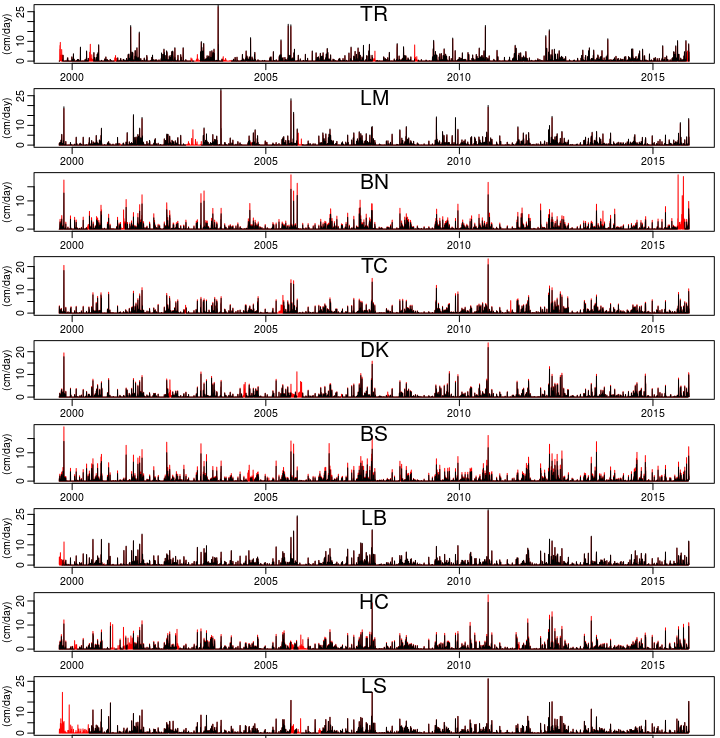
\includegraphics[ width = 0.95\textwidth ]{graphics/EastFLBayRainFilled.png}
  \caption{ East Florida Bay observed rain (black) and reconstructed rain (red). }
  \label{fig:East Florida Bay rain}
\end{center}
\end{figure}
%~~~~~~~~~~~~~~~~~~~~~~~~~~~~~~~~~~~~~~~~~

%~~~~~~~~~~~~~~~~~~~~~~~~~~~~~~~~~~~~~~~~~
\begin{figure}[H]
\begin{center}
  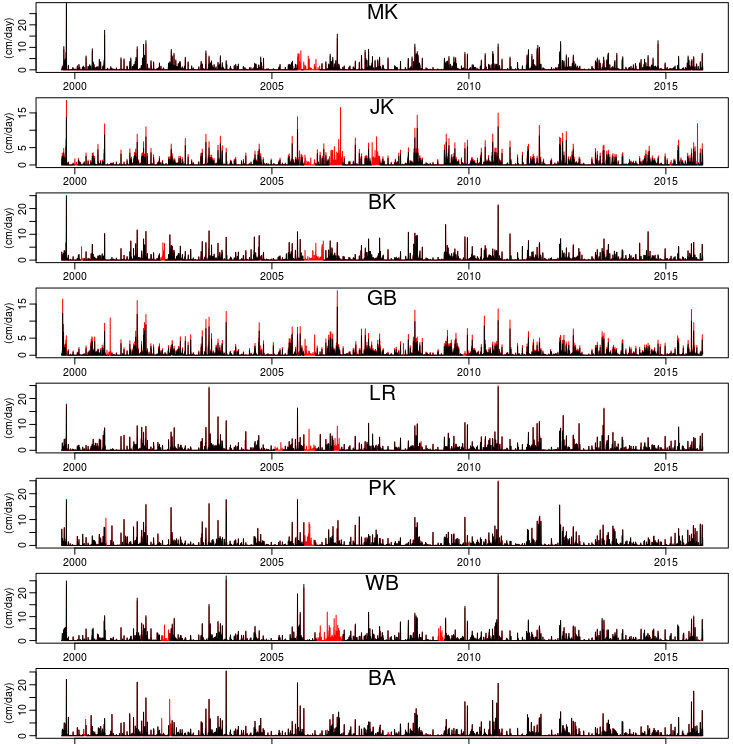
\includegraphics[ width = 0.95\textwidth ]{graphics/WestFLBayRainFilled.png}
  \caption{ West Florida Bay observed rain (black) and reconstructed rain (red). }
  \label{fig:West Florida Bay rain}
\end{center}
\end{figure}
%~~~~~~~~~~~~~~~~~~~~~~~~~~~~~~~~~~~~~~~~~
\clearpage

Estimation of total rain over basins tens to hundreds of square kilometers in area is notoriously challenging based on sparse, point measurements.  To afford the user control over the selection and effective areal input of rain, a mapping of basin to rain gauge stations is specified in the basin parameters (\texttt{-bp, [--basinParameter]}) file.  An excerpt of the basin parameter file is shown here:
\small
\begin{verbatim}
Basin,       Name,            Rain Gauge,   Rain Scale, Gauge
8,   Little Blackwater Sound, [ LS LB BS ], [ 3 2 3 ],  LB
9,   Blackwater Sound,        [ DK BS LB ], [ 2 3 2 ],  BS
10,  Tarpon,                  [ BS BN DK ], [ 2 2 1 ],  None
11,  Little Buttonwood Sound, [ BS BN DK ], [ 1 2 2 ],  None
\end{verbatim}
\large

The \texttt{Rain Gauge} column defines a list of rain gauges aggregated to produce the input rainfall for a basin.  The \texttt{Rain Scale} is a corresponding list of scale factors applied to each rain gauge data value in the gauge list.  This allows complete control over the basin rain input, and has been found to give good spatial smoothing to compensate for the fact that point measurements of rain are often insufficient to represent total rain volumes over a large areal extents. 

The rain input file is specified with the \texttt{-br [--basinRain]} option, and has a default value of \texttt{DailyRainFilled\_cm\_1999-9-1\_2015-12-8.csv}.  Rain inputs can be disabled by specifying the \texttt{-nr [--noRain]} option, which has a default value of \texttt{False}. 

%----------------------------------------------------------------
\subsection{ET}
\label{sec:Input Data ET}
%----------------------------------------------------------------
Evapotranspiration (ET) data are obtained from the South Florida Water Management District (SFWMD) measuring stations at Joe Bay in the C-111 basin (JBTS\_C111), structure S331 in the L31N basin (S331W\_L31NS), and a three station average in water conservation area 3A of the WCA3A basin (3AS3WX\_WCA3).  Note that these basins are not in Florida Bay.  

A single timeseries is created by taking the maximum value of the three data sets for any given day which covers most data gaps.  The remaining gaps are reconstructed with a resampling scheme where the data are partitioned into samples for each day of the year over the period of record and missing data randomly drawn from the samples for a specific yearday. Figure \ref{fig:BAM ET} plots the resultant ET data which is applied to all basins in the model. 

%~~~~~~~~~~~~~~~~~~~~~~~~~~~~~~~~~~~~~~~~~
\begin{figure}[H]
  \floatbox[{ \capbeside\thisfloatsetup{ capbesideposition = {right, center},
                                         capbesidewidth = 4cm } }]
  {figure}[\FBwidth]
  {
     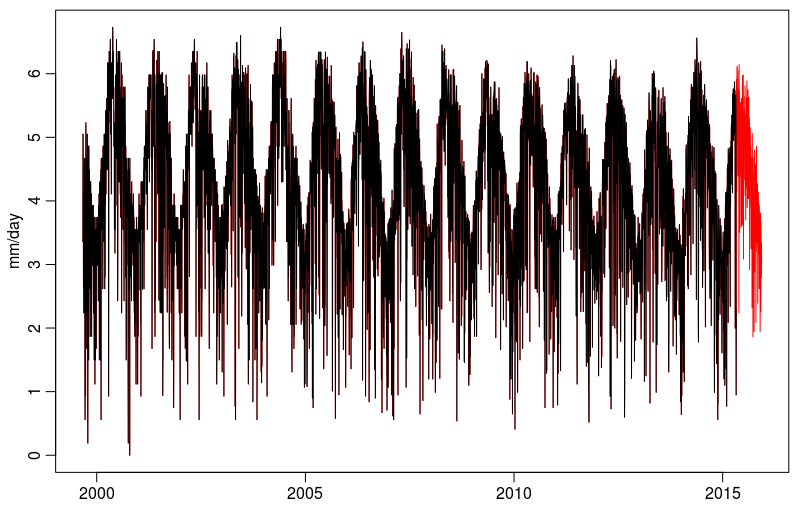
\includegraphics[ width = 0.75\textwidth ]{graphics/BAM_ET.png}
  }
  {
     \caption{ \newline \newline SFWMD observed ET (black) and 
               reconstructed ET (red). }
     \label{fig:BAM ET}
  }
\end{figure}
%~~~~~~~~~~~~~~~~~~~~~~~~~~~~~~~~~~~~~~~~~

To provide user control over the magnitude of ET, the \texttt{-es [--ET scale]} command line option applies a scale factor to the data shown in figure \ref{fig:BAM ET}. 

The ET input file is specified with the \texttt{-et [--ET]} option, and has a default value of \texttt{PET\_1999-9-1\_2015-12-8.csv}.  ET inputs can be disabled by specifying the \texttt{-ne [--noET]} option, which has a default value of \texttt{False}. 

%----------------------------------------------------------------
\subsection{Everglades Runoff}
\label{sec:Input Data Runoff}
%----------------------------------------------------------------
The BAM convention for basin runoff is that positive runoff corresponds to flow leaving the basin, while negative runoff quantifies flow entering the basin.  

A hydraulic head relationship exists between water levels in the southern Everglades and freshwater runoff into the coastal basins as expressed in strong negative correlations between Everglades water level and coastal basin salinity \citep{Tabb1967, Kelble2007}.  BAM uses this relationship to estimate integrated Everglades runoff (streamflow, sheetflow and groundwater) into the coastal basins by the same shoal hydraulics as all other interbasin flows.  Shoal parameters are calibrated to match runoff values determined by FATHOM \citep{Cosby2010} in section \ref{sec:Runoff Calibration}.

Upstream basins representing the Everglades have water levels determined by values extracted from the Everglades Depth Estimation Network (EDEN) at eight stations shown in figure \ref{fig:EDEN Stations} and table \ref{table:EDEN Stations}.  These water levels are converted from NAVD to water level anomalies with respect to Florida Bay mean sea level over the period 2008 - 2015. 

%~~~~~~~~~~~~~~~~~~~~~~~~~~~~~~~~~~~~~~~~~
\begin{figure}[H]
  \floatbox[{ \capbeside\thisfloatsetup{ capbesideposition = {right, center},
                                         capbesidewidth = 4cm } }]
  {figure}[\FBwidth]
  {
     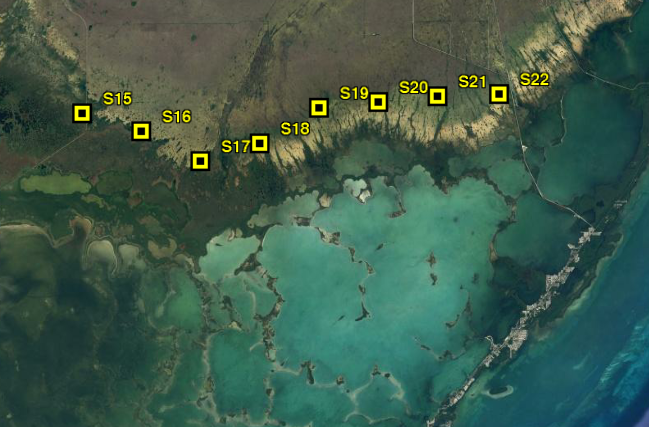
\includegraphics[width=0.75\textwidth]{graphics/EDEN_Stations.png}
  }
  {
     \caption{ \newline \newline Eight stations in the southern Everglades 
               where EDEN stage is extracted to provide hydraulic forcings 
               for runoff into the coastal basins. }
     \label{fig:EDEN Stations}
  }
\end{figure}
%~~~~~~~~~~~~~~~~~~~~~~~~~~~~~~~~~~~~~~~~~

%=========================================
\begin{table}[H]
  \floatbox[{ \capbeside\thisfloatsetup{ capbesideposition = {right, center},
                                         capbesidewidth = 4cm } }]
  {table}[\FBwidth]
  {
     \caption{ Coordinates of EDEN stations providing Everglades stage 
               to drive runoff. }
     \label{table:EDEN Stations}
  }
  {
    \centering
    \begin{tabular}{ c c c c c c }
      \hline
      Station & UTM North & UTM East & Zone & Longitude  & Latitude\\
      \hline
      S15     & 2794000   & 520000   & 17   & -80.801379 & 25.262235\\
      S16     & 2792500   & 525000   & 17   & -80.751752 & 25.248614\\
      S17     & 2790000   & 530000   & 17   & -80.702158 & 25.225945\\
      S18     & 2791500   & 535000   & 17   & -80.652480 & 25.239383\\
      S19     & 2794500   & 540000   & 17   & -80.602747 & 25.266350\\
      S20     & 2795000   & 545000   & 17   & -80.553075 & 25.270723\\
      S21     & 2795500   & 550000   & 17   & -80.503400 & 25.275079\\
      S22     & 2795700   & 555200   & 17   & -80.451747 & 25.276703\\
      \hline
    \end{tabular} 
  }
\end{table}
%=========================================

Water levels at the EDEN stations are shown in figure \ref{fig:EDEN Stage} exhibiting the expected seasonal uniformity, as well as deeper dry-season minima along the western bay.

%~~~~~~~~~~~~~~~~~~~~~~~~~~~~~~~~~~~~~~~~~
\begin{figure}[H]
  \floatbox[{ \capbeside\thisfloatsetup{ capbesideposition = {right, center},
                                         capbesidewidth = 4cm } }]
  {figure}[\FBwidth]
  { 
     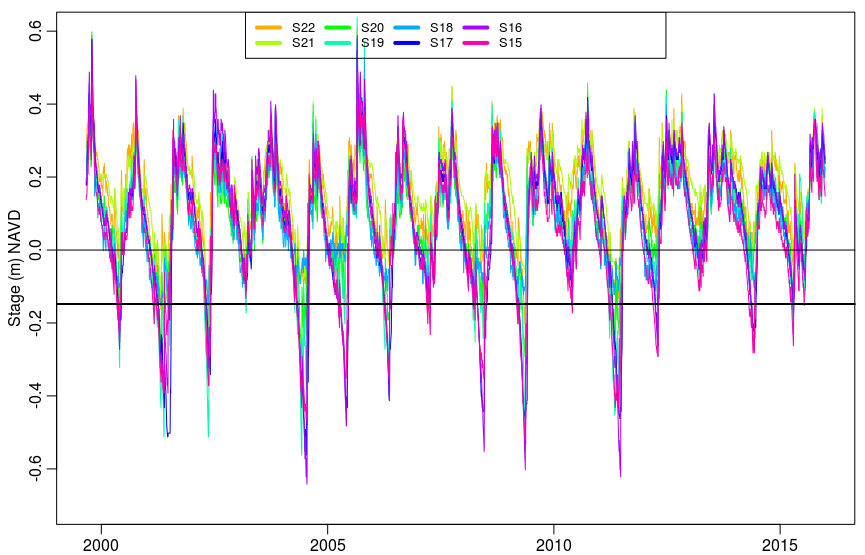
\includegraphics[ width = 0.75\textwidth ]{graphics/EDEN_BAM_Stage.png}
  }
  {
     \caption{ \newline \newline EDEN stage at eight stations in the 
               southern Everglades. Mean sea level (2008-2015) is shown 
               by the line at -14.8 cm. }
     \label{fig:EDEN Stage}
  }
\end{figure}
%~~~~~~~~~~~~~~~~~~~~~~~~~~~~~~~~~~~~~~~~~

The EDEN stage file used to drive runoff is specified with the \texttt{-bR [--basinStageRunoff]} option with a default value of \texttt{EDEN\_Stage\_OffsetMSL.csv}.  The mapping of EDEN stage values to coastal basins and the corresponding shoals is specified with the \texttt{-bS [--basinStageRunoffMap]} with a default of \texttt{Basin\_Runoff\_Boundary.csv}.  Runoff from the hydraulic stage relationship can be disabled with the \texttt{-nR [--noStageRunoff]} option which has a default of \texttt{False}.  An example of the EDEN stage to coastal basin runoff mapping file is shown below.

\small
\begin{verbatim}
Source_Basin, EDEN, Dest_Basin, Dest_Name,         Shoals
82,           S22,  5,          Barnes Sound,      [ 373 ]
80,           S22,  6,          Manatee Bay,       [ 333 334 ]
79,           S22,  7,          Long Sound,        [ 336 337 338 339 340 341 342 343 ]
77,           S20,  13,         Joe Bay,           [ 348 358 359 360 ]
75,           S18,  14,         Little Madeira Bay,[ 168 169 170 171 172 173 174 ]
74,           S17,  24,         Madeira Bay,       [ 149 150 151 ]
73,           S17,  25,         Terrapin Bay,      [ 142 143 144 ]
72,           S16,  35,         North Whipray,     [ 126 127 ]
71,           S16,  36,         Rankin Bight,      [ 135 ]
70,           S16,  37,         Rankin Lake,       [ 136 137 138 139 140 141 ]
69,           S15,  41,         Snake Bight,       [ 24 25 26 ]
78,           S21,  50,         Deer Key,          [ 346 347 ]
76,           S19,  51,         Eagle Key,         [ 356 357 ]
81,           S15,  42,         Conchie Channel,   [ 6 7 8 9 10 ]
\end{verbatim}
\large

%----------------------------------------------------------------
\subsection{Tides}
\label{sec:Tides}
%----------------------------------------------------------------
Tidal variations are a primary driver of hydraulic fluxes throughout Florida Bay.  In order to accurately estimate basin water levels and thereby the associated mass transports between basins BAM uses local, hourly tidal estimates as the foundation for tidal boundary conditions.  These estimates are computed from NOAA subordinate station harmonic constituents at the stations listed in table \ref{table:Tide Stations}.  The resultant tidal data contain all astronomical forcings, but do not include variations of secular sea level rise or annual and interannual cycles from ocean currents and atmospheric teleconnections.  Those are accounted in section \ref{sec:Sea Level}. 

%=========================================
\begin{table}[H]
  \floatbox[{ \capbeside\thisfloatsetup{ capbesideposition = {right, center},
                                         capbesidewidth = 4cm } }]
  {table}[\FBwidth]
  {
     \caption{ NOAA subordinate tide stations where tides are calculated 
               along the gulf and ocean boundaries. }
     \label{table:Tide Stations}
  }
  {
    \centering
    \begin{tabular}{ l l }
      \hline
      Name & Station ID\\
      \hline
      Cape Sable, East Cape, Florida                        & TEC4165\\
      Long Key, western end, Florida                        & 8723899\\
      Lignumvitae Key, NE side, Florida Bay, Florida        & 8723824\\
      Snake Creek, Hwy. 1 bridge, Windley Key, Florida      & 8723787\\
      Tavernier Creek, Hwy. 1 bridge, Hawk Channel, Florida & 8723748\\
      Garden Cove, Key Largo, Florida                       & 8723622\\
      Little Card Sound bridge, Florida                     & 8723534\\
      \hline
    \end{tabular}
  }
\end{table}
%=========================================

Timeseries for the stations in table \ref{table:Tide Stations} are generated by the \texttt{CreateTideData.py} and \newline \texttt{CreateRegion.2.3.tide.R} programs. 

Basins numbered 59 - 68 are tidal boundary basins, each one connected to a Florida Bay basin as specified in the \texttt{shoalParameters} file and shown in table \ref{table:Tide Basin Shoals}. 

%=========================================
\begin{table}[H]
  \floatbox[{ \capbeside\thisfloatsetup{ capbesideposition = {right, center},
                                         capbesidewidth = 4cm } }]
  {table}[\FBwidth]
  {
     \caption{ Tide boundary basin and shoal mapping. Boundary basin names 
               corresponds to the basin Gauge listed in 
               table \ref{table:Basins Stations}. }
     \label{table:Tide Basin Shoals}
  }
  {
    \centering
    \begin{tabular}{ l c l c l }
      \hline
      Name            & Basin & Name    & Basin & Shoals\\
      \hline
      Conchie Channel   &  42 & Gulf\_1   & 59 & 23\\
      Sandy Key         &  58 & Gulf\_2   & 60 & 22 370\\
      Ninemile Bank     &  43 & Gulf\_3   & 61 & 45 371\\
      Long Key          &  31 & Gulf\_4   & 62 & 70\\
      Long Key          &  31 & Ocean\_5  & 63 & 64 65 66 67 68\\
      Long Key          &  31 & Ocean\_6  & 64 & 61 62 63 239 237\\
      Lignumvitae       &  30 & Ocean\_6  & 64 & 237\\
      Steamboat Channel &  52 & Ocean\_7  & 65 & 240\\
      Cotton Key        &  20 & Ocean\_7  & 65 & 241 242\\
      Tavanier Creek    &  45 & Ocean\_8  & 66 & 271 272 273 274\\
      Rock Harbor       &  17 & Ocean\_8  & 66 & 288\\
      Buttonwood Sound  &  18 & Ocean\_9  & 67 & 289 290\\
      Tarpon            &  10 & Ocean\_9  & 67 & 309\\
      Blackwater Sound  &  9  & Ocean\_9  & 67 & 310\\
      Barnes Sound      &  5  & Ocean\_9  & 67 & 365 366\\
      Barnes Sound      &  5  & Ocean\_10 & 68 & 362 363\\
      \hline
    \end{tabular}
  }
\end{table}
%=============================

There are no NOAA stations along western Florida Bay between Cape Sable and Long Key.  Examination of tidal response at these two stations shows that tides at Long Key are delayed by 6 - 8 hours and attenuated by a factor of 2.7 - 3 in relation to Cape Sable.  To estimate tidal responses between these two points it is assumed that the upper region tides are 2/3 the amplitude and 3 hours delayed from Cape Sable, while the lower region is 4/3 the amplitude and 3 hours prior to Long Key.  These amplitude and phase modulations are performed in \texttt{CreateRegion.2.3.tide.R} producing the tidal forcings for the \texttt{Gulf\_2} and \texttt{Gulf\_3} boundaries.  A graphical comparison shows that these assumptions give a reasonable transitional tidal response between Cape Sable and Long Key.

The mapping between boundary basin tidal heights and tidal timeseries is specified in the \texttt{-bt --basinTide} file (default: \texttt{Basin\_Tide\_Boundary\_2010\_2015.csv}).  If the \texttt{-nt [--noTide]} option (default: \texttt{False}) is activated, no tidal data are applied at the boundaries. 

BAM interpolates the hourly tidal timeseries to the model timestep at runtime based on cubic spline fits to the hourly data.  The cubic splines are generated during model initialization and this process can be time consuming.  Two approaches are used to minimize this process.  First, the spline generations are parallel processed by up to 4 processors (if available).  Second, subsets of hourly tidal data can be specified in the \texttt{basinTide} file that correspond to the model simulation period, say 2010-1-1 to 2015-12-31 instead of the entire model period of record.

An example of tidal boundary data and the corresponding basin response is depicted in figure \ref{fig:Tide example}.

%~~~~~~~~~~~~~~~~~~~~~~~~~~~~~~~~~~~~~~~~~
\begin{figure}[H]
  \floatbox[{ \capbeside\thisfloatsetup{ capbesideposition = {right, center},
                                         capbesidewidth = 4cm } }]
  {figure}[\FBwidth]
  {
    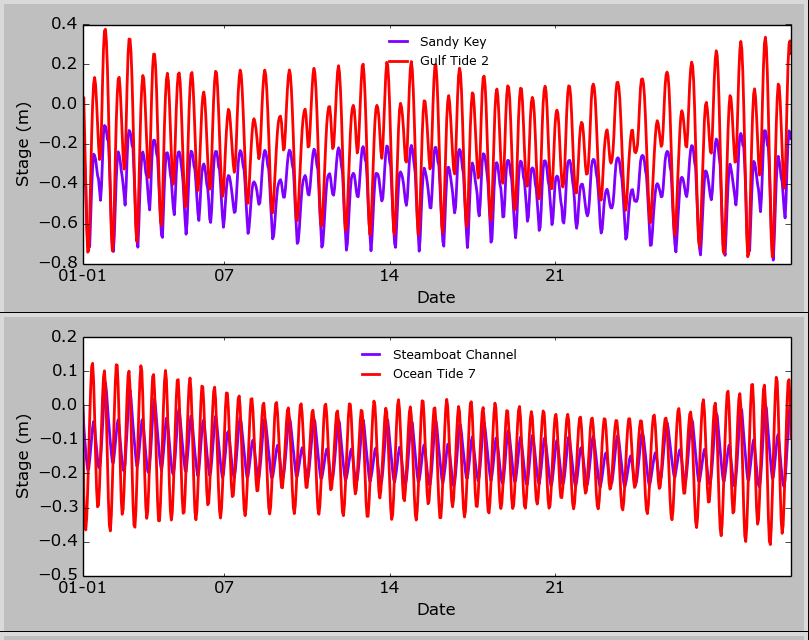
\includegraphics[ width = 0.75\textwidth ]{graphics/BAM_Tide.png}
  }
  {
     \caption{ \newline \newline Tidal boundary conditions (red) and 
               corresponding basin water levels (blue) for the period 
               2010-1-1 through 2010-1-31. }
     \label{fig:Tide example}
  }
\end{figure}
%~~~~~~~~~~~~~~~~~~~~~~~~~~~~~~~~~~~~~~~~~


%----------------------------------------------------------------
\subsection{Sea Level}
\label{sec:Sea Level}
%----------------------------------------------------------------
Tidal data are local and derived from astronomically-forced harmonic constituents fit to water level observations. As such, they do not include sea level response to regional ocean currents, atmospheric teleconnections or secular sea level rise.  To address this the \texttt{-msl [--seasonalMSL]} file (default: \texttt{MSL\_Anomaly.csv}) specifies a regional mean sea level anomaly timeseries superimposed on the tidal boundary data.  Regional sea levels are not applied if the \texttt{-nm [--noMeanSeaLevel]} option (default: \texttt{False}) is activated. 

The default regional sea levels in \texttt{MSL\_Anomaly.csv} are determined from monthly mean sea level data at the three long-term, primary NOAA tide stations  listed in table \ref{table:Sea Level Stations}.  Monthly mean sea levels published by NOAA have the annual seasonal cycle removed, and are with respect to the current (1983 - 2001) National Tidal Datum Epoch (NTDE) determination of mean sea level at each station.

%=========================================
\begin{table}[H]
  \floatbox[{ \capbeside\thisfloatsetup{ capbesideposition = {right, center},
                                         capbesidewidth = 4cm } }]
  {table}[\FBwidth]
  {
     \caption{ Long-term, primary NOAA tide gauges.  MSL is the 
               NTDE mean sea level datum elevation, and NAVD 
               the North American Vertical Datum elevation. }
     \label{table:Sea Level Stations}
  }
  {
    \centering
    \begin{tabular}{ l c c c c }
      \hline
      Station     & CO-OPS ID & Verified Data & NAVD (m) & MSL (m)\\
      \hline
      Virginia Key  & 8723214 & 1994 - 2016   & 3.698    & 3.431\\
      Vaca Key      & 8723970 & 1973 - 2016   & 1.182    & 0.931\\
      Key West      & 8724580 & 1954 - 2016   & 1.928    & 1.662\\
      \hline
    \end{tabular}
  }
\end{table}
%=========================================

To represent total mean sea level the annual seasonal cycle at each station is added to the published monthly sea levels and converted to the NAVD datum.  The three stations are then averaged to estimate a regional mean sea level timeseries on a common datum (RMS deviation of 1.7 cm). 

Finally, the mean sea level is converted from the NAVD datum to mean sea level in Florida Bay over the 2008-2015 period.  Mean sea level in Florida Bay is determined from an average of daily mean data smoothed with a 30-day moving average at stations LM, PK and MK.  This is necessary since BAM operates on water level anomalies rather than a geodetic reference.  The resultant sea level signal is shown in figure \ref{fig:MSL}.

%~~~~~~~~~~~~~~~~~~~~~~~~~~~~~~~~~~~~~~~~~
\begin{figure}[H]
  \floatbox[{ \capbeside\thisfloatsetup{ capbesideposition = {right, center},
                                         capbesidewidth = 4cm } }]
  {figure}[\FBwidth]
  {
    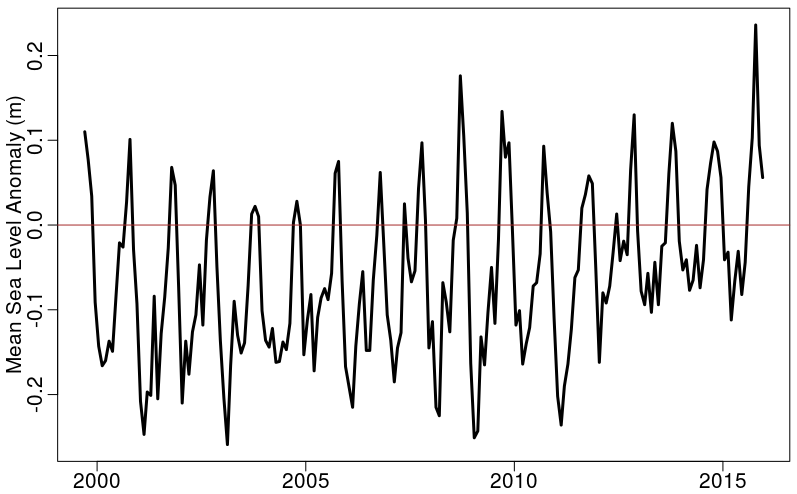
\includegraphics[ width = 0.75\textwidth ]{graphics/BAM_MSL.png}
  }
  {
     \caption{ \newline \newline Mean sea level anomaly with respect to 
               the 2008 - 2015 mean sea level in Florida Bay (-14.8 cm NAVD). }
     \label{fig:MSL}
  }
\end{figure}
%~~~~~~~~~~~~~~~~~~~~~~~~~~~~~~~~~~~~~~~~~

%----------------------------------------------------------------
\subsection{Basin Boundary Conditions}
\label{sec:Basin Boundary Conditions}
%----------------------------------------------------------------
Tidal and Everglades water levels constitute boundary conditions for the model imposing water levels on boundary basins which interact with basins of Florida Bay.  There are also two methods to impose stage or flow boundaries onto interior basins: fixed boundary conditions impose a constant stage or flow, dynamic boundary conditions impose values from a timeseries. 

{\bf Warning:} Stage boundary conditions are imposed at the start of each timestep. Currently, the basin water level is then updated according to changes in volume from mass transport. 

{\bf Warning:} Dynamic timeseries flow values are assumed to be in units of $\mathrm{ft^3\,s^{-1}}$.  Fixed timeseries flow values are specified in units of $\mathrm{m^3\,s^{-1}}$.

%-----------------------------------------
\subsubsection{Fixed Boundary Conditions}
\label{sec:Fixed Boundary Conditions}
%-----------------------------------------
Fixed boundary conditions are enabled with the \texttt{-fb [--fixedBoundaryConditions]} option (default: \texttt{False}).  When enabled, the forcings are specified in the \texttt{-bf [--basinFixedBCFile]} file (default: \texttt{Basin\_Fixed\_Boundary\_Condition.csv}).  An example of a \texttt{basinFixedBCFile} is shown below:

\begin{verbatim}
Basin, Name,      Type, Value
56,    Blue Bank, flow, 1000
\end{verbatim}

\texttt{Type} can have the value \texttt{stage} or \texttt{flow}. If \texttt{Type} is \texttt{flow} then at each model timestep the flow \texttt{Value} ($\mathrm{m^3\,s^{-1}}$) is multiplied by the model timestep interval converting the flow into a volume ($\mathrm{m^3}$).  This volume is added to the basin at the beginning of the timestep. 

If \texttt{Type} is \texttt{stage} then at each model timestep the basin water level is set to the stage \texttt{Value} at the beginning of the timestep.  This does not prevent the basin water level from being updated at the end of the timestep in response to mass transport. 

%-----------------------------------------
\subsubsection{Dynamic Boundary Conditions}
\label{sec:Dynamic Boundary Conditions}
%-----------------------------------------
Dynamic boundary conditions are enabled with the \texttt{-nb [--noDynamicBoundaryConditions]} option (default: \texttt{False}).  When enabled forcings are specified in the \texttt{-bc [--basinBCFile]} file (default: \texttt{Basin\_Boundary\_Condition.csv}). An example of a \texttt{basinBCFile} is shown below:

\begin{verbatim}
Basin, Name,        Type, File
6,     Manatee Bay, flow, data/Boundary/S197_Flow_1999-9-1_2016-3-31.csv
\end{verbatim}

\texttt{Type} can have the value \texttt{stage} or \texttt{flow}. If \texttt{Type} is \texttt{flow} then at each model timestep the flow value obtained from \texttt{File} is multiplied by 0.028317 to convert it from $\mathrm{ft^3\,s^{-1}}$ to $\mathrm{m^3\,s^{-1}}$.  The resulting value is multiplied by the model timestep interval to convert the flow to a volume ($\mathrm{m^3}$).  This volume is added to the basin at the beginning of the timestep. 

If \texttt{Type} is \texttt{stage} then at each model timestep the basin water level is set to the stage value obtained from the \texttt{File} at the beginning of the timestep.  This does not prevent the basin water level from being updated at the end of the timestep in response to mass transport. 

%----------------------------------------------------------------
\subsection{Salinity}
\label{sec:Salinity}
%----------------------------------------------------------------
Salinity is a primary output of the model and is not required as input to estimate basin salinities.  However, high-quality, long-period salinity available from marine monitoring stations affords several advantages to model operation and evaluation.  First, salinity in the gulf and ocean boundary basins has an important influence on salinities inside the bay.  Boundary salinity and runoff may be the most important exogenous variables for coastal basin salinity and good model results require accurate boundary salinities. 

Second, observed data can be used to initialize basin salinities with the \texttt{-si [--salinityInit]} option.  Third, basin salinities can be imposed from observed timeseries with the \texttt{-gs [--gaugeSalinity]} option.  If \texttt{-gs} is specified then all basins with salinity gauges listed in the \texttt{basinParameter -bp} file will have observed salinities imposed. Finally, the database of observed salinities allows the user to plot observed data against model data for evaluation and comparison purposes.

Salinity on the Gulf of Mexico boundary has significant variability in comparison to open ocean seawater.  Here, the Florida Shelf has a wide, flat and shallow bathymetry, with a generally weak, northerly countercurrent to the Loop current. This allows hypersaline conditions to develop during times of high evaporation and weak circulation.  The shelf also receives freshwater runoff from the Shark River and Everglades distributaries, and significant subtropical rain events can also contribute to hyposaline conditions.  Boundary salinity for this domain is computed from a 4-gauge average of daily mean salinity at the stations MK, JK, LR, PK, which has an overall standard deviation of 1.7 g/kg over the period September 1, 1999 to December 31, 2015 (N = 5943).

On the Atlantic side salinity is less variable than the Florida Shelf, but still ranges considerably in comparison to open ocean values.  The Lignumvitae basin (station PK) in southern Florida Bay is a predominantly marine environment with significant exchange with the Atlantic, and we use a six-month lowpass filter applied to the PK station salinity to represent Atlantic boundary salinities.

Observed salinities are specified in the \texttt{-sf [--salinityFile]} file \newline (default: \texttt{DailySalinityFilled\_1999-9-1\_2015-12-8.csv}). Boundary salinties are also included in this file with boundary data 'gauges' specified in the \texttt{basinParameter} file (for example: \texttt{Ocean\_1} and \texttt{Gulf\_1}).

Salinity observations are not continuous thereby a resampling scheme is used to estimate values of missing data at each station.  Data from each station is first partitioned into observations for each day of the year over the period of record.  Data for a missing day is reconstructed by randomly sampling from the partitioned data for that day over all years.

%----------------------------------------------------------------
\subsection{Basin Water Level}
\label{sec:Basin Water Level}
%----------------------------------------------------------------
Basins water levels are computed according to mass conservation of water across the shoals along with contributions from rainfall, ET, runoff and fixed boundary conditions.  Exceptions are the gulf and ocean boundary basins where water levels are imposed from tidal and sea level data.  

Since basin water levels provide the hydraulic potential for interbasin mass transfer, the availability of high-quality, long-period observational water levels is useful in the evaluation of model development and performance.  The graphical user interface provides graphical comparison of observed and modeled water levels. 

The water level data file is defined with the \texttt{-bs [--basinStage]} option \newline (default: \texttt{DailyStage\_1999-9-1\_2016-3-1.csv}).

%----------------------------------------------------------------
\subsection{Wind}
\label{sec:Wind}
%----------------------------------------------------------------
Wind is currently not used. 

%----------------------------------------------------------------
%----------------------------------------------------------------
\clearpage 
\section{Output}
\label{sec:Output}
%----------------------------------------------------------------
%----------------------------------------------------------------
Model output is exclusively in UTF-8 encoded comma-delimited variable (\texttt{.csv}) files.  Each basin in the model has a file created based on the basin name, for example \texttt{Long Sound.csv}. 

Basin output variables can be selected in the graphical user interface, default variables are \texttt{Salinity, Stage, Flow, Volume, Rain, Evaporation, Runoff}.

The output directory is defined by the \texttt{-bo [--basinOutput]} option with default: \texttt{home\_dir/BAM.out} where \texttt{home\_dir} is the value of the \texttt{HOME} environment variable if it is defined, otherwise the current working directory.

Messages generated during a model run are written to the \texttt{RunInfo.txt} file in the model output directory. 

Currently, no shoal output is created. 

%----------------------------------------------------------------
%----------------------------------------------------------------
\clearpage 
\section{Model Execution}
\label{sec:Model Execution}
%----------------------------------------------------------------
%----------------------------------------------------------------
BAM is a Python 3 application.  The model entry-point is the function \texttt{main()} in \texttt{bam.py} which is invoked by simply executing \texttt{bam.py} as a shell command.  To execute the model without the graphical user interface specify the \texttt{-ng [--noGUI]} option. 

%----------------------------------------------------------------
\subsection{Installation}
\label{sec:Installation}
%----------------------------------------------------------------
In addition to Python 3, several community modules such as SciPy are needed.  Installation notes can be found in the docstring of the Notes.py module and can be accessed from the Python console:
\small
\begin{verbatim}
>>> import Notes
>>> help( Notes.InstallationNotes )
\end{verbatim}
\large
returns:
\small
\begin{verbatim}
InstallationNotes()
      Installation:
    
    sudo apt-get install python3
    sudo apt-get install python3-tk
    sudo apt-get install tk-dev
    sudo apt-get install libffi-dev  # for cairocffi/matplotlib.backends
    sudo apt-get install python3-pip
    sudo pip3    install cairocffi   # for matplotlib.backends
    sudo pip3    install numpy
    sudo pip3    install scipy
    sudo pip3    install matplotlib
    sudo pip3    install pyshp       # https://github.com/GeospatialPython/pyshp
    sudo pip3 install git+https://github.com/uqfoundation/dill.git@master
    sudo pip3 install git+https://github.com/uqfoundation/multiprocess.git@master
    
    Editor: gedit 
    sudo apt-get install gedit
\end{verbatim}
\large

%----------------------------------------------------------------
\subsection{Command line options}
\label{sec:Command line options}
%----------------------------------------------------------------
All model control parameters can be set with command line arguments. Important options for run control:

\small
\begin{verbatim}
  -p PATH, --path PATH    : Top level path of BAM: -p /opt/hydro/models/PyBAM/
  -t TIMESTEP, --timestep : TIMESTEP timestep (s): -t 360
  -S START, --start START : Start date time: -S "2010-01-01 00:00"
  -E END, --end END       : End date time:   -E "2010-01-01 08:00"
  -oi OUTPUTINTERVAL, --outputInterval OUTPUTINTERVAL :
                        Time interval (hr) of output data: -oi 1
  -bo BASINOUTPUTDIR, --basinOutput BASINOUTPUTDIR :
                        Directory to write basin outputs: -bo /home/jpark/BAM.out
\end{verbatim}
\large

%-------------------------------------
\subsubsection{All options}
\label{sec:All options}
%-------------------------------------
Issuing the command \texttt{./bam.py -h} will list all arguments. 

\small
\begin{verbatim}
> ./bam.py --help
usage: bam.py [-h] [-p PATH] [-t TIMESTEP] [-S START] [-E END]
              [-vt VELOCITY_TOL] [-it MAX_ITERATION] [-bn BASINSHAPEFILE]
              [-bd BASINDEPTH] [-bp BASINPARAMETERS] [-bi BASININIT]
              [-bt BASINTIDE] [-br BASINRAIN] [-bc BASINBCFILE]
              [-bf BASINFIXEDBCFILE] [-bo BASINOUTPUTDIR]
              [-bR BASINSTAGERUNOFF] [-bS BASINSTAGERUNOFFMAP]
              [-bs BASINSTAGE] [-et ET] [-es ET_SCALE] [-s SHOALSHAPEFILE]
              [-sp SHOALPARAMETERS] [-sl SHOALLENGTH] [-sm SHOALMANNING]
              [-sf SALINITYFILE] [-msl SEASONALMSL] [-si SALINITYINIT] [-gs]
              [-e EDITOR] [-r RUNID] [-rf RUNINFOFILE] [-oi OUTPUTINTERVAL]
              [-mi [MAPINTERVAL [MAPINTERVAL ...]]] [-L STAGELEGENDBOUND]
              [-P SALINITYLEGENDBOUND] [-fb] [-nb] [-nr] [-ne] [-nR] [-nt]
              [-nm] [-ng] [-D] [-DA]

Bay Assessment Model

optional arguments:
  -h, --help            show this help message and exit
  -p PATH, --path PATH  Top level path of BAM: -p /opt/hydro/models/PyBAM/
  -t TIMESTEP, --timestep TIMESTEP
                        timestep (s): -t 360
  -S START, --start START
                        start date time: -S "2010-01-01"
  -E END, --end END     End date time: -E "2010-01-02"
  -vt VELOCITY_TOL, --velocity_tolerance VELOCITY_TOL
                        velocity iteration tolerance (m/s): -vt 0.0001
  -it MAX_ITERATION, --max_iteration MAX_ITERATION
                        velocity iteration limit: -it 3000
  -bn BASINSHAPEFILE, --basins BASINSHAPEFILE
                        Basins shape file: -bn data/GIS/FLBayBasins
  -bd BASINDEPTH, --basinDepth BASINDEPTH
                        Basin area depth input file: -bd
                        data/init/Basin_Area_Depth.csv
  -bp BASINPARAMETERS, --basinParameter BASINPARAMETERS
                        Basin parameters input file: -bp
                        data/init/Basin_Parameters.csv
  -bi BASININIT, --basinInit BASININIT
                        Basin initial state variable input file:-bi
                        data/init/Basin_Initial_Values.csv
  -bt BASINTIDE, --basinTide BASINTIDE
                        Basin tide boundary data files: -bt
                        data/Boundary/Basin_Tide_Boundary_2010_2015.csv
  -br BASINRAIN, --basinRain BASINRAIN
                        Daily rain data file: -br
                        data/Rain/DailyRainFilled_cm_1999-9-1_2015-12-8.csv
  -bc BASINBCFILE, --basinBCFile BASINBCFILE
                        Basin boundary condition data files: -bc
                        data/Boundary/Basin_Boundary_Condition.csv
  -bf BASINFIXEDBCFILE, --basinFixedBCFile BASINFIXEDBCFILE
                        Basin fixed boundary condition data files: -bf
                        data/Boundary/Basin_Fixed_Boundary_Condition.csv
  -bo BASINOUTPUTDIR, --basinOutput BASINOUTPUTDIR
                        Directory to write basin outputs: -bo
                        /home/jpark/BAM.out
  -bR BASINSTAGERUNOFF, --basinStageRunoff BASINSTAGERUNOFF
                        Daily runoff EDEN stage data file: -bR
                        data/Runoff/EDEN_Stage_OffsetMSL.csv
  -bS BASINSTAGERUNOFFMAP, --basinStageRunoffMap BASINSTAGERUNOFFMAP
                        Mapping of EDEN stage to basin: -bS
                        data/Boundary/Basin_Runoff_Boundary.csv
  -bs BASINSTAGE, --basinStage BASINSTAGE
                        Daily stage data file: -bs
                        data/Stage/DailyStage_1999-9-1_2016-3-1.csv
  -et ET, --ET ET       PET data file: -et data/ET/PET_1999-9-1_2015-12-8.csv
  -es ET_SCALE, --ET scale ET_SCALE
                        Scale factor on global ET: -es 2
  -s SHOALSHAPEFILE, --shoals SHOALSHAPEFILE
                        Shoals shape file: -s data/GIS/FathomLines
  -sp SHOALPARAMETERS, --shoalParameters SHOALPARAMETERS
                        Shoal to basin mapping file:-sp
                        data/init/Shoal_Parameters.csv
  -sl SHOALLENGTH, --shoalLength SHOALLENGTH
                        Shoal width and length depth input file:-sl
                        data/init/Shoal_Length_Depth.csv
  -sm SHOALMANNING, --shoalManning SHOALMANNING
                        Manning friction for all shoals: -sm 0.1
  -sf SALINITYFILE, --salinityFile SALINITYFILE
                        Daily salinity data file: -sf data/Salinity/DailySalin
                        ityFilled_1999-9-1_2015-12-8.csv
  -msl SEASONALMSL, --seasonalMSL SEASONALMSL
                        Seasonal MSL: -msl data/Tide/MSL_Anomaly.csv
  -si SALINITYINIT, --salinityInit SALINITYINIT
                        Initialize basin salinity from gauge data.
  -gs, --gaugeSalinity  Impose basin gauge salinity where available.
  -e EDITOR, --editor EDITOR
                        Editor: -e gedit
  -r RUNID, --runID RUNID
                        Run ID for output files: -r RunID
  -rf RUNINFOFILE, --runInfoFile RUNINFOFILE
                        File for model run messages: -rf RunInfo.txt
  -oi OUTPUTINTERVAL, --outputInterval OUTPUTINTERVAL
                        Time interval (hr) of output data: -oi 1
  -mi [MAPINTERVAL [MAPINTERVAL ...]], --mapInterval [MAPINTERVAL [MAPINTERVAL ...]]
                        Time interval of display refresh in (days) and [(hr)]:
                        -mi 1 [0]
  -L STAGELEGENDBOUND, --stageLegend STAGELEGENDBOUND
                        Stage legend bound on map: -L 0.5
  -P SALINITYLEGENDBOUND, --salinityLegend SALINITYLEGENDBOUND
                        Salinity legend bound on map: -P 50
  -fb, --fixedBoundaryConditions
                        Enable fixed boundary conditions for basins.
  -nb, --noDynamicBoundaryConditions
                        Disable basin dynamic boundary conditions.
  -nr, --noRain         Disable rain inputs.
  -ne, --noET           Disable ET inputs.
  -nR, --noStageRunoff  Disable EDEN stage runoff inputs.
  -nt, --noTide         Disable tidal boundary inputs.
  -nm, --noMeanSeaLevel Disable mean sea level inputs.
  -ng, --noGUI          Disable GUI.
  -D, --DEBUG
  -DA, --DEBUG_ALL
\end{verbatim}
\large


%----------------------------------------------------------------
%----------------------------------------------------------------
\clearpage 
\section{Graphical User Interface}
\label{sec:Graphical User Interface}
%----------------------------------------------------------------
%----------------------------------------------------------------
The graphical user interface (GUI) is enabled by default (figure \ref{fig:BAM_GUI}). The GUI can be disabled with the \texttt{-ng --noGUI} option.  The GUI Map updates a color-coded representation of basin stage or salinity during a run at intervals specified by the \texttt{-mi [--mapInterval]} option (default: 1 day, 0 hours).  Since the function which executes a model run (\texttt{Model.Run()}) is not exposed to the GUI main loop, there is currently no user interaction processed during a model run.  This may change in future versions. 
%~~~~~~~~~~~~~~~~~~~~~~~~~~~~~~~~~~~~~~~~~
\begin{figure}[H]
  \floatbox[{ \capbeside\thisfloatsetup{ capbesideposition = {right, center},
                                         capbesidewidth = 2.5cm } }]
  {figure}[\FBwidth]
  {
     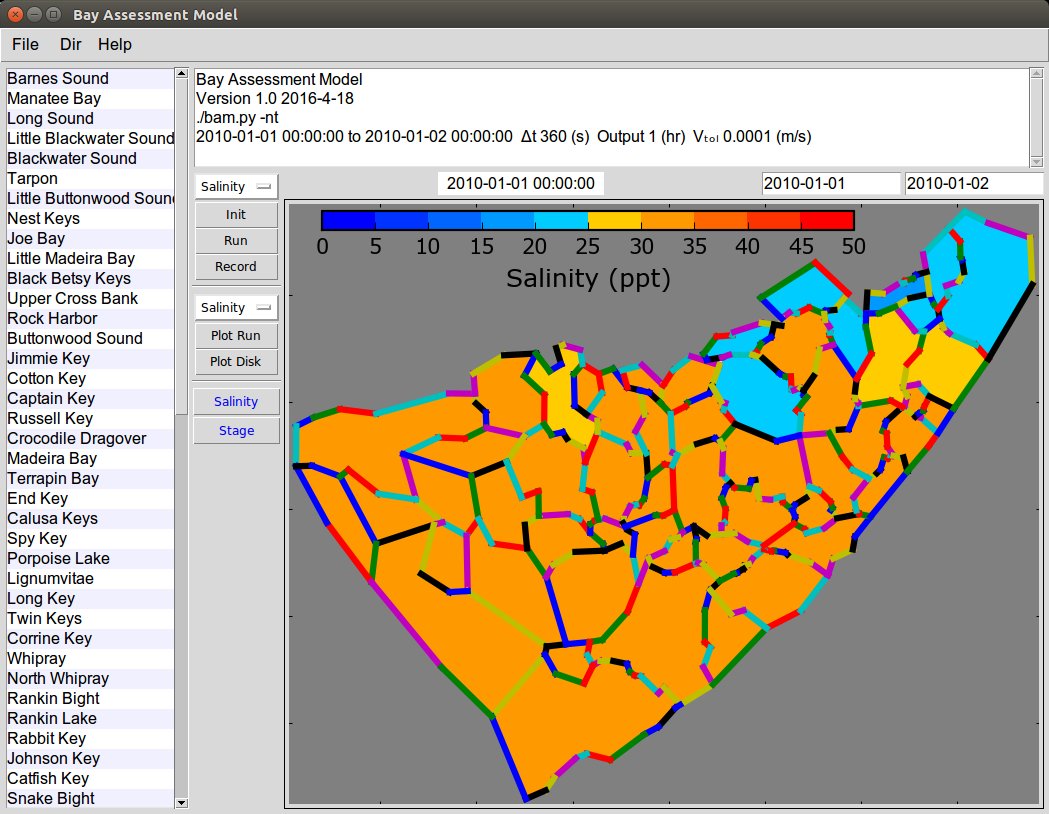
\includegraphics[ width = 0.9\textwidth ]{graphics/BAM_GUI.png}
  }
  {
     \caption{ \newline \newline BAM graphical user interface. }
     \label{fig:BAM_GUI}
  }
\end{figure}
%~~~~~~~~~~~~~~~~~~~~~~~~~~~~~~~~~~~~~~~~~

The main window is divided into 6 sections:
\begin{enumerate}
  %\itemsep-8pt
  \item Menu bar
  \item Basin listbox
  \item Message window
  \item Run and Plot controls
  \item Time display and entry boxes
  \item Map
\end{enumerate}
each described below. 

\clearpage 

%----------------------------------------------------------------
\subsection{Menu}
\label{sec:Menu}
%----------------------------------------------------------------
\subsubsection{File : Init}
The \texttt{File : Init} menu opens a dialogue box allowing the user to select a file to initialize basin variables.  The default is \texttt{Basin\_Initial\_Values.csv}.

\subsubsection{File : Edit}
\texttt{File : Edit} opens a dialogue box allowing the user to specify a file to be edited.  The editor which is invoked is specified with the \texttt{-e [--editor]} option (default: \texttt{gedit}). 

\subsubsection{Dir : Plot Disk}
The \texttt{Dir : Plot Disk} menu opens a dialogue box specifying the directory location of ouput data files to be plotted when the \texttt{Plot Disk} button is pressed.  The default is either the previous value of this dialogue selection, or the value of the \texttt{HOME} environment variable if defined, or the current working directory.

\subsubsection{Dir : Output}
\texttt{Dir : Output} opens a dialogue box specifying the directory location to write output data files.  The default is either the previous value of this dialogue selection, or the value of the \texttt{HOME} environment variable if defined, or the current working directory.

\clearpage
%----------------------------------------------------------------
\subsection{Basin listbox}
\label{sec:Basin listbox}
%----------------------------------------------------------------

%~~~~~~~~~~~~~~~~~~~~~~~~~~~~~~~~~~~~~~~~~
\begin{minipage}[t]{0.3\textwidth}
  \centering\raisebox{\dimexpr 0.6\baselineskip-\height}{
  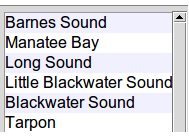
\includegraphics[width=\textwidth]{graphics/BasinListbox.png}}
\end{minipage}\hfill
\begin{minipage}[t]{0.65\textwidth}
The basin listbox allows the user to select any combination of basin objects with the mouse.  Single basins are also selected if clicked on the map.  When a basin is selected its current information is printed in the message window.  The basin listbox is also used to select basins for plot commands. 
\end{minipage}
%~~~~~~~~~~~~~~~~~~~~~~~~~~~~~~~~~~~~~~~~~

%----------------------------------------------------------------
\subsection{Run and Plot}
\label{sec:Run and Plot}
%----------------------------------------------------------------
These selectors and buttons control the map display and plotting options.

%~~~~~~~~~~~~~~~~~~~~~~~~~~~~~~~~~~~~~~~~~
\begin{minipage}[t]{0.25\textwidth}
  \centering\raisebox{\dimexpr 0.6\baselineskip-\height}{
  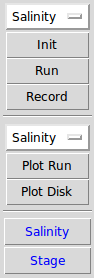
\includegraphics[width=\textwidth]{graphics/RunPlotControl.png}}
\end{minipage}\hfill
\begin{minipage}[t]{0.7\textwidth}
  \noindent
  
The top selector allows for either salinity or stage color graduations to be displayed on the map.\\

The \texttt{Init} button calls the model initialization function for the current model start, stop times and run options.\\

\texttt{Run} initiates model execution. \\

\texttt{Record} raises a pop-up window of check button selectors to specify which basin variables will be written to output.\\

The middle selector specifies the basin variable to be plotted. \\

\texttt{PlotRun} plots the currently selected variable from the model run for all basins selected in the basin list box.\\

\texttt{Plot Disk} plots the currently selected variable from the archive directory specified in the \texttt{Dir : Plot Disk} menu for all basins selected in the basin list box.\\

\texttt{Salinity} plots observed salinity data for basins selected in the basin list box where data is available.\\

\texttt{Stage} plots observed water level data for basins selected in the basin list box where data is available.
\end{minipage}
%~~~~~~~~~~~~~~~~~~~~~~~~~~~~~~~~~~~~~~~~~

%----------------------------------------------------------------
\subsection{Message window}
\label{sec:Message window}
%----------------------------------------------------------------
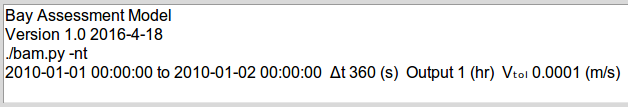
\includegraphics[width=0.7\textwidth]{graphics/MessageBox.png}

The message window is a text box displaying messages and information on model objects.  Messages generated during a model run are written to the \texttt{RunInfo.txt} file in the model output directory. 

%----------------------------------------------------------------
\subsection{Time}
\label{sec:Time}
%----------------------------------------------------------------

\includegraphics[width=0.7\textwidth]{graphics/TimeControl.png}

Current model time is displayed above the map in a message box. Two text entry boxes are located on the right above the map.  The text entry on the left can be used to set the model simulation start time, the text entry on the right to set the model simulation end time.

Simulation start and stop times can also be set with the \texttt{-S [--start]} and \texttt{-E [--end]} command line options.

Two formats are supported for time entry: \texttt{YYYY-MM-DD} and \texttt{YYYY-MM-DD HH:MM}.

%----------------------------------------------------------------
\subsection{Map}
\label{sec:Map}
%----------------------------------------------------------------
The map is an interactive display of two GIS shapefiles, the basins shapefile (\texttt{-bn [--basins]} default: \texttt{FLBayBasins}) and the shoals shapefile (\texttt{-s [--shoals]} default: \texttt{FathomLines}).

The map will display color graduations of basin state variables salinity or stage as specified with the selector (section \ref{sec:Run and Plot}). Shoals are shown with a random color assignment to allow easy visualization. 

Left-mouse-click on a basin will select the basin in the basin list box and will display current basin state variables in the message box.  Left-mouse-click on a shoal will display current shoal state variables in the message box. 

%~~~~~~~~~~~~~~~~~~~~~~~~~~~~~~~~~~~~~~~~~
\begin{minipage}[t]{0.25\textwidth}
  \centering\raisebox{\dimexpr 0.7\baselineskip-\height}{
  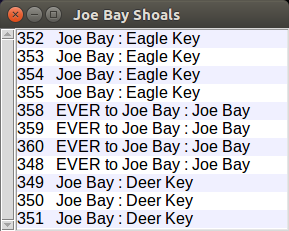
\includegraphics[width=\textwidth]{graphics/Shoal_ListBox.png}}
\end{minipage}\hfill
\begin{minipage}[t]{0.7\textwidth}
Right-mouse-click on a basin will present a list box with all shoals associated with the basin. Selecting a shoal in the list box will display current shoal state variables in the message box. 
\end{minipage}
%~~~~~~~~~~~~~~~~~~~~~~~~~~~~~~~~~~~~~~~~~ 

%----------------------------------------------------------------
%----------------------------------------------------------------
\clearpage 
\section{Mass Balance Check}
\label{sec:Mass Balance Check}
%----------------------------------------------------------------
%----------------------------------------------------------------
To check mass balance turn off all normal inputs and specify a fixed flow \newline (\texttt{-fb [--fixedBoundaryConditions]}) into Blue Bank with 1000 $\mathrm{m}^3$/s, t = 1 s timestep and all shoal Mannings coefficients of 0.1.  The \texttt{-bf [--basinFixedBCFile]} file would be:

\small
\begin{verbatim}
Basin, Name,      Type, Value
56,    Blue Bank, flow, 1000
\end{verbatim}
\large

The command line:

\small
\begin{verbatim}
./bam.py -t 1 -E "2010-1-1 08:00" -nt -nm -ne -nr -nR -nb -fb -si 'n' -sm 0.1
\end{verbatim}
\large

Blue Bank should then equilibriate at 8 hours to:

\small
\begin{verbatim}
    Blue Bank : dt = 1 s
      Stage: 0.01 (m)
      Salinity: 17.77 (g/kg)
      Volume: 0.0425 (km^3)
      Shoal Flux: 1000.0 (m^3/s)
\end{verbatim}
\large

Independent mass balance calculations and verification are detailed in \texttt{etc/Notes.txt}.


%----------------------------------------------------------------
%----------------------------------------------------------------
\clearpage 
\section{Salinity Check}
\label{sec:Salinty Check}
%----------------------------------------------------------------
%----------------------------------------------------------------
\small
\begin{verbatim}
------------------------------------------------------------------
Salinity Check: over 8:00 hours
Constant addition of V = 1000 m^3 to Blue Bank at dt = 60 s Manning 0.1
./bam.py -t 60 -nt -nm -ne -nr -nR -nb -fb -si 'n' -sm 0.1
Initial salinity in Blue Bank and surrounding basins is 35
------------------------------------------------------------------
Time     Salinity (ppt) Stage(m) Volume(m^3)  Flow(m^3/dt) Salt mass    Computed
2010-01-01 00    35.00  0        42277037     NA         1475257188737   35.00
2010-01-01 01    32.15  0.01     42501455     60275      1349060380152   31.84
2010-01-01 02    29.54  0.01     42501891     60293      1234233094273   29.13
2010-01-01 03    27.14  0.01     42501966     60294      1129178205339   26.65
2010-01-01 04    24.94  0.01     42501989     60295      1033064976498   24.38
2010-01-01 05    22.91  0.01     42501995     60295       945132604037   22.30
2010-01-01 06    21.05  0.01     42501998     60295       864684834211   20.41
2010-01-01 07    19.34  0.01     42501999     60295       791084610753   18.67
2010-01-01 08    17.77  0.01     42501999     60295       723749088579   17.08
						
Timesteps per Interval (hour) 60
\end{verbatim}
\large

The above BAM reported values are correct, the Salt mass and Computed salinity are from a spreadsheet. The Computed salinity is inaccurate due to inaccurate volume and salt mass computations at a timestep of 60 seconds.  

Salinity verification at t = 1s can be found in \texttt{etc/BlueBankSalinity-Q+1000cms\_dt1.ods}, and is reproduced below:

\small
\begin{verbatim}
Time               Salinity(ppt) Stage(m) Volume(m^3)  Flow(m^3/dt)  Salt mass  Computed
2010-01-01 00:00:00     35           0  42277036.502    NA       1475257188737  35.00
2010-01-01 00:00:01     34.999       0  42278036.502    0        1475257188737  35.00
2010-01-01 00:00:02     34.998       0  42278968.321    68.182   1475254809583  35.00
2010-01-01 00:00:03     34.998       0  42279873.768    94.553   1475251510312  35.00
2010-01-01 00:00:04     34.997       0  42280759.225    114.543  1475247513617  35.00
...
2010-01-01 07:59:56     17.774    0.01  42500628.472    1000      753148504363  17.77
2010-01-01 07:59:57     17.774    0.01  42500628.472    1000      753130783484  17.77
2010-01-01 07:59:58     17.773    0.01  42500628.472    1000      753113063021  17.77
2010-01-01 07:59:59     17.773    0.01  42500628.472    1000      753095342976  17.77
2010-01-01 08:00:00     17.773    0.01  42500628.472    1000      753077623348  17.77
\end{verbatim}
\large

%----------------------------------------------------------------
%----------------------------------------------------------------
\clearpage 
\section{Runoff Calibration}
\label{sec:Runoff Calibration}
%----------------------------------------------------------------
%----------------------------------------------------------------
Runoff from the Everglades to coastal basins is determined by the relative water level elevation between the Everglades and coastal basins.  This allows for both positive and negative runoff between the Everglades and coastal basins.  Shoal properties of the coastal basins (length, width, depth) have been calibrated to match aggregate runoff from the FATHOM model \citep{Cosby2010} over the rainy seasons of 2001, 2002 and 2003, the three years of overlap between BAM and FATHOM.  Plots shown below compare the calibrated basin runoff and FATHOM values. It should be noted that FATHOM values are strictly negative (no flow is allowed from the coastal basins into the Everglades) and are available at only 1 point per month. \\[-1cm]

%~~~~~~~~~~~~~~~~~~~~~~~~~~~~~~~~~~~~~~~~~
\begin{figure}[H]
  \subfloat[Barnes Sound 2000-05-01]{
    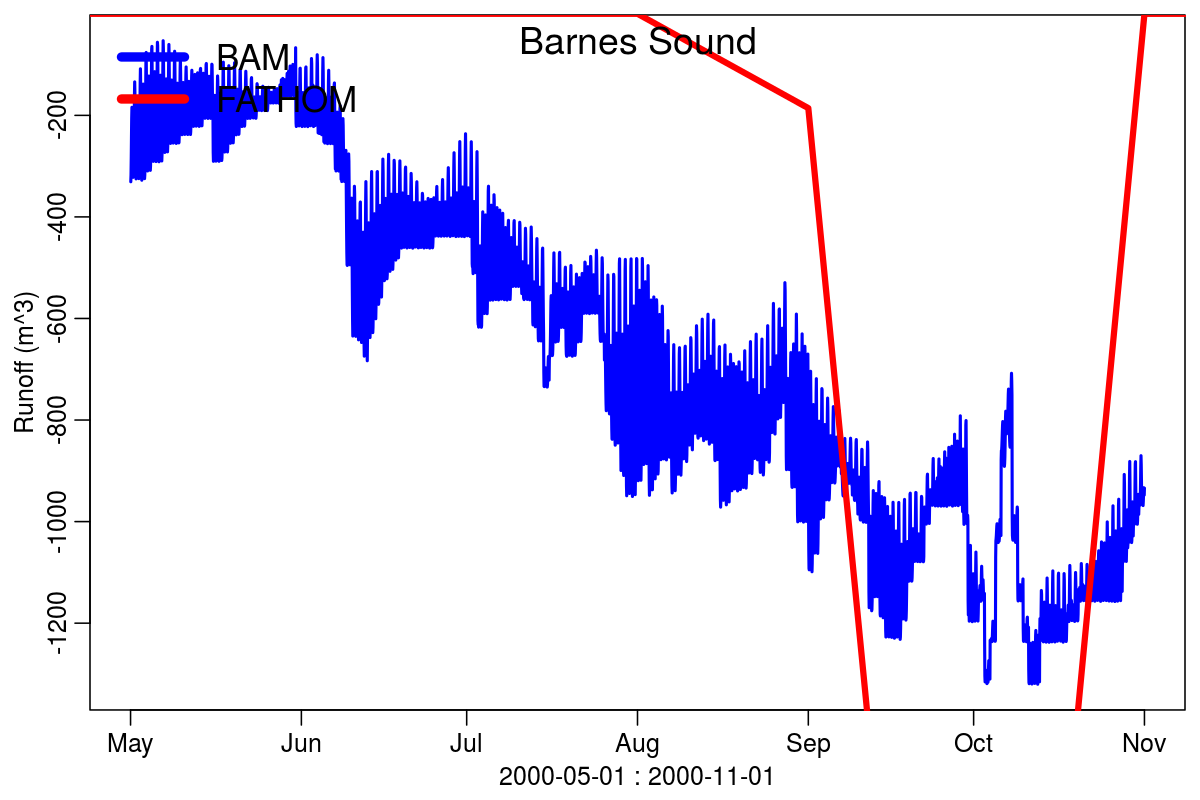
\includegraphics[ width = 0.4\textwidth ]{graphics/RunoffCompare/Barnes Sound 2000-05-01 Runoff.png}
  }
  \subfloat[Manatee Bay 2000-05-01]{
    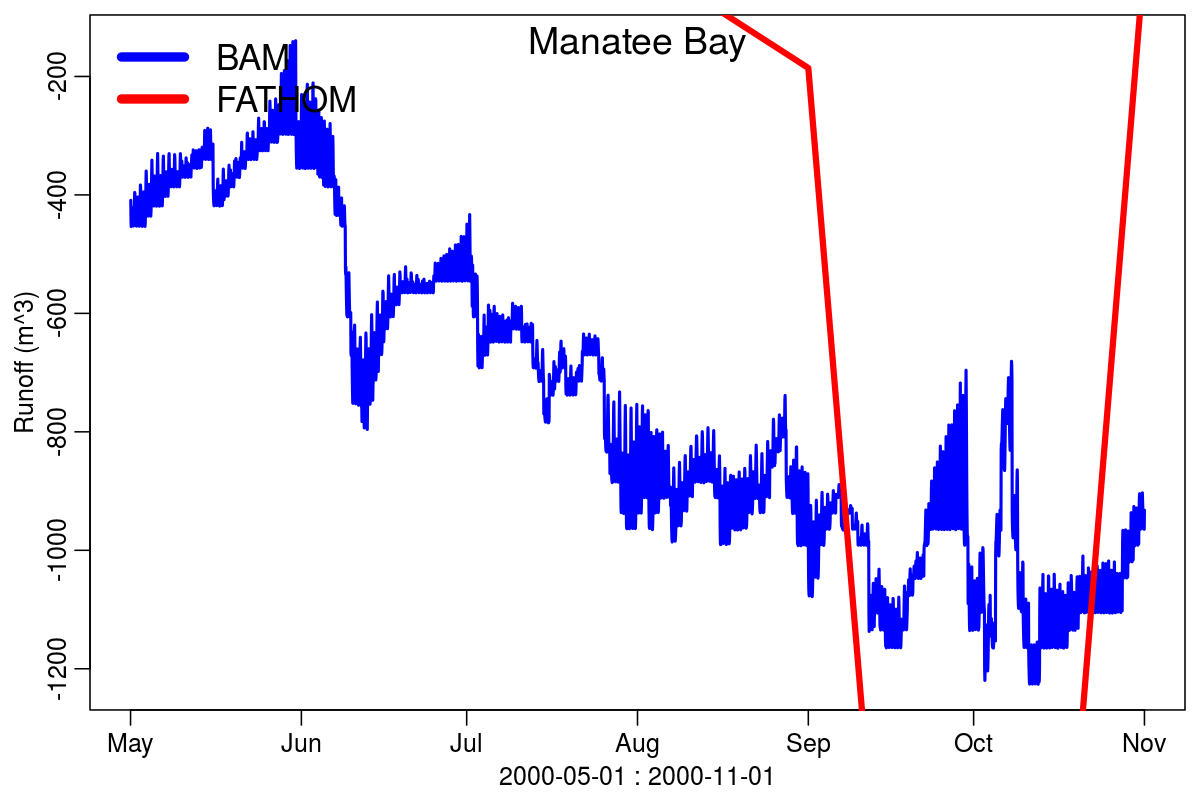
\includegraphics[ width = 0.4\textwidth ]{graphics/RunoffCompare/Manatee Bay 2000-05-01 Runoff.png}
  }
  
  \subfloat[Barnes Sound 2001-05-01]{
    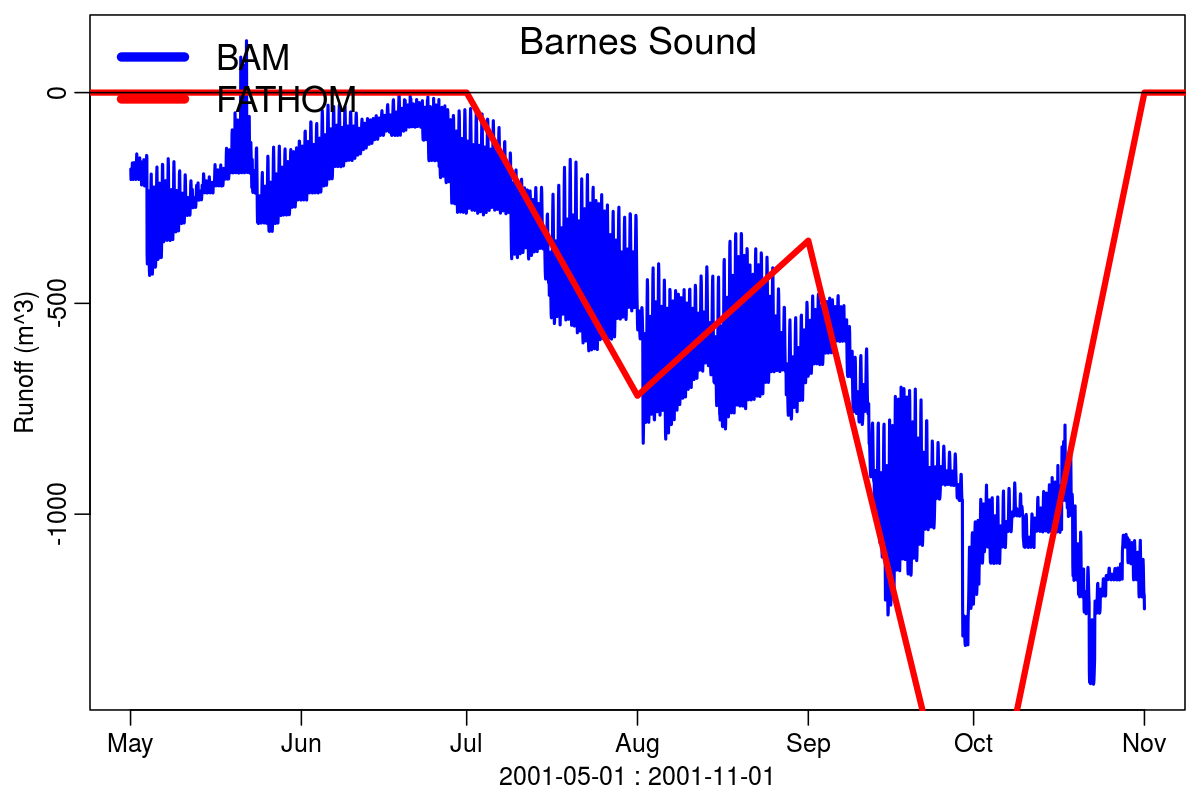
\includegraphics[ width = 0.4\textwidth ]{graphics/RunoffCompare/Barnes Sound 2001-05-01 Runoff.png}
  }
  \subfloat[Manatee Bay 2001-05-01]{
    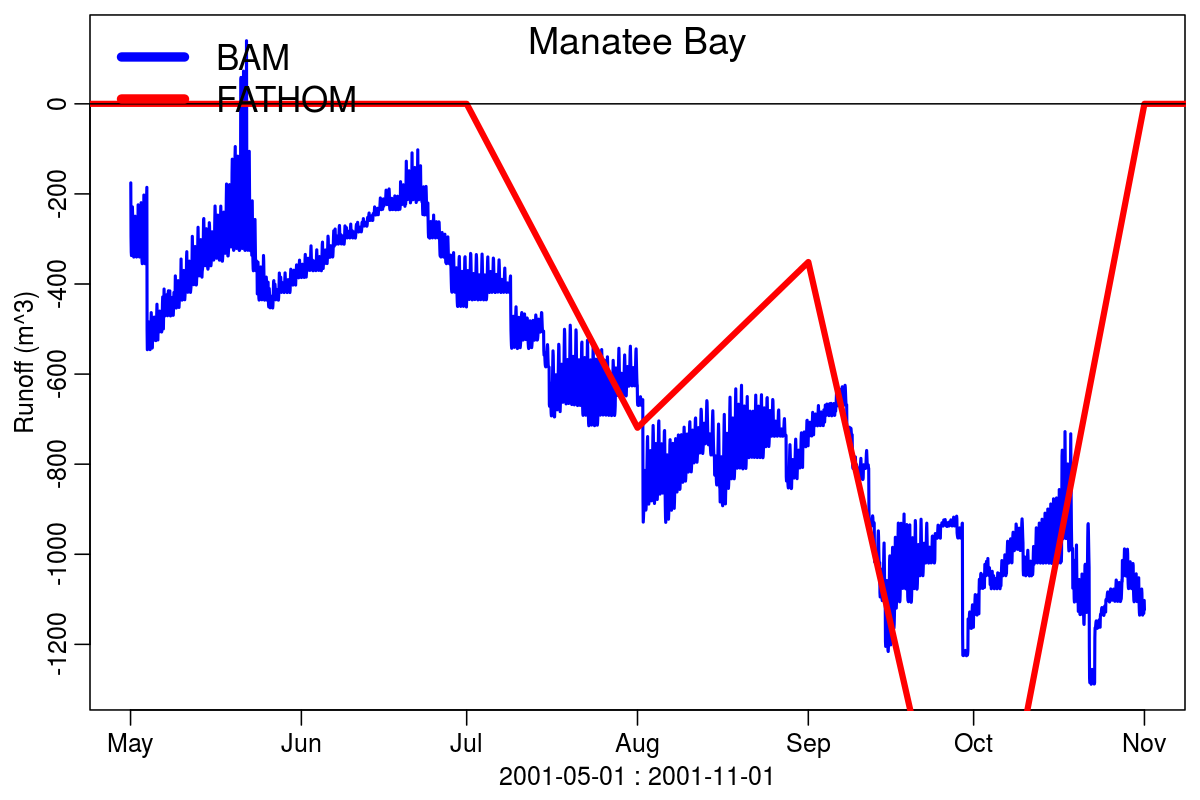
\includegraphics[ width = 0.4\textwidth ]{graphics/RunoffCompare/Manatee Bay 2001-05-01 Runoff.png}
  }

  \subfloat[Barnes Sound 2002-05-01]{
    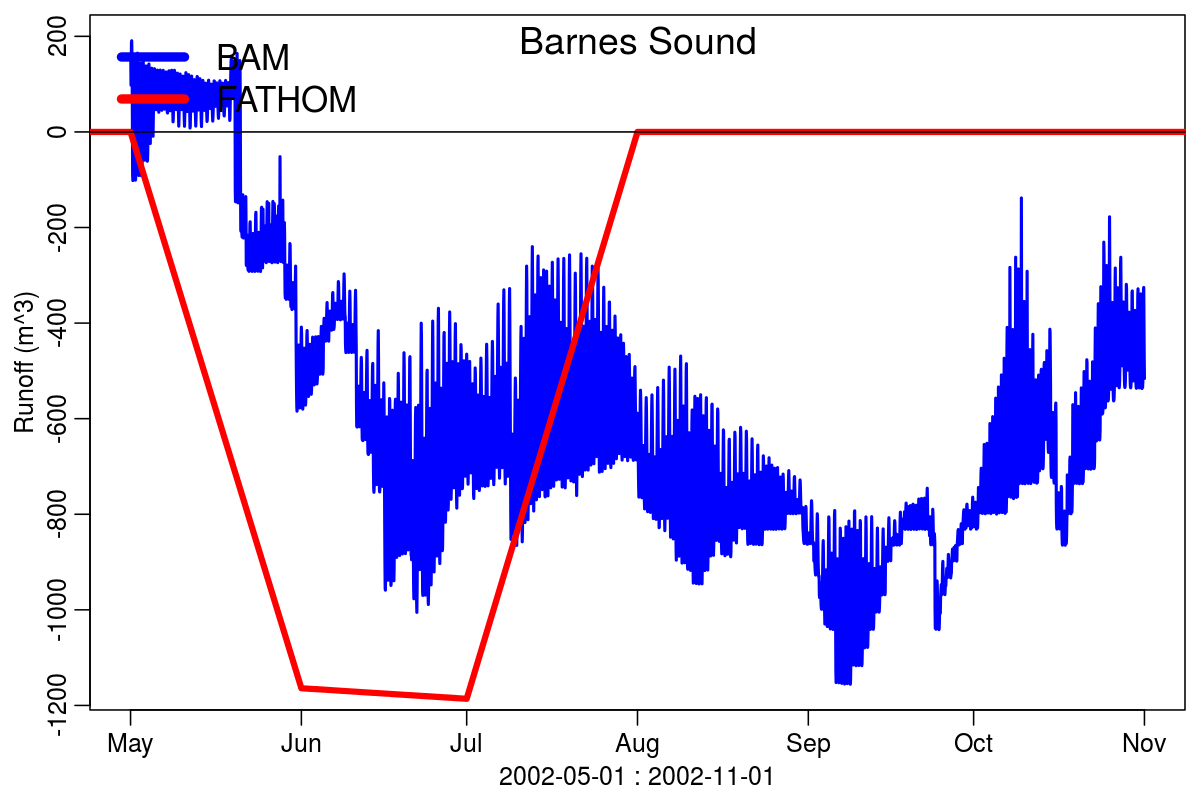
\includegraphics[ width = 0.4\textwidth ]{graphics/RunoffCompare/Barnes Sound 2002-05-01 Runoff.png}
  }
  \subfloat[Manatee Bay 2002-05-01]{
    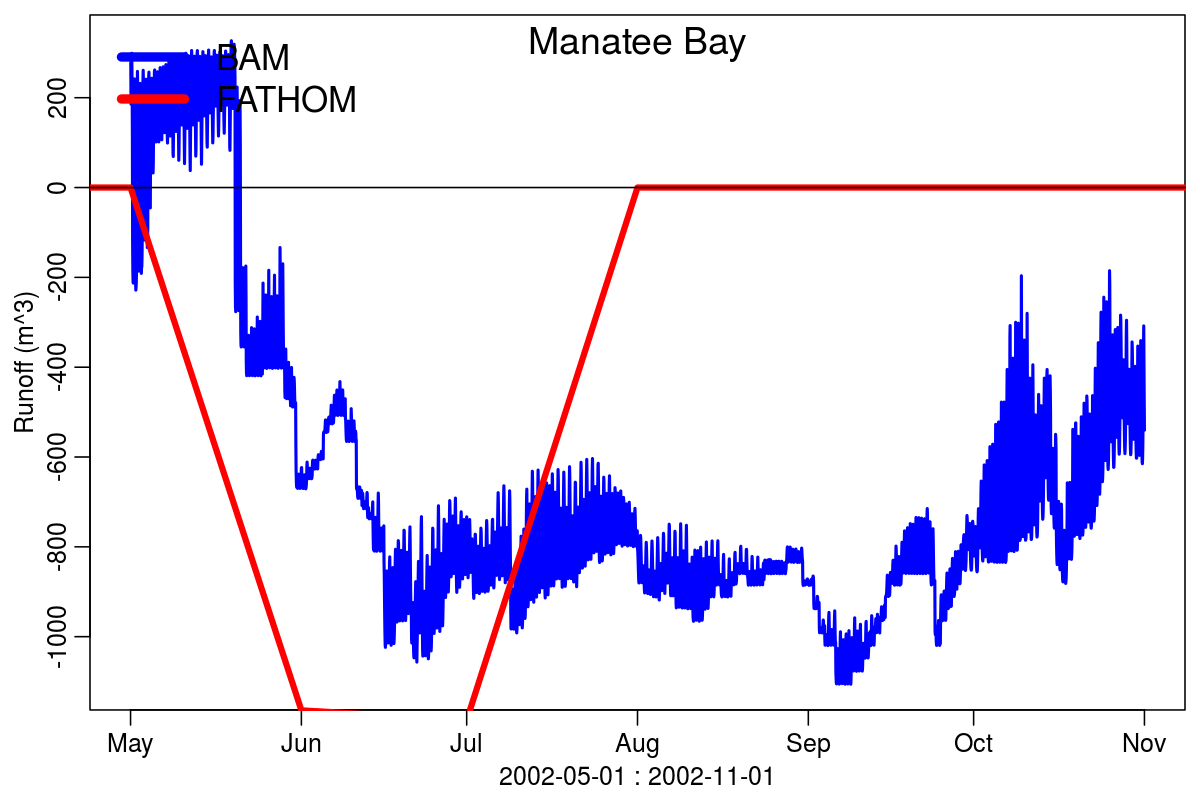
\includegraphics[ width = 0.4\textwidth ]{graphics/RunoffCompare/Manatee Bay 2002-05-01 Runoff.png}
  }
  \caption{Barnes Sound and Manatee Bay Runoff}
  \label{fig:Barnes Sound and Manatee Bay Runoff}
\end{figure}
%~~~~~~~~~~~~~~~~~~~~~~~~~~~~~~~~~~~~~~~~~

%~~~~~~~~~~~~~~~~~~~~~~~~~~~~~~~~~~~~~~~~~
\begin{figure}[H]
  \subfloat[2000-05-01]{
    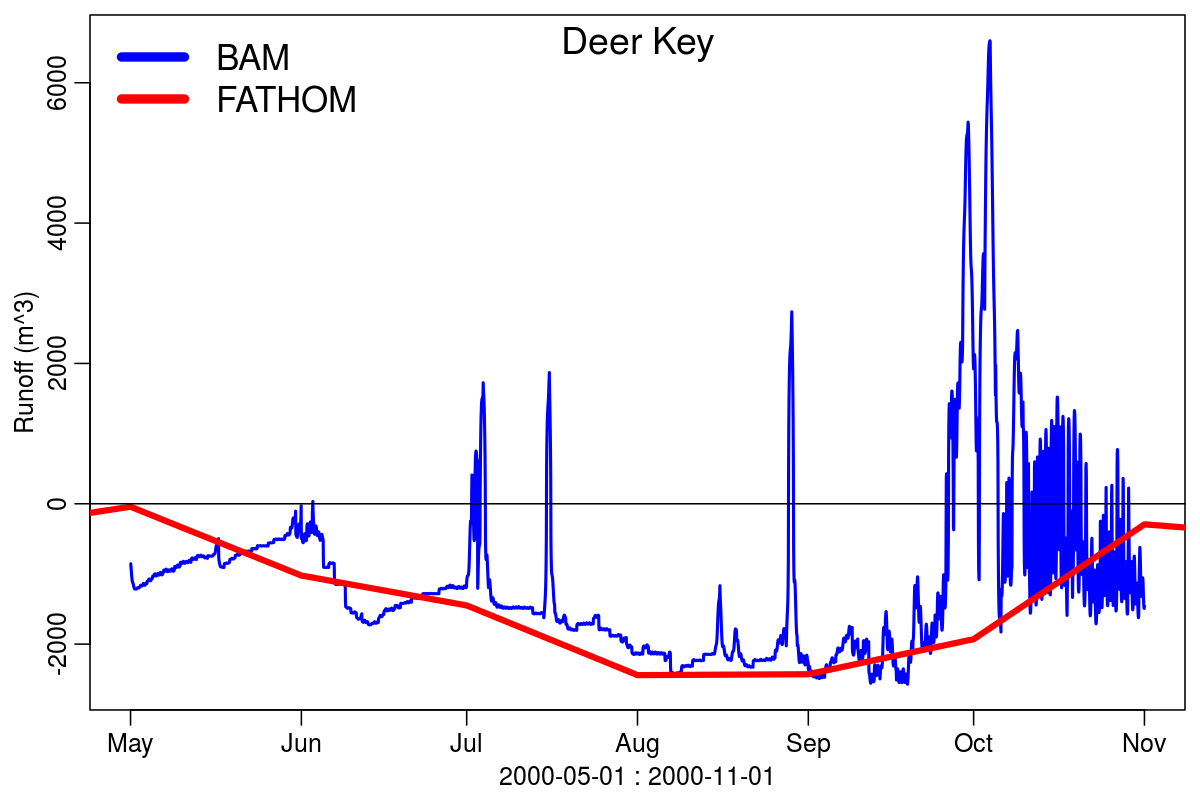
\includegraphics[ width = 0.5\textwidth ]{graphics/RunoffCompare/Deer Key 2000-05-01 Runoff.png}
  }
  \subfloat[2000-05-01]{
    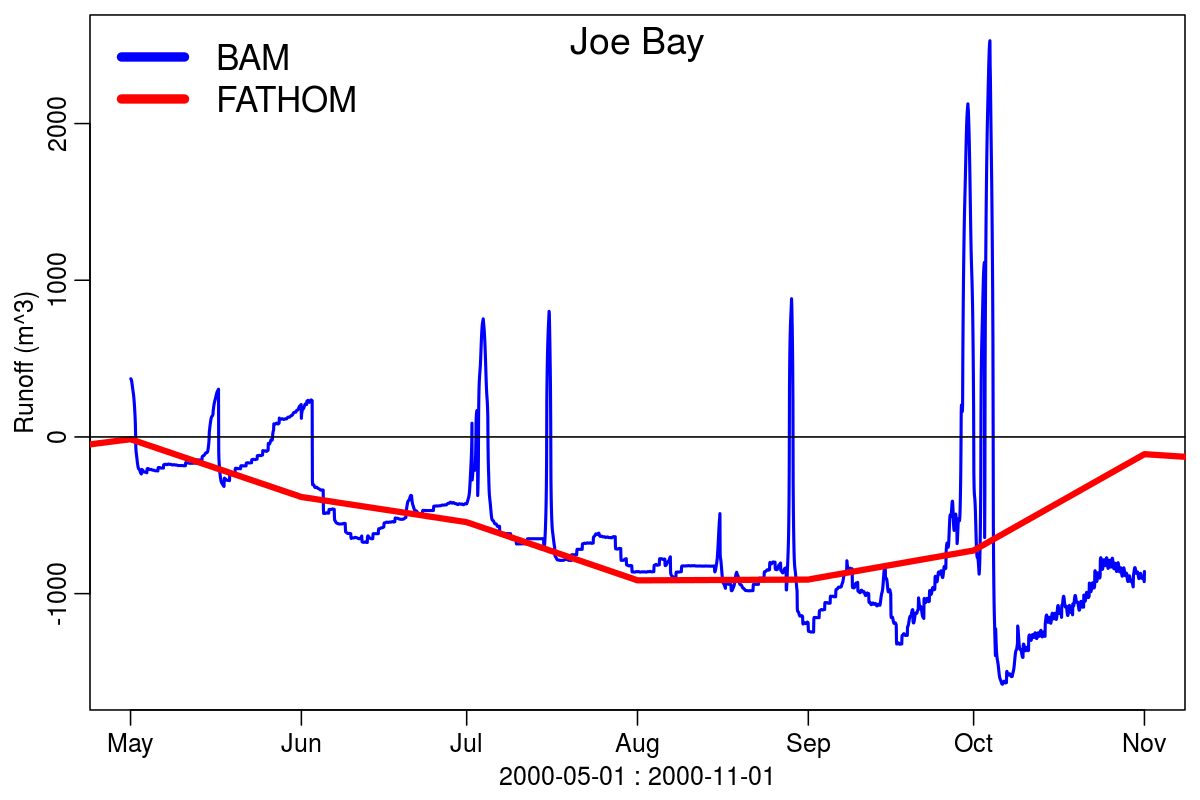
\includegraphics[ width = 0.5\textwidth ]{graphics/RunoffCompare/Joe Bay 2000-05-01 Runoff.png}
  }
  
  \subfloat[2001-05-01]{
    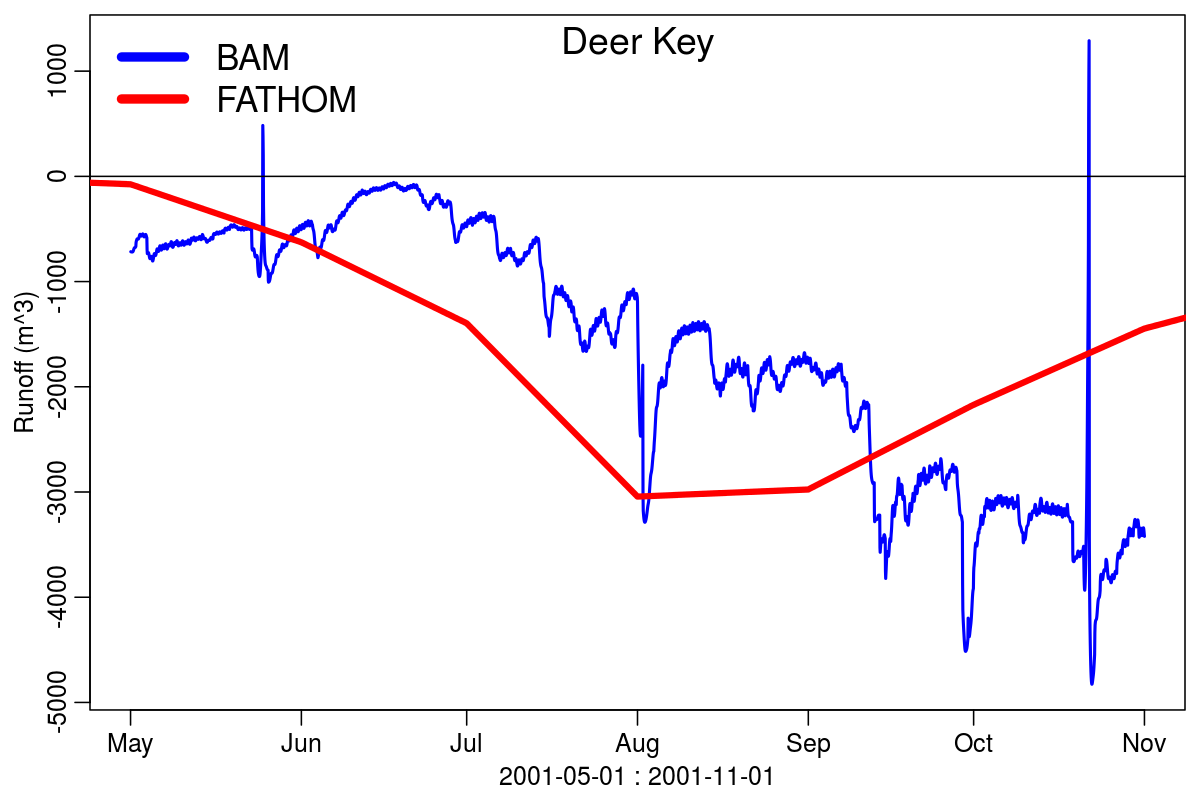
\includegraphics[ width = 0.5\textwidth ]{graphics/RunoffCompare/Deer Key 2001-05-01 Runoff.png}
  }
  \subfloat[2001-05-01]{
    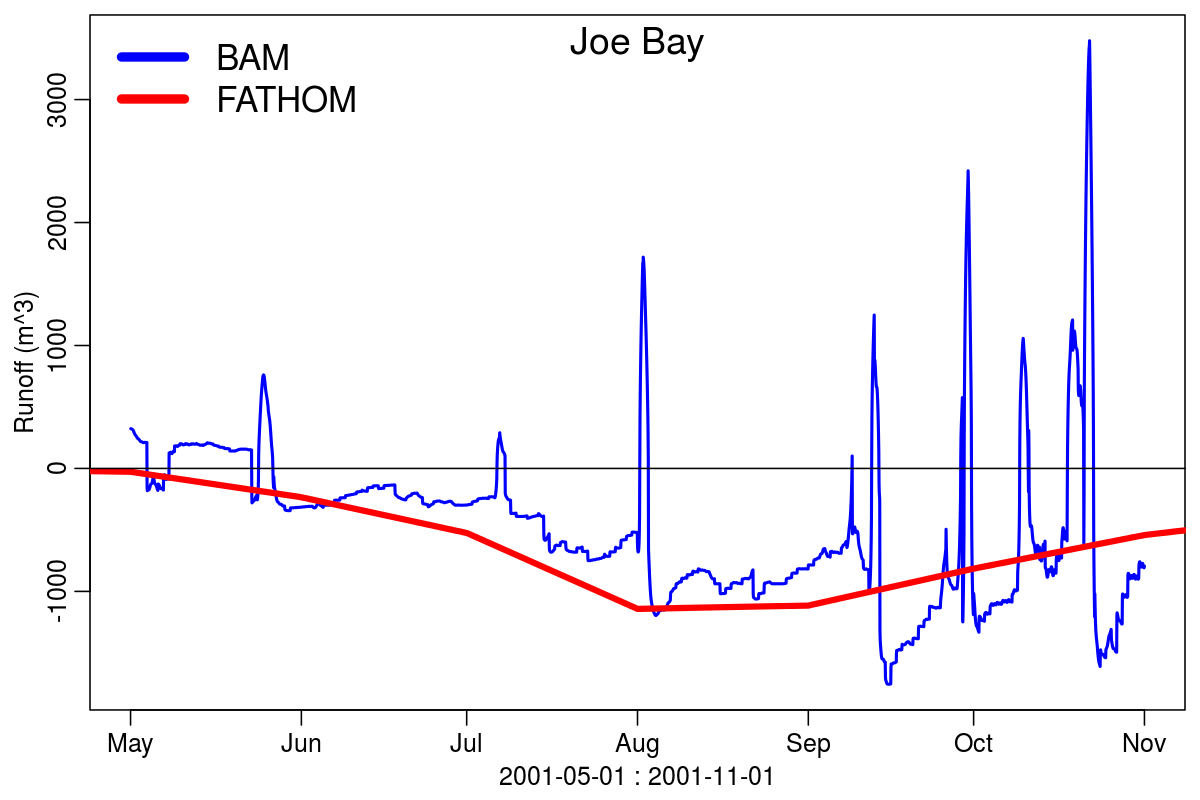
\includegraphics[ width = 0.5\textwidth ]{graphics/RunoffCompare/Joe Bay 2001-05-01 Runoff.png}
  }
  
  \subfloat[2002-05-01]{
    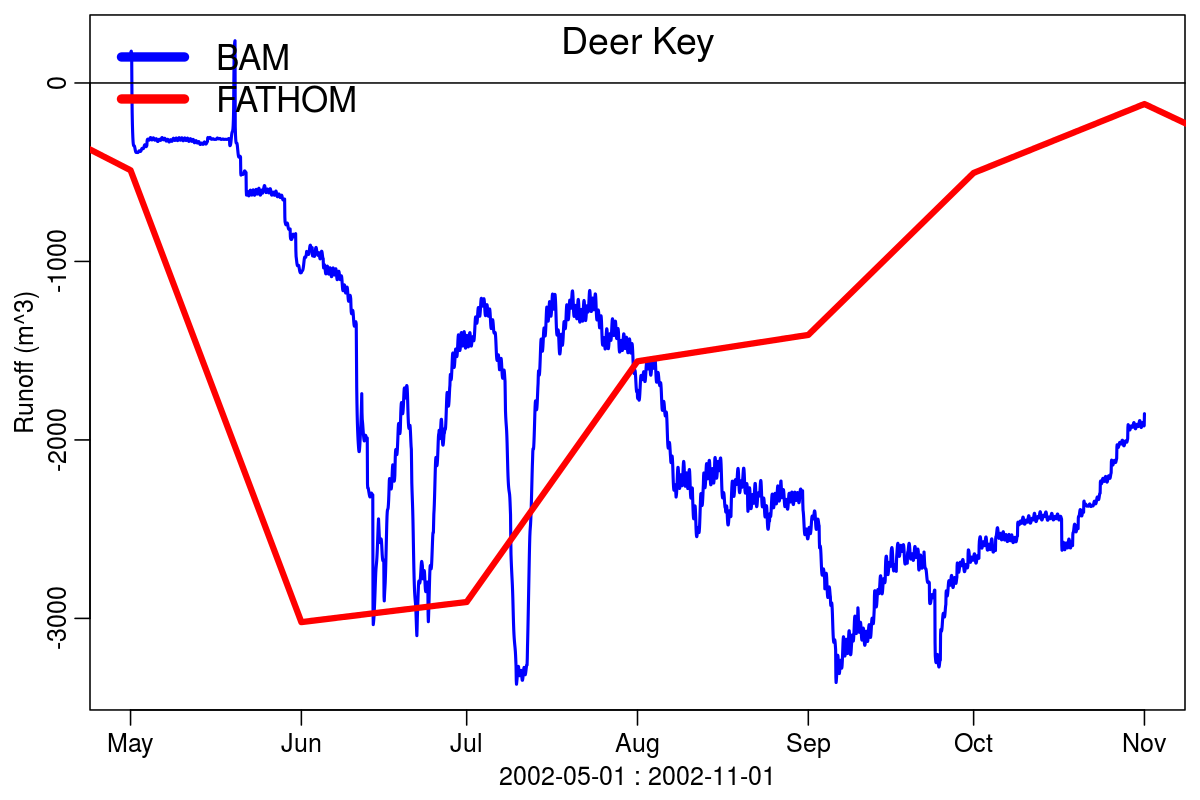
\includegraphics[ width = 0.5\textwidth ]{graphics/RunoffCompare/Deer Key 2002-05-01 Runoff.png}
  }
  \subfloat[2002-05-01]{
    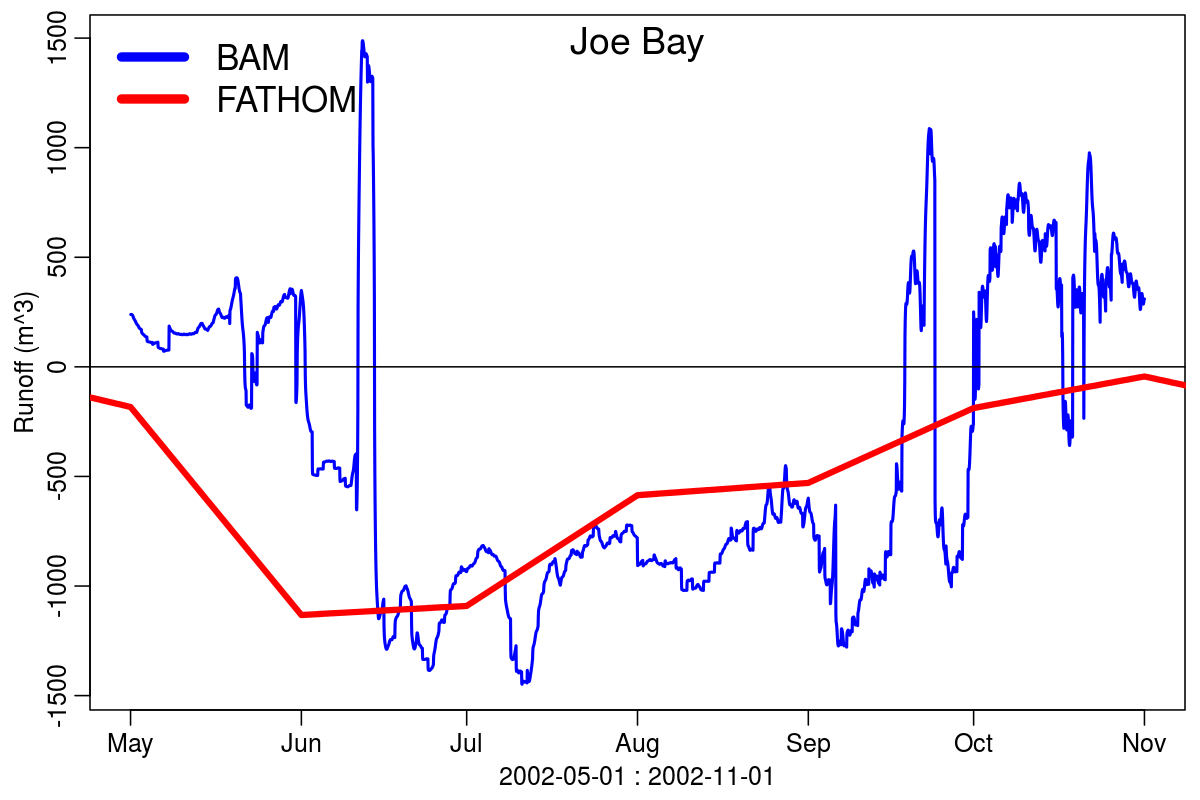
\includegraphics[ width = 0.5\textwidth ]{graphics/RunoffCompare/Joe Bay 2002-05-01 Runoff.png}
  }
   \caption{Deer Key and Joe Bay Runoff}
  \label{fig:Deer Key and Joe Bay Runoff}
\end{figure}
%~~~~~~~~~~~~~~~~~~~~~~~~~~~~~~~~~~~~~~~~~

%~~~~~~~~~~~~~~~~~~~~~~~~~~~~~~~~~~~~~~~~~
\begin{figure}[H]
  \subfloat[2000-05-01]{
    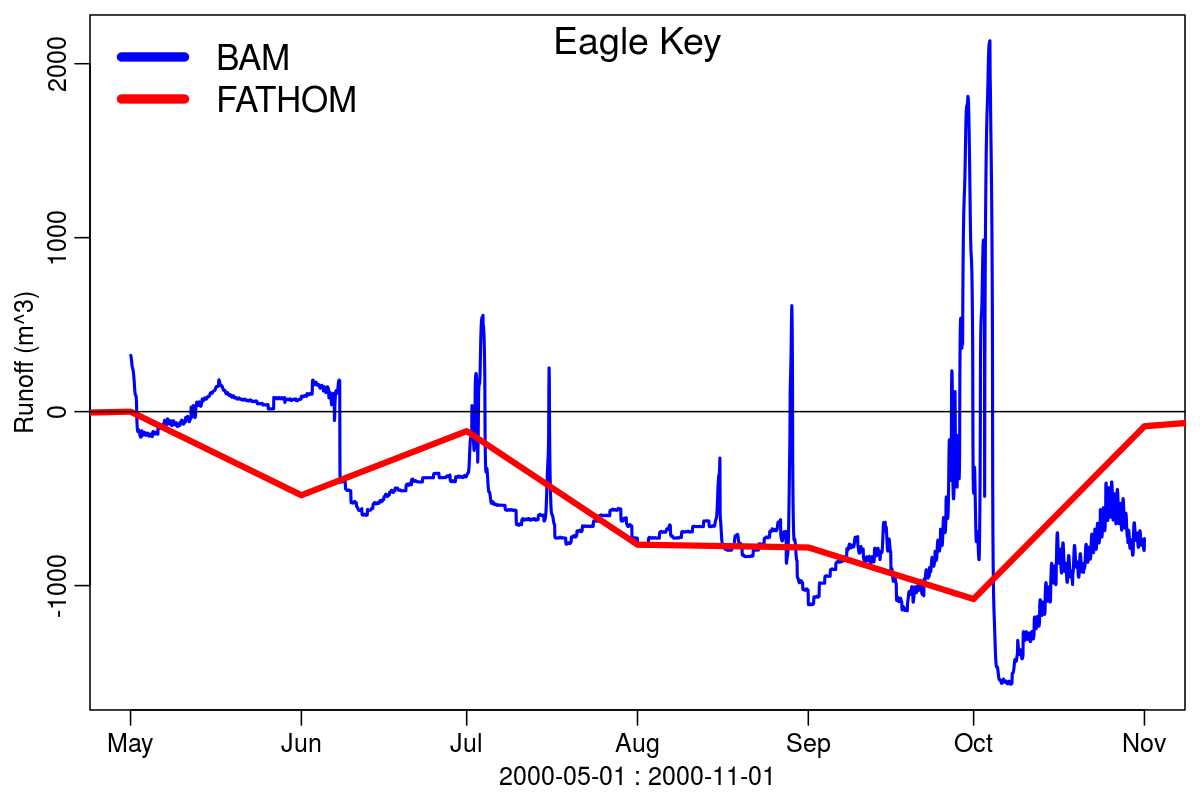
\includegraphics[ width = 0.5\textwidth ]{graphics/RunoffCompare/Eagle Key 2000-05-01 Runoff.png}
  }
  \subfloat[2000-05-01]{
    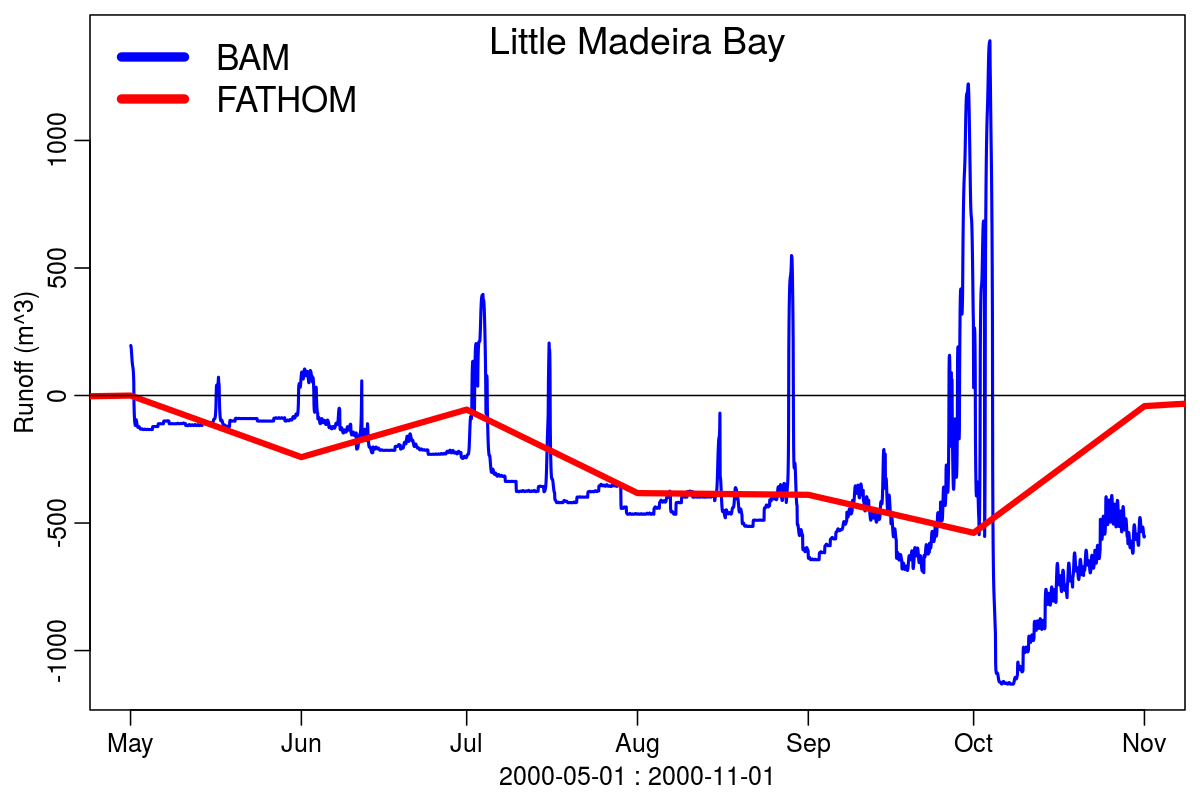
\includegraphics[ width = 0.5\textwidth ]{graphics/RunoffCompare/Little Madeira Bay 2000-05-01 Runoff.png}
  }
  
  \subfloat[2001-05-01]{
    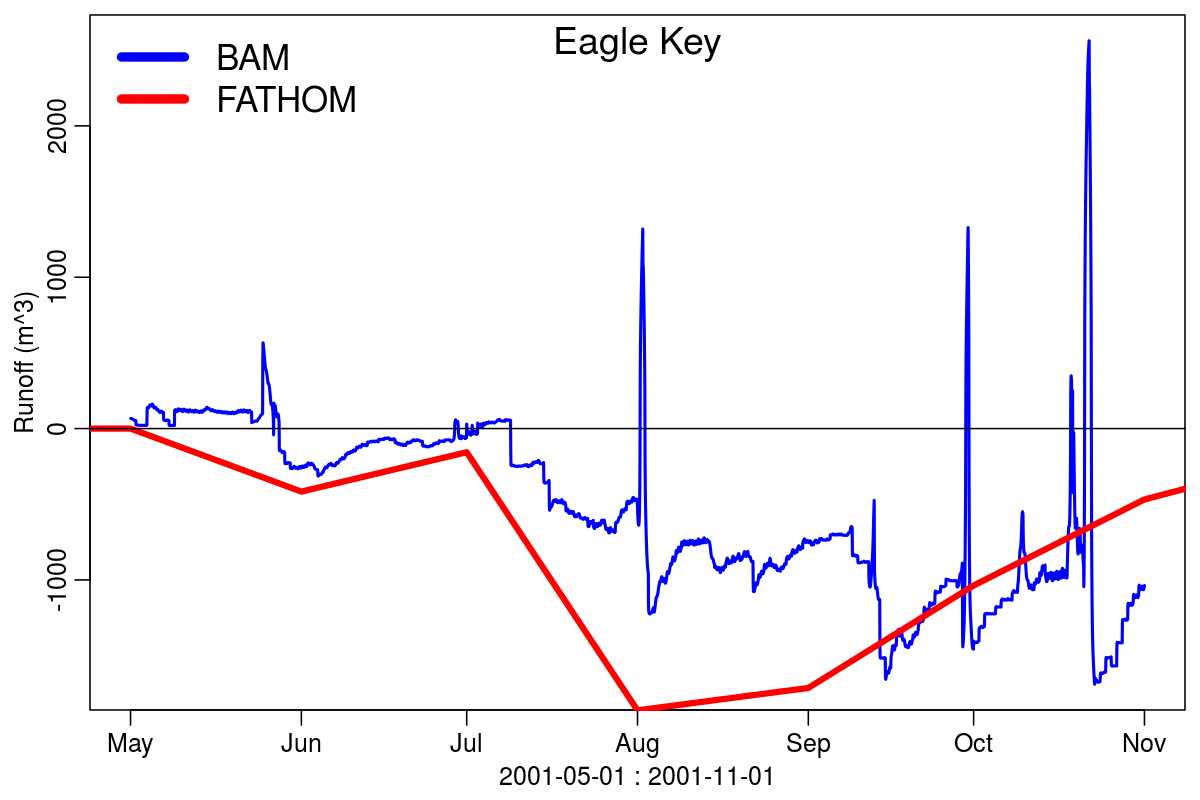
\includegraphics[ width = 0.5\textwidth ]{graphics/RunoffCompare/Eagle Key 2001-05-01 Runoff.png}
  }
  \subfloat[2001-05-01]{
    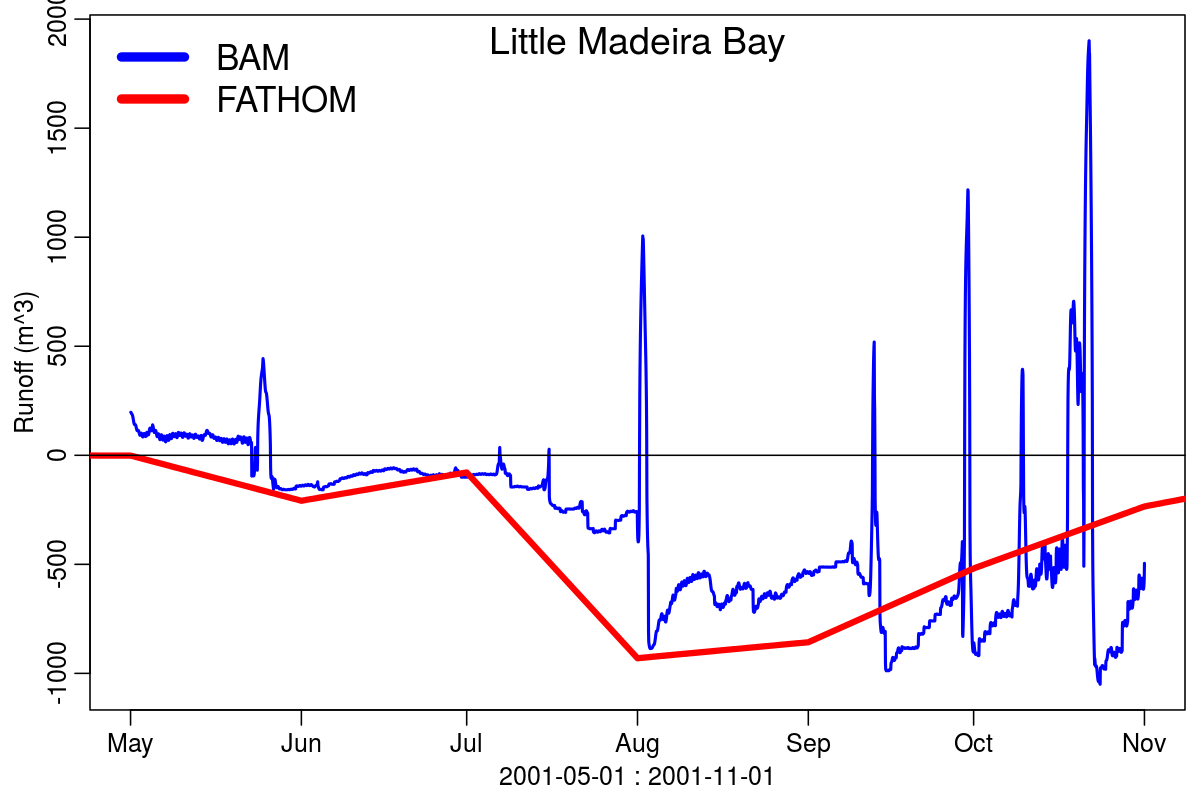
\includegraphics[ width = 0.5\textwidth ]{graphics/RunoffCompare/Little Madeira Bay 2001-05-01 Runoff.png}
  }

  \subfloat[2002-05-01]{
    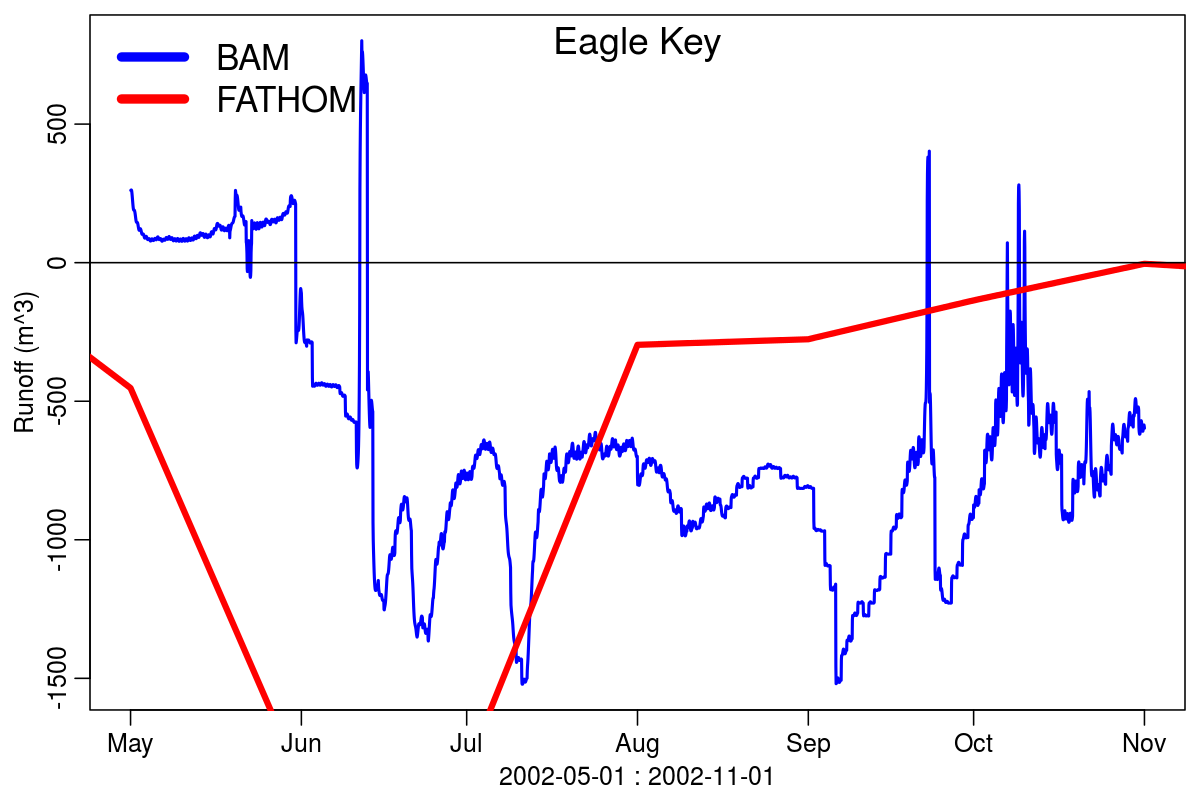
\includegraphics[ width = 0.5\textwidth ]{graphics/RunoffCompare/Eagle Key 2002-05-01 Runoff.png}
  }
  \subfloat[2002-05-01]{
    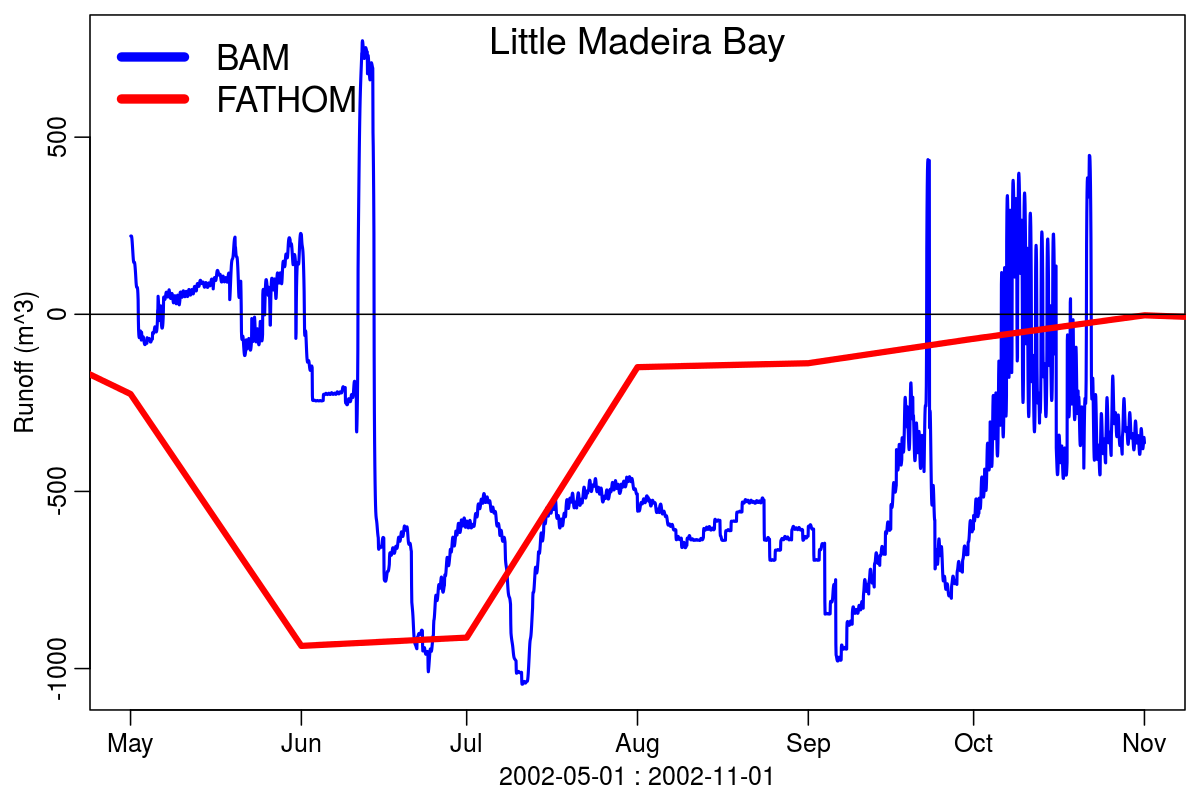
\includegraphics[ width = 0.5\textwidth ]{graphics/RunoffCompare/Little Madeira Bay 2002-05-01 Runoff.png}
  }
  \caption{Eagle Key and Little Madeira Bay Runoff}
  \label{fig:Eagle Key and Little Madeira Bay Runoff}
\end{figure}
%~~~~~~~~~~~~~~~~~~~~~~~~~~~~~~~~~~~~~~~~~


%~~~~~~~~~~~~~~~~~~~~~~~~~~~~~~~~~~~~~~~~~
\begin{figure}[H]
  \subfloat[2000-05-01]{
    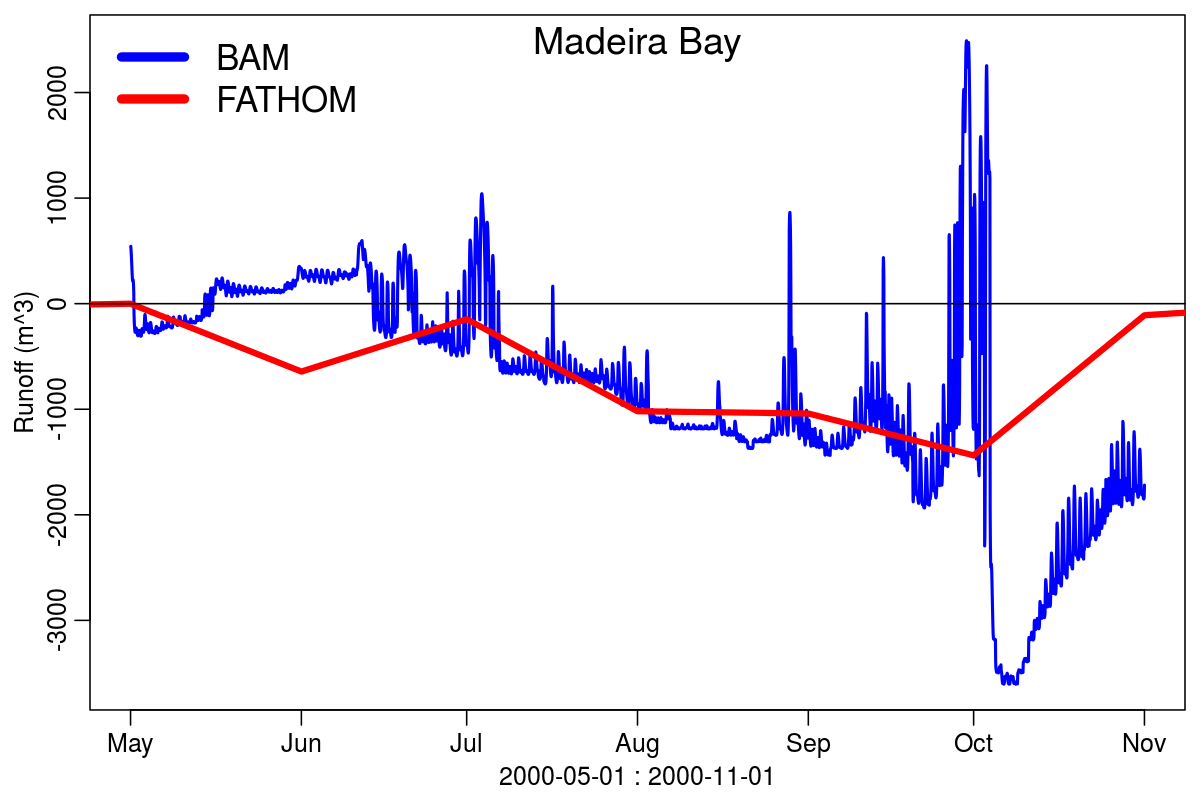
\includegraphics[ width = 0.5\textwidth ]{graphics/RunoffCompare/Madeira Bay 2000-05-01 Runoff.png}
  }
  \subfloat[2000-05-01]{
    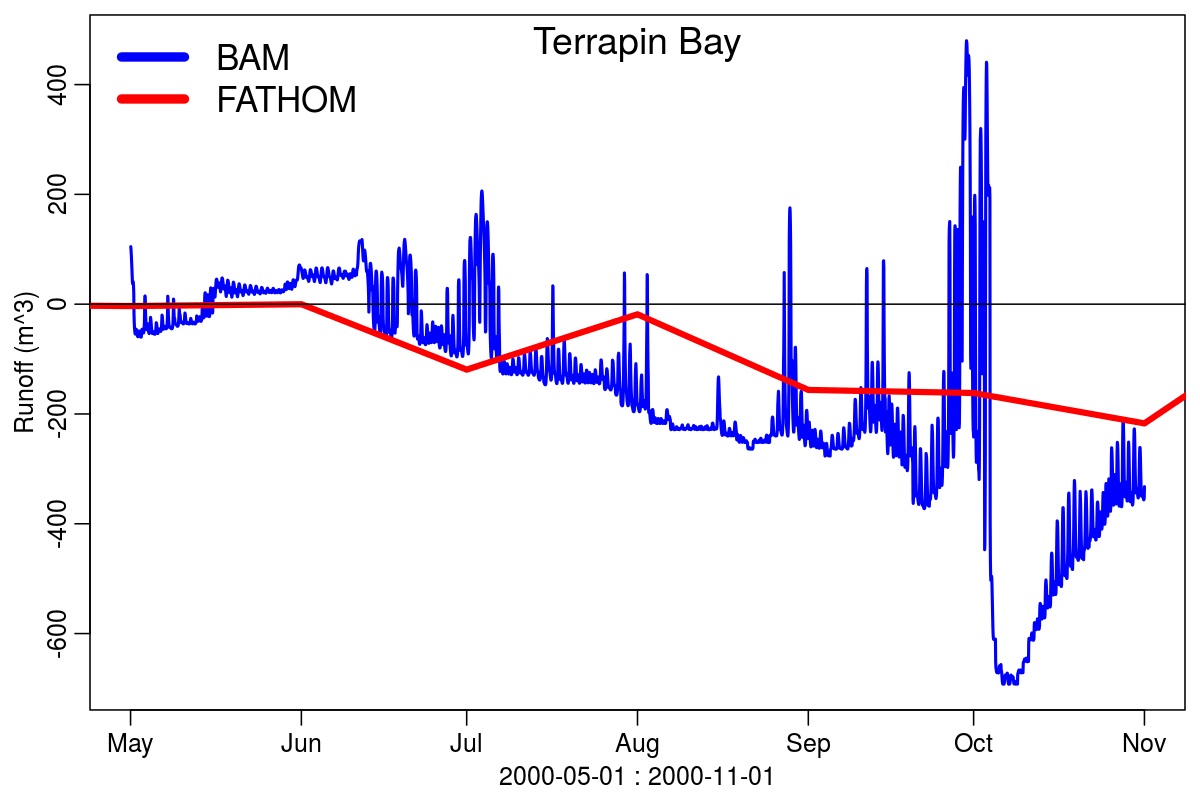
\includegraphics[ width = 0.5\textwidth ]{graphics/RunoffCompare/Terrapin Bay 2000-05-01 Runoff.png}
  }
  
  \subfloat[2001-05-01]{
    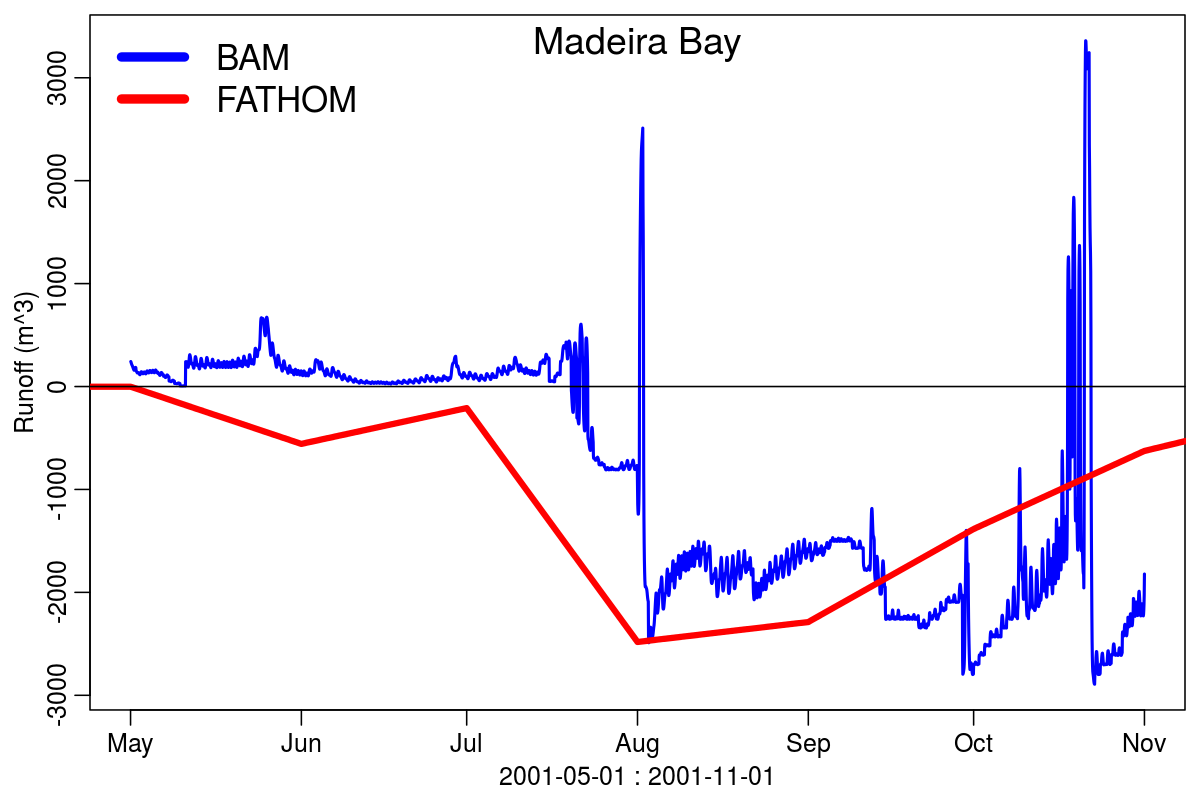
\includegraphics[ width = 0.5\textwidth ]{graphics/RunoffCompare/Madeira Bay 2001-05-01 Runoff.png}
  }
  \subfloat[2001-05-01]{
    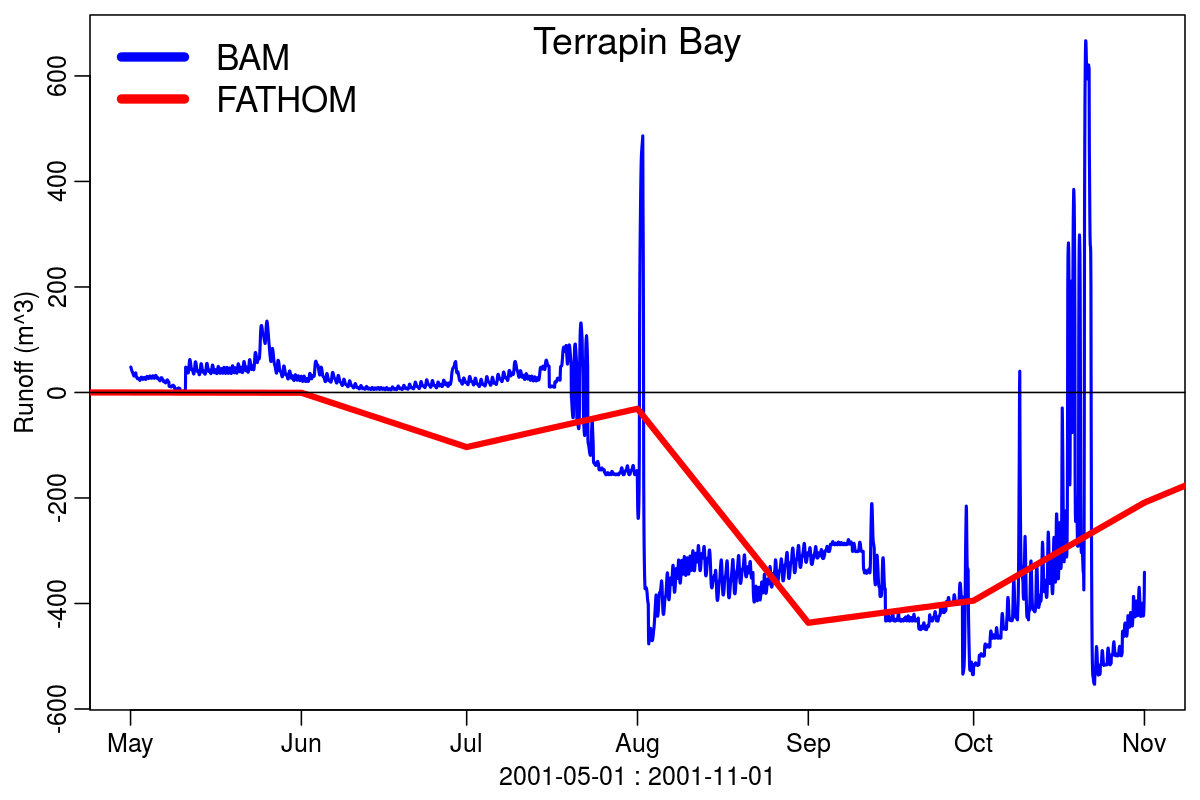
\includegraphics[ width = 0.5\textwidth ]{graphics/RunoffCompare/Terrapin Bay 2001-05-01 Runoff.png}
  }

  \subfloat[2002-05-01]{
    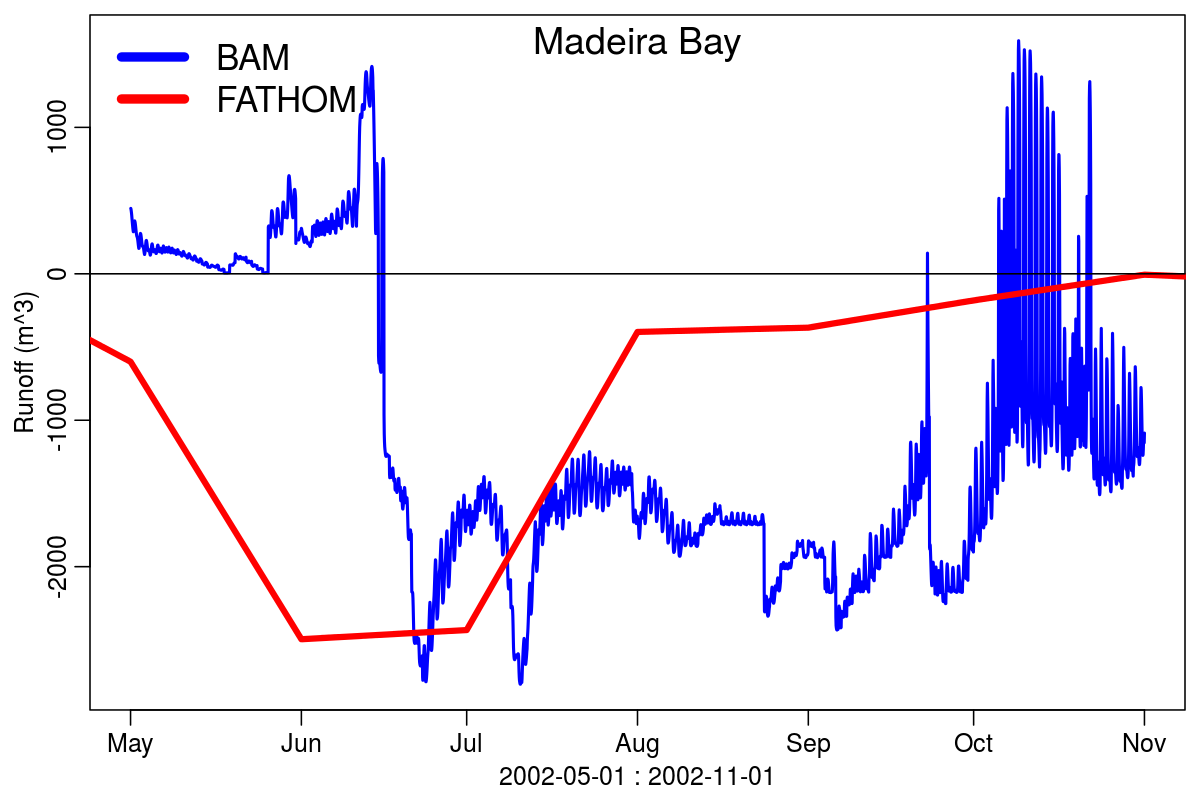
\includegraphics[ width = 0.5\textwidth ]{graphics/RunoffCompare/Madeira Bay 2002-05-01 Runoff.png}
  }
  \subfloat[2002-05-01]{
    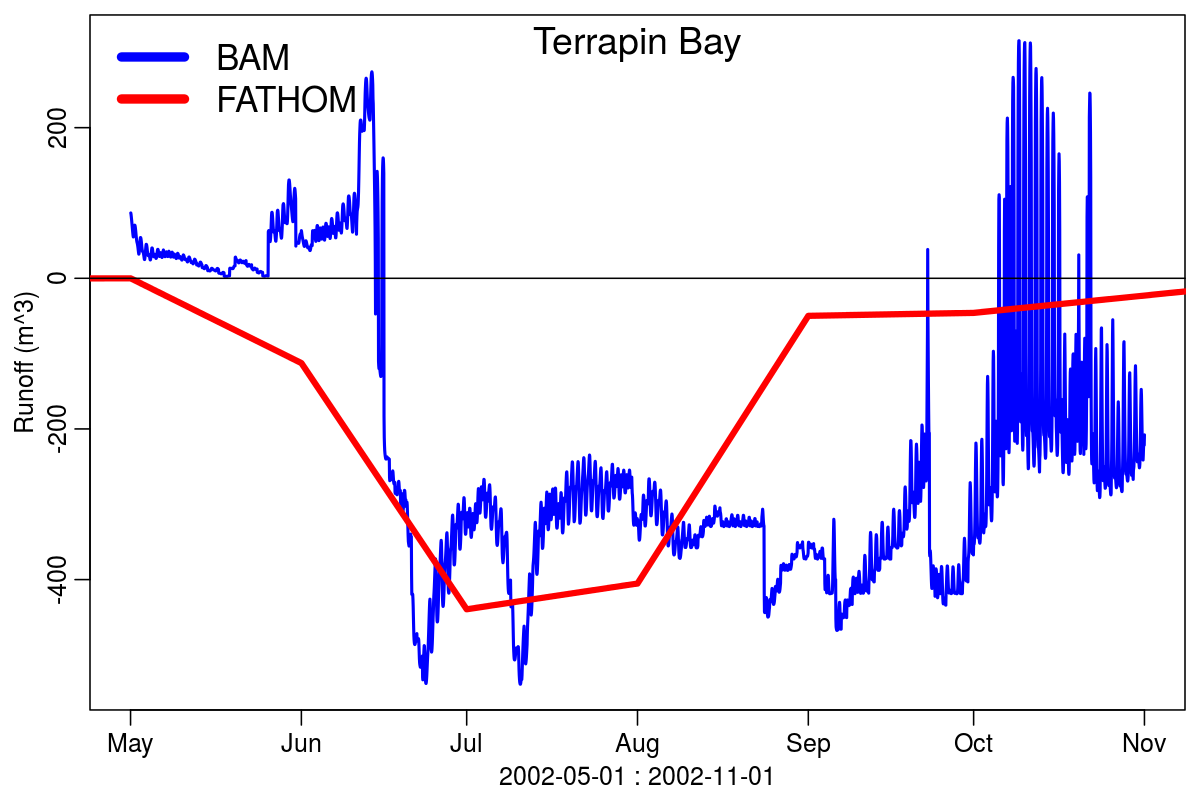
\includegraphics[ width = 0.5\textwidth ]{graphics/RunoffCompare/Terrapin Bay 2002-05-01 Runoff.png}
  }
  \caption{Madeira Bay and Terrapin Bay Runoff}
  \label{fig:Madeira Bay and Terrapin Bay Runoff}
\end{figure}
%~~~~~~~~~~~~~~~~~~~~~~~~~~~~~~~~~~~~~~~~~

%~~~~~~~~~~~~~~~~~~~~~~~~~~~~~~~~~~~~~~~~~
\begin{figure}[H]
  \subfloat[2000-05-01]{
    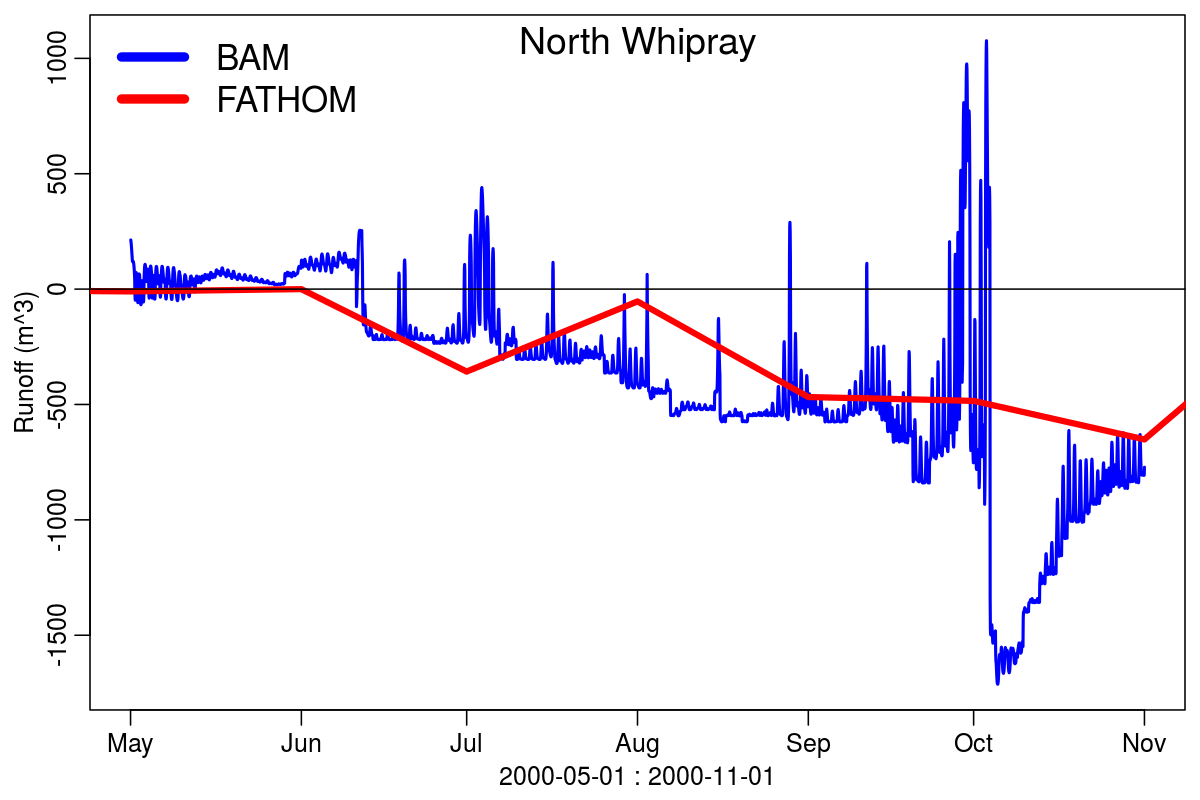
\includegraphics[ width = 0.5\textwidth ]{graphics/RunoffCompare/North Whipray 2000-05-01 Runoff.png}
  }
  \subfloat[2000-05-01]{
    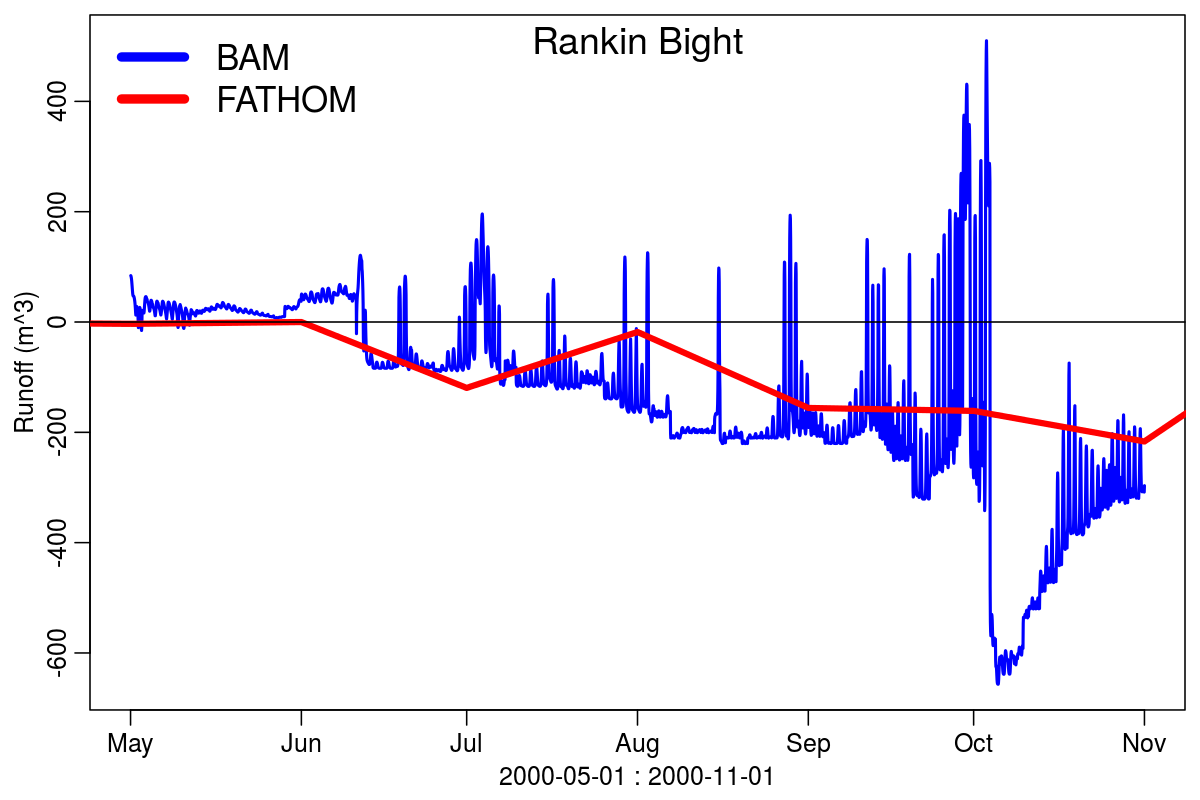
\includegraphics[ width = 0.5\textwidth ]{graphics/RunoffCompare/Rankin Bight 2000-05-01 Runoff.png}
  }
  
  \subfloat[2001-05-01]{
    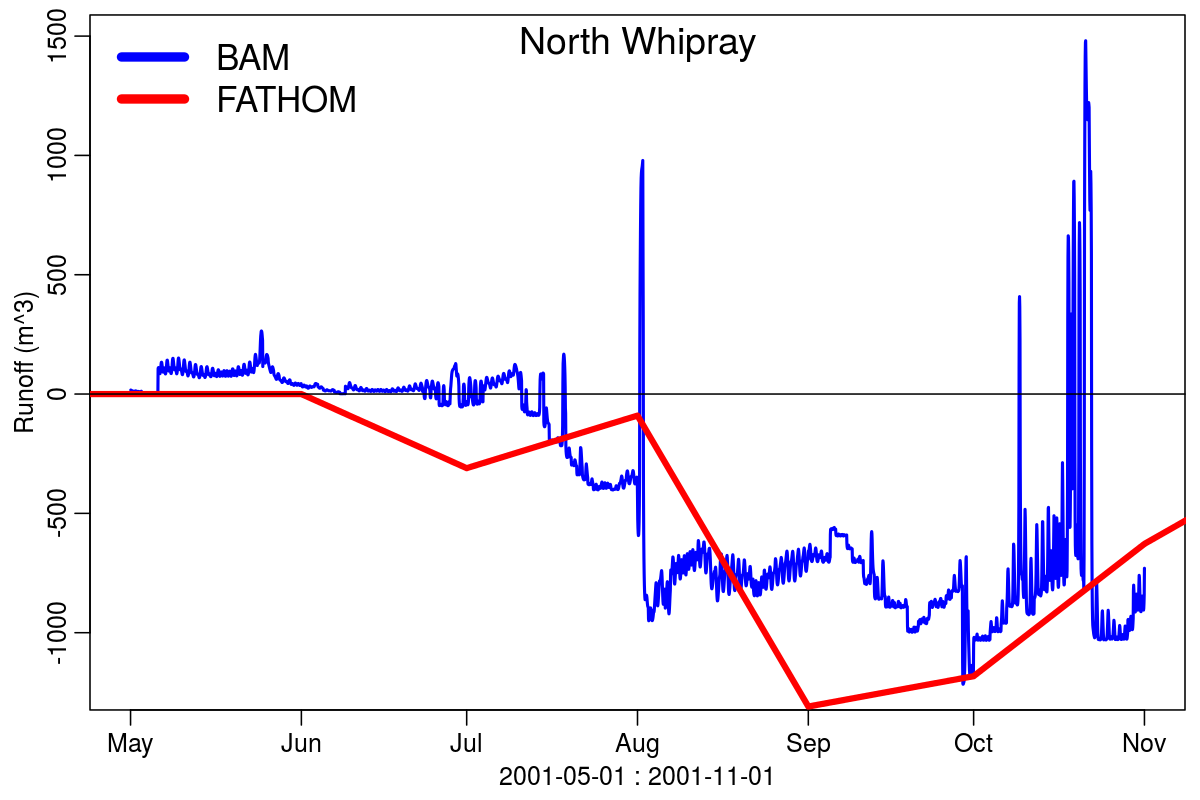
\includegraphics[ width = 0.5\textwidth ]{graphics/RunoffCompare/North Whipray 2001-05-01 Runoff.png}
  }
  \subfloat[2001-05-01]{
    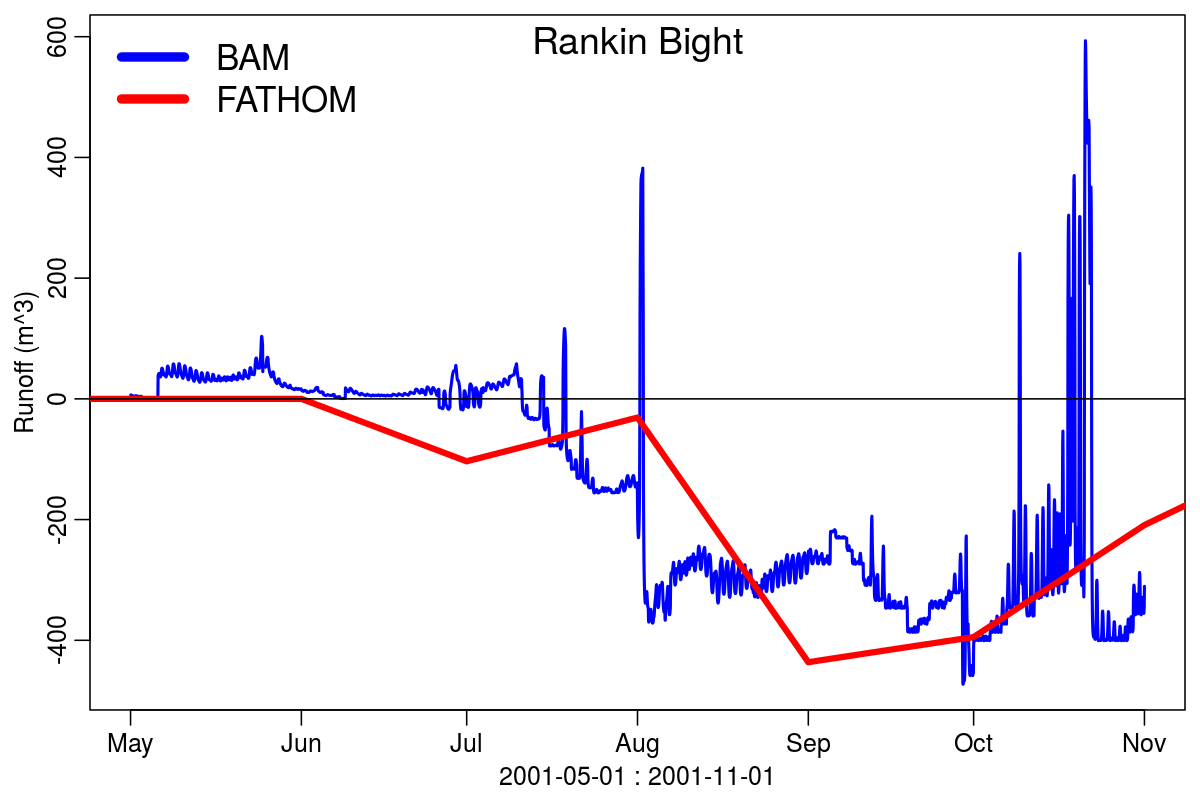
\includegraphics[ width = 0.5\textwidth ]{graphics/RunoffCompare/Rankin Bight 2001-05-01 Runoff.png}
  }

  \subfloat[2002-05-01]{
    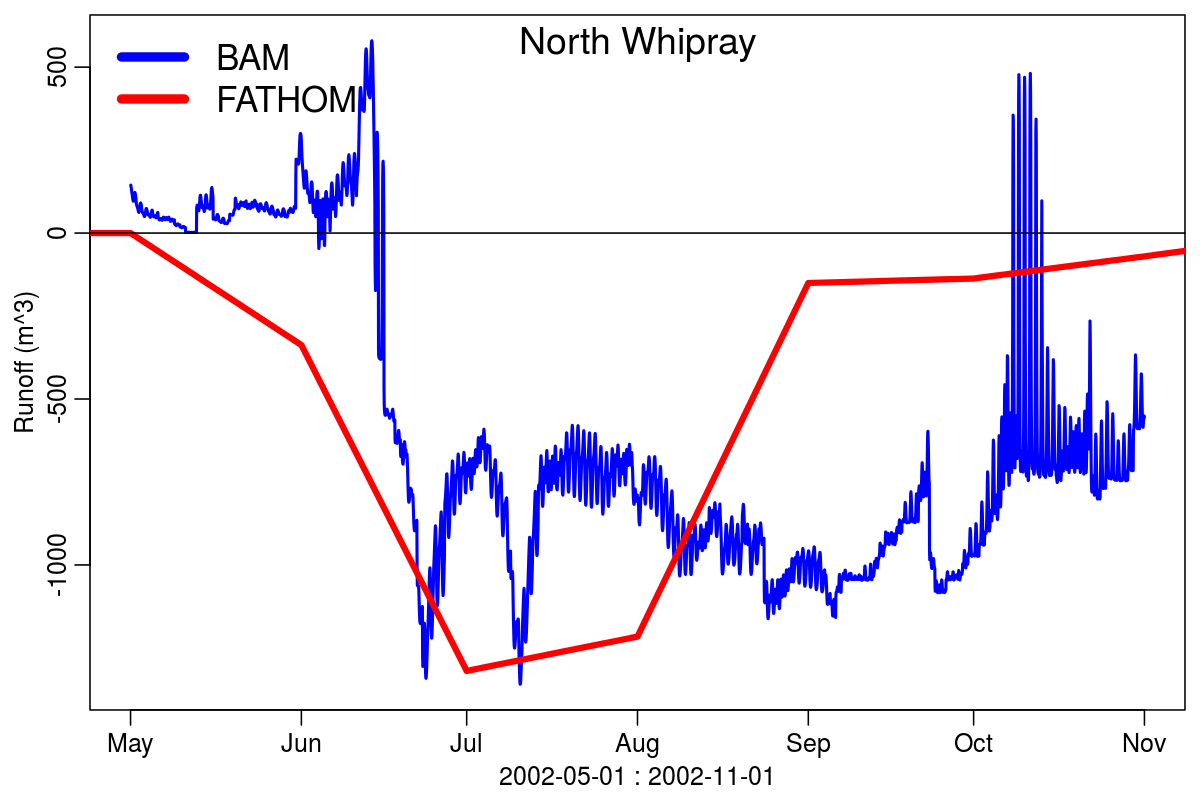
\includegraphics[ width = 0.5\textwidth ]{graphics/RunoffCompare/North Whipray 2002-05-01 Runoff.png}
  }
  \subfloat[2002-05-01]{
    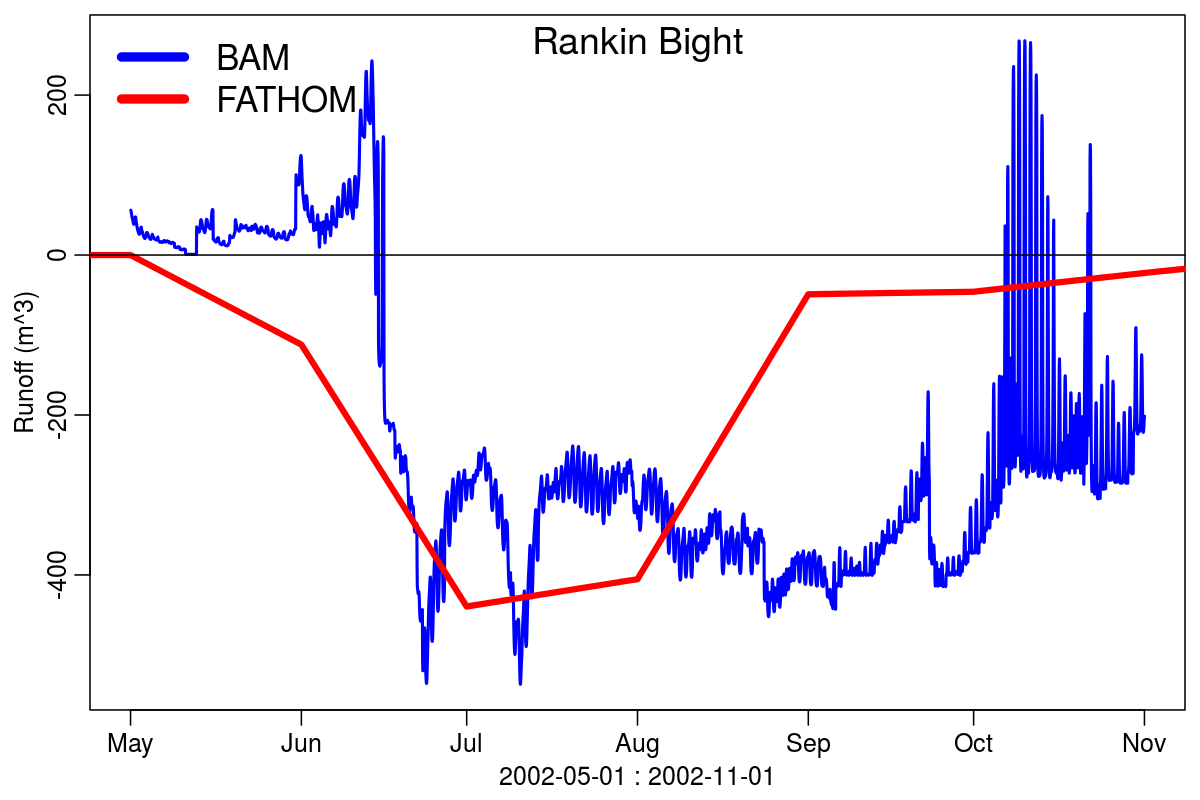
\includegraphics[ width = 0.5\textwidth ]{graphics/RunoffCompare/Rankin Bight 2002-05-01 Runoff.png}
  }
  \caption{North Whipray and Rankin Bight Runoff}
  \label{fig:North Whipray and Rankin Bight Runoff}
\end{figure}
%~~~~~~~~~~~~~~~~~~~~~~~~~~~~~~~~~~~~~~~~~

%~~~~~~~~~~~~~~~~~~~~~~~~~~~~~~~~~~~~~~~~~
\begin{figure}[H]
  \subfloat[2000-05-01]{
    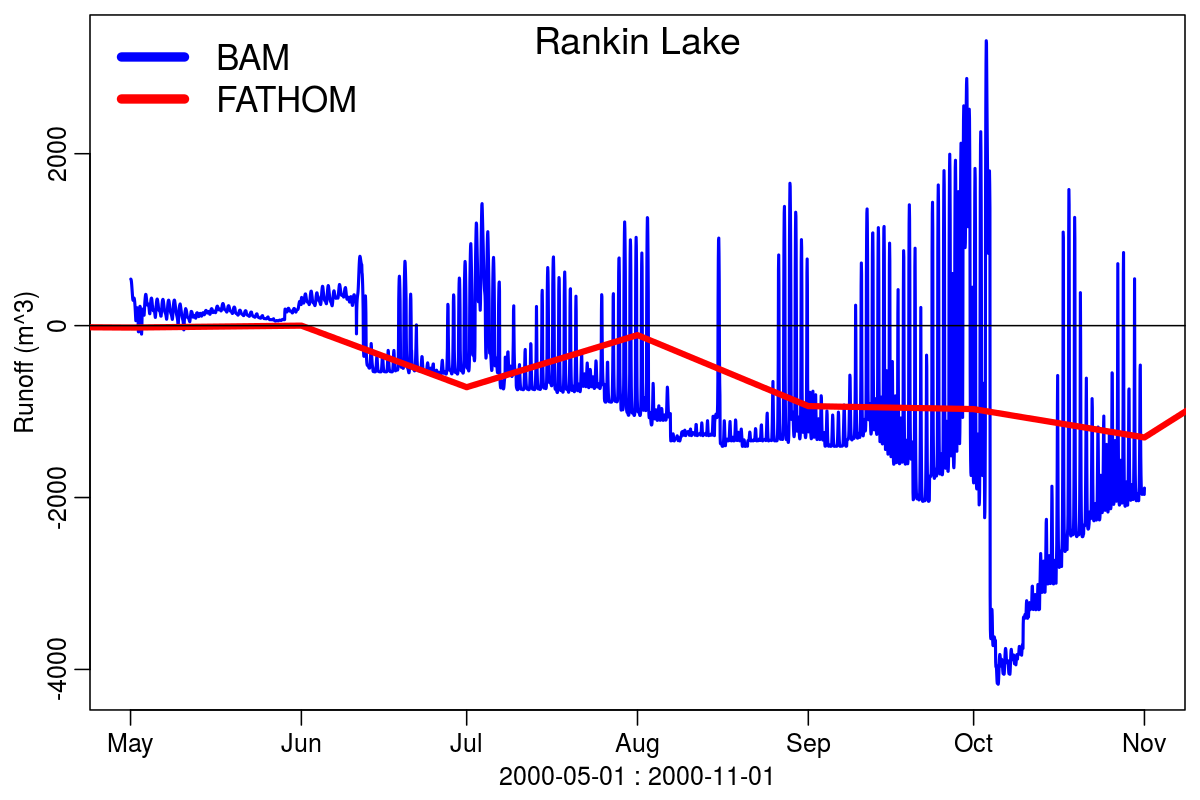
\includegraphics[ width = 0.5\textwidth ]{graphics/RunoffCompare/Rankin Lake 2000-05-01 Runoff.png}
  }
  \subfloat[2000-05-01]{
    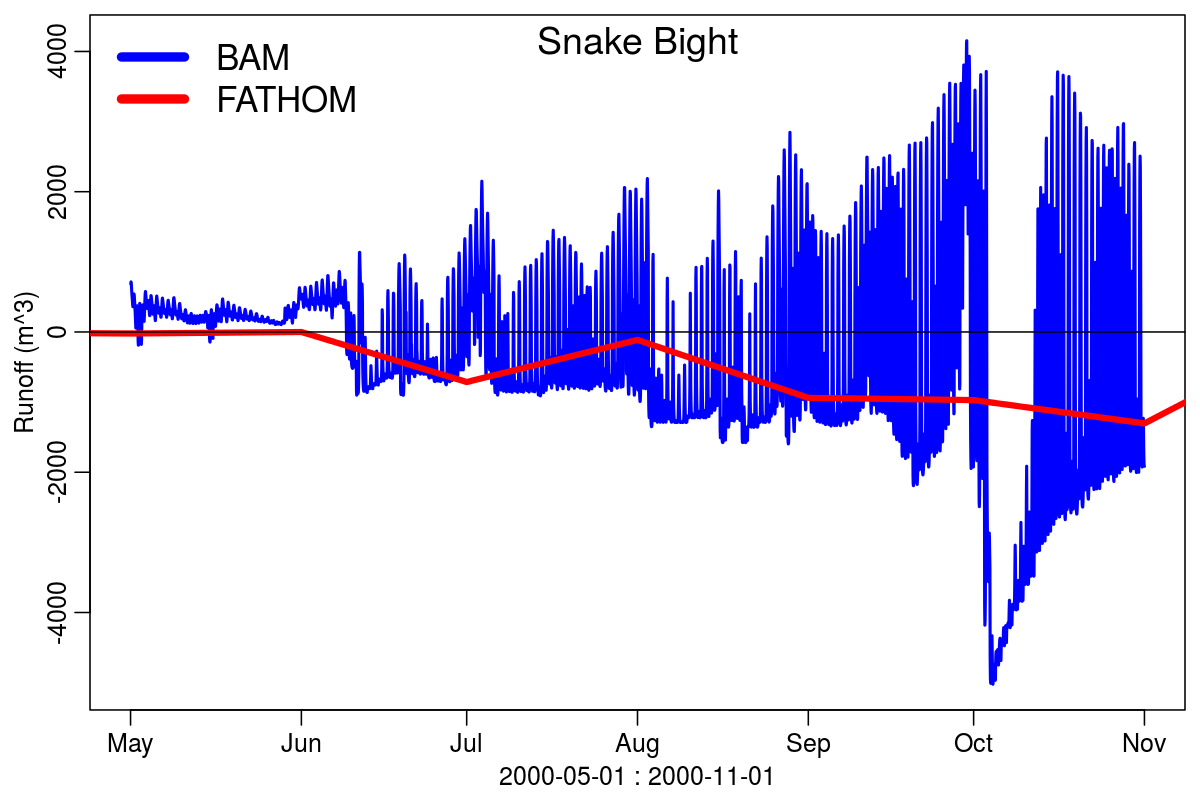
\includegraphics[ width = 0.5\textwidth ]{graphics/RunoffCompare/Snake Bight 2000-05-01 Runoff.png}
  }
  
  \subfloat[2001-05-01]{
    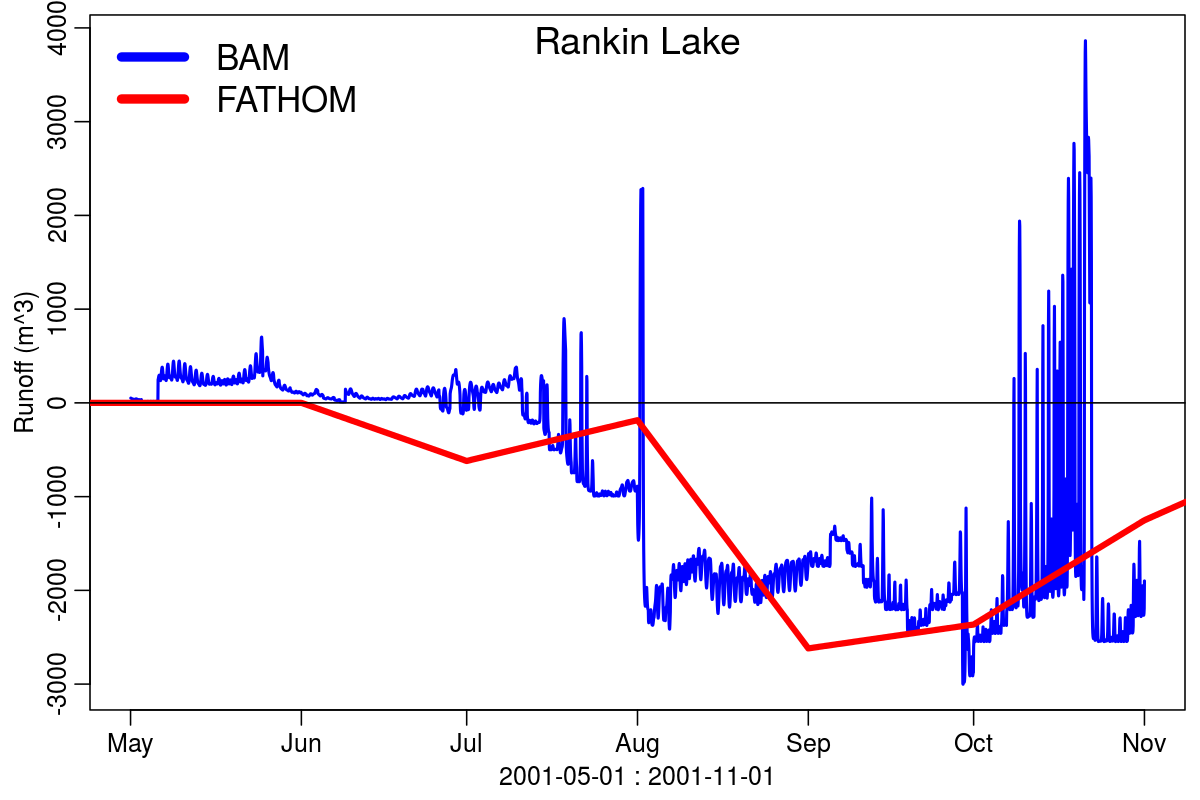
\includegraphics[ width = 0.5\textwidth ]{graphics/RunoffCompare/Rankin Lake 2001-05-01 Runoff.png}
  }
  \subfloat[2001-05-01]{
    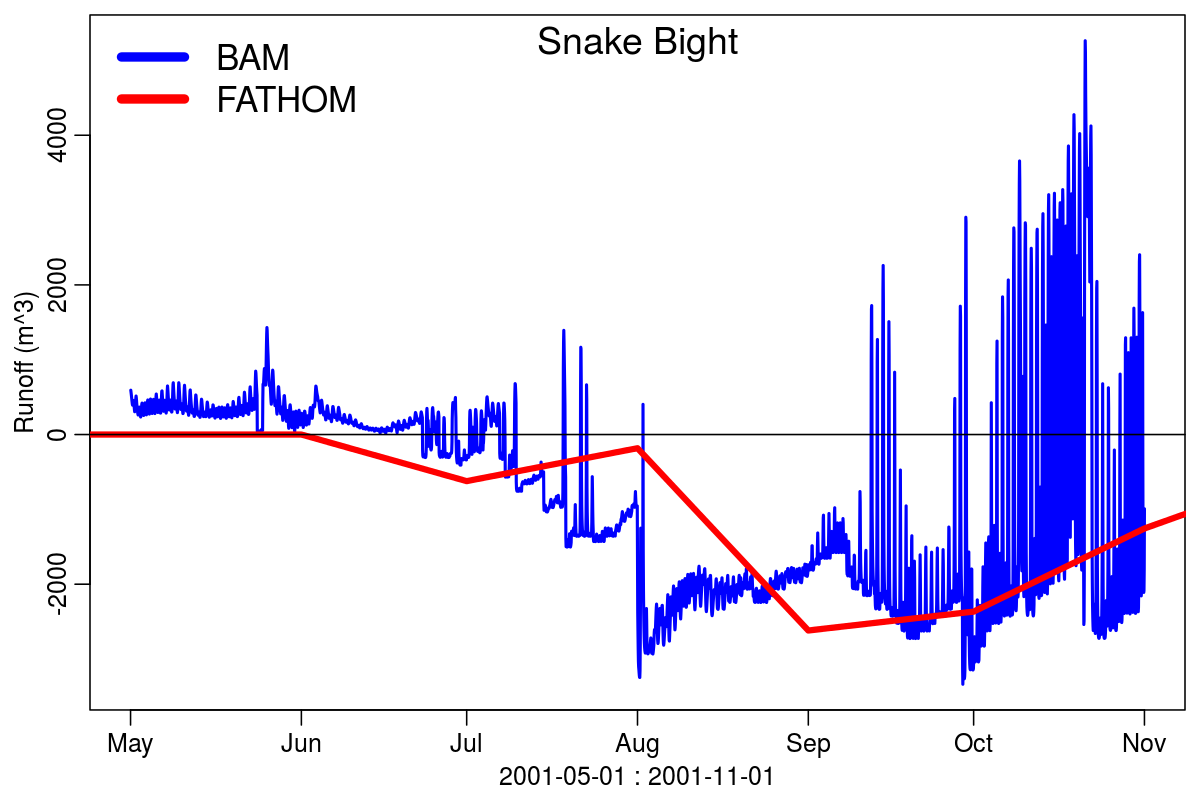
\includegraphics[ width = 0.5\textwidth ]{graphics/RunoffCompare/Snake Bight 2001-05-01 Runoff.png}
  }

  \subfloat[2002-05-01]{
    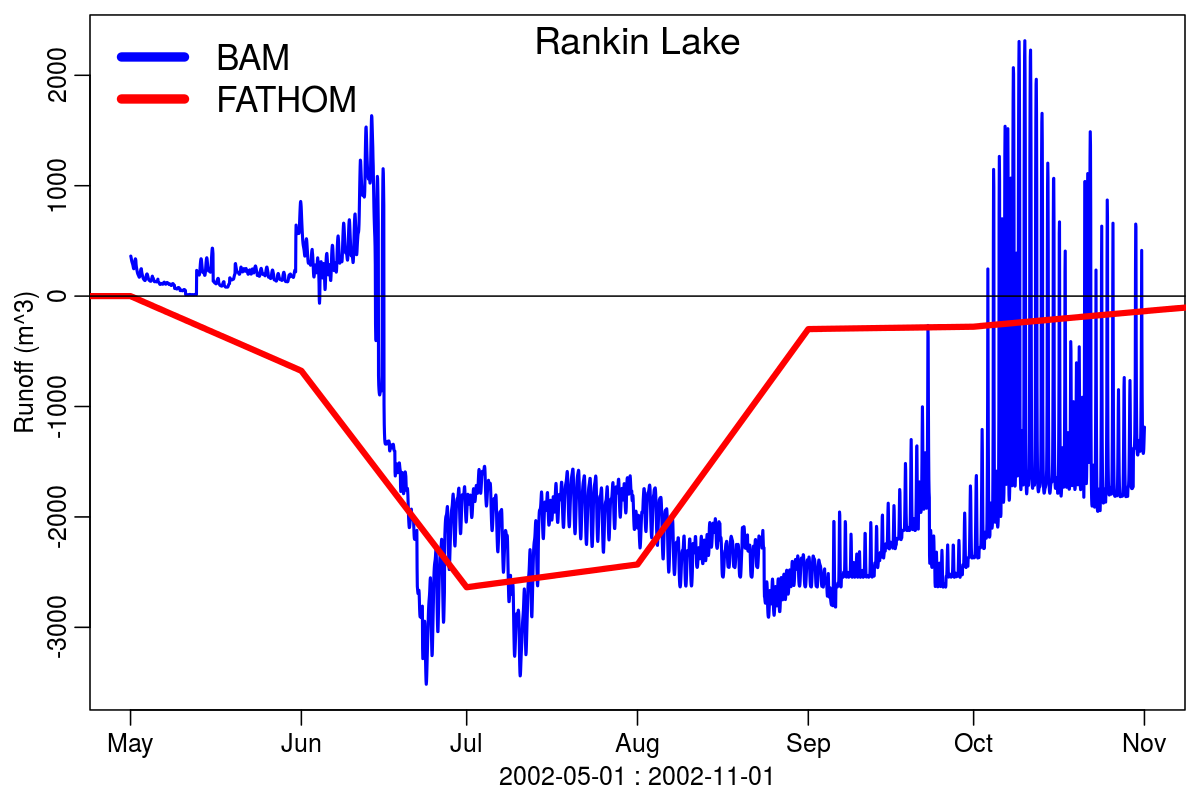
\includegraphics[ width = 0.5\textwidth ]{graphics/RunoffCompare/Rankin Lake 2002-05-01 Runoff.png}
  }
  \subfloat[2002-05-01]{
    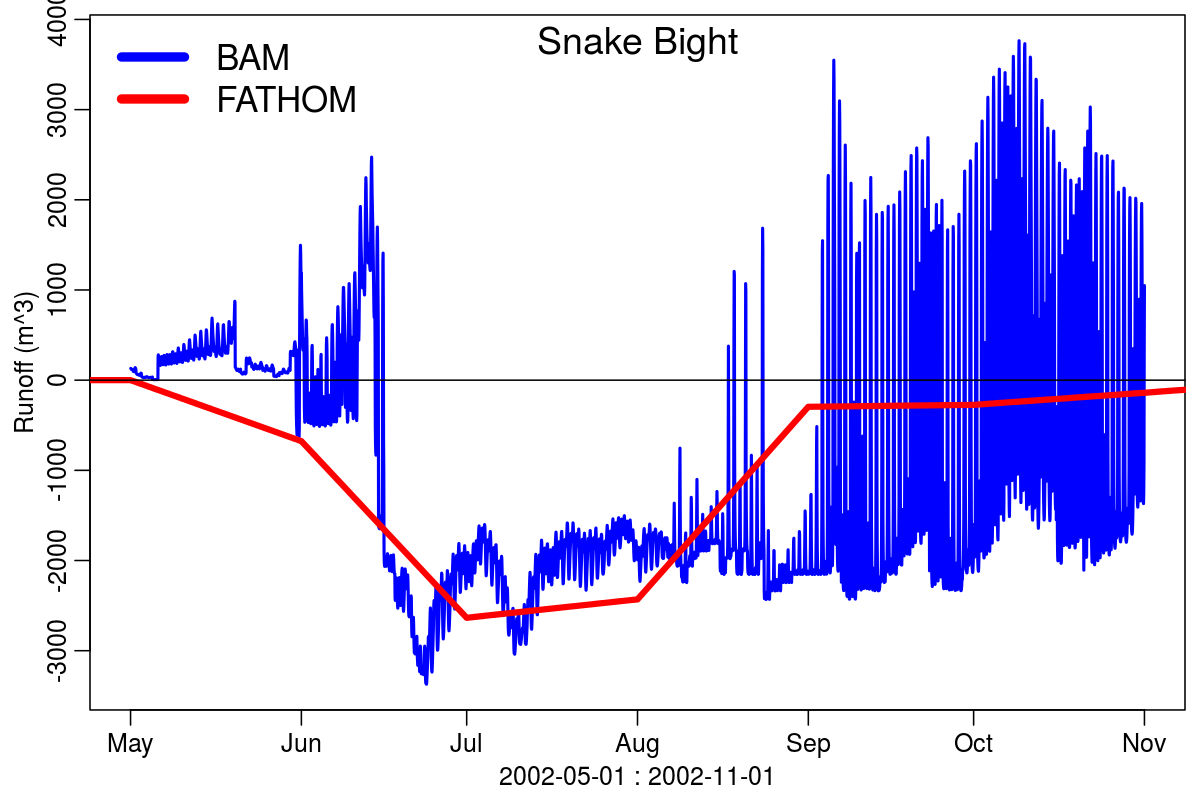
\includegraphics[ width = 0.5\textwidth ]{graphics/RunoffCompare/Snake Bight 2002-05-01 Runoff.png}
  }
  \caption{Rankin Lake and Snake Bight Runoff}
  \label{fig:Rankin Lake and Snake Bight Runoff}
\end{figure}
%~~~~~~~~~~~~~~~~~~~~~~~~~~~~~~~~~~~~~~~~~

%----------------------------------------------------------------
%----------------------------------------------------------------
\clearpage 
\section{Stage Comparison}
\label{sec:Stage Comparison}
%----------------------------------------------------------------
%----------------------------------------------------------------
Interbasin mass transport is driven by hydraulic potential between basins.  Accurate water level simulation is a core competency for good model performance.  This section presents comparisons of basin water levels computed by BAM (blue) and the associated marine monitoring station point-observations (red) over the period 2010-1-1 to 2015-12-1.

%~~~~~~~~~~~~~~~~~~~~~~~~~~~~~~~~~~~~~~~~~
\begin{figure}[H]
  \subfloat[Black Betsy Keys]{
    \includegraphics[ width = 0.45\textwidth ]{graphics/StageCompare/Black Betsy Keys Stage 2010-01-01.png}
  }
  \subfloat[Blackwater Sound]{
    \includegraphics[ width = 0.45\textwidth ]{graphics/StageCompare/Blackwater Sound Stage 2010-01-01.png}
  }

  \subfloat[Butternut Key]{
    \includegraphics[ width = 0.45\textwidth ]{graphics/StageCompare/Butternut Key Stage 2010-01-01.png}
  }
  \subfloat[Deer Key]{
    \includegraphics[ width = 0.45\textwidth ]{graphics/StageCompare/Deer Key Stage 2010-01-01.png}
  }

  \subfloat[Duck Key]{
    \includegraphics[ width = 0.45\textwidth ]{graphics/StageCompare/Duck Key Stage 2010-01-01.png}
  }
  \subfloat[Joe Bay]{
    \includegraphics[ width = 0.45\textwidth ]{graphics/StageCompare/Joe Bay Stage 2010-01-01.png}
  }
  \caption{Water level comparisons: Black Betsy Keys, Blackwater Sound, Butternut Key, Deer Key, Duck Key and Joe Bay.}
  \label{fig:Stage compare 1}
\end{figure}
%~~~~~~~~~~~~~~~~~~~~~~~~~~~~~~~~~~~~~~~~~

%~~~~~~~~~~~~~~~~~~~~~~~~~~~~~~~~~~~~~~~~~
\begin{figure}[H]
  \subfloat[Johnson Key]{
    \includegraphics[ width = 0.5\textwidth ]{graphics/StageCompare/Johnson Key Stage 2010-01-01.png}
  }
  \subfloat[Lignumvitae]{
    \includegraphics[ width = 0.5\textwidth ]{graphics/StageCompare/Lignumvitae Stage 2010-01-01.png}
  }

  \subfloat[Little Blackwater Sound]{
    \includegraphics[ width = 0.5\textwidth ]{graphics/StageCompare/Little Blackwater Sound Stage 2010-01-01.png}
  }
  \subfloat[Little Madeira Bay]{
    \includegraphics[ width = 0.5\textwidth ]{graphics/StageCompare/Little Madeira Bay Stage 2010-01-01.png}
  }

  \subfloat[Long Key]{
    \includegraphics[ width = 0.5\textwidth ]{graphics/StageCompare/Long Key Stage 2010-01-01.png}
  }
  \subfloat[Long Sound]{
    \includegraphics[ width = 0.5\textwidth ]{graphics/StageCompare/Long Sound Stage 2010-01-01.png}
  }
  \caption{Water level comparisons: Johnson Key, Lignumvitae, Little Blackwater Sound, Little Madeira Bay, Long Key and Long Sound.}
  \label{fig:Stage compare 2}
\end{figure}
%~~~~~~~~~~~~~~~~~~~~~~~~~~~~~~~~~~~~~~~~~

%~~~~~~~~~~~~~~~~~~~~~~~~~~~~~~~~~~~~~~~~~
\begin{figure}[H]
  \subfloat[Manatee Bay]{
    \includegraphics[ width = 0.5\textwidth ]{graphics/StageCompare/Manatee Bay Stage 2010-01-01.png}
  }
  \subfloat[Porpoise Lake]{
    \includegraphics[ width = 0.5\textwidth ]{graphics/StageCompare/Porpoise Lake Stage 2010-01-01.png}
  }

  \subfloat[Rankin Lake]{
    \includegraphics[ width = 0.5\textwidth ]{graphics/StageCompare/Rankin Lake Stage 2010-01-01.png}
  }
  \subfloat[Snake Bight]{
    \includegraphics[ width = 0.5\textwidth ]{graphics/StageCompare/Snake Bight Stage 2010-01-01.png}
  }

  \subfloat[Twin Keys]{
    \includegraphics[ width = 0.5\textwidth ]{graphics/StageCompare/Twin Keys Stage 2010-01-01.png}
  }
  \subfloat[Whipray]{
    \includegraphics[ width = 0.5\textwidth ]{graphics/StageCompare/Whipray Stage 2010-01-01.png}
  }
  \caption{Water level comparisons: Manatee Bay, Porpoise Lake, Rankin Lake, Snake Bight, Twin Keys and Whipray.}
  \label{fig:Stage compare 3}
\end{figure}
%~~~~~~~~~~~~~~~~~~~~~~~~~~~~~~~~~~~~~~~~~


%----------------------------------------------------------------
%----------------------------------------------------------------
\clearpage 
\section{Salinity Comparison}
\label{sec:Salinity Comparison}
%----------------------------------------------------------------
%----------------------------------------------------------------
Salinity comparisons for the period 1999-9-1 to 2015-12-7 are shown in figure \ref{fig:Salinity Compare 1999-2015}. Top panel is BAM output, bottom panel observed data.
%~~~~~~~~~~~~~~~~~~~~~~~~~~~~~~~~~~~~~~~~~
\begin{figure}[H]
  \subfloat[NE Basins]{
    \includegraphics[ width = 0.46\textwidth ]{graphics/SalinityCompare/1999_2015/NE_Salinity_1999-9-1_2015-12-7.png}
  }
  \subfloat[Central Basins]{
    \includegraphics[ width = 0.47\textwidth ]{graphics/SalinityCompare/1999_2015/Central_Salinity_1999-9-1_2015-12-7.png}
  }
  
  \subfloat[Central SE Basins]{
    \includegraphics[ width = 0.43\textwidth ]{graphics/SalinityCompare/1999_2015/Central_SE_Salinity_1999-9-1_2015-12-7.png}
  }
  \subfloat[Rankin Lake]{
    \includegraphics[ width = 0.45\textwidth ]{graphics/SalinityCompare/1999_2015/RankinLake_Salinity_1999-9-1_2015-12-7.png}
  }
  \caption{Salinity comparisons 1999-9-1 to 2015-12-7.}
  \label{fig:Salinity Compare 1999-2015}
\end{figure}
%~~~~~~~~~~~~~~~~~~~~~~~~~~~~~~~~~~~~~~~~~

Salinity comparisons for the period 2010-1-1 to 2015-12-7 are shown in figure \ref{fig:Salinity Compare 1999-2015}. Top panel is BAM output, bottom panel observed data.
%~~~~~~~~~~~~~~~~~~~~~~~~~~~~~~~~~~~~~~~~~
\begin{figure}[H]
  \subfloat[NE Basins]{
    \includegraphics[ width = 0.72\textwidth ]{graphics/SalinityCompare/2010_2015/BAM_2010_2015_Salinity_NE.png}
  }

  \subfloat[N Basins]{
    \includegraphics[ width = 0.72\textwidth ]{graphics/SalinityCompare/2010_2015/BAM_2010_2015_Salinity_N.png}
  }
  \caption{Salinity comparisons 2010-1-1 to 2015-12-7.}
  \label{fig:Salinity Compare 2010-2015}
\end{figure}
%~~~~~~~~~~~~~~~~~~~~~~~~~~~~~~~~~~~~~~~~~

%~~~~~~~~~~~~~~~~~~~~~~~~~~~~~~~~~~~~~~~~~
\begin{figure}[H]
  \subfloat[NW Basins]{
    \includegraphics[ width = 0.8\textwidth ]{graphics/SalinityCompare/2010_2015/BAM_2010_2015_Salinity_NW.png}
  }
  \caption{Salinity comparisons 2010-1-1 to 2015-12-7.}
  \label{fig:NW Salinity Compare 2010-2015}
\end{figure}
%~~~~~~~~~~~~~~~~~~~~~~~~~~~~~~~~~~~~~~~~~

\clearpage
Salinity comparisons over the rainy seasons of 2000, 2001, and 2002 are shown below. Top panels are BAM output, bottom panels observed salinity. BAM values are basin-wide, observations are point measurements, and not necessarily in the same basin as the BAM output. In some cases multiple observations from adjacent basins are shown. 
%~~~~~~~~~~~~~~~~~~~~~~~~~~~~~~~~~~~~~~~~~
\begin{figure}[H]
  \subfloat[Barnes Sound 2000]{
    \includegraphics[ width = 0.5\textwidth ]{graphics/SalinityCompare/2000_2002/Barnes Sound 2000-5-1 Salinity.png}
  }
  \subfloat[Black Betsy Key 2000]{
    \includegraphics[ width = 0.5\textwidth ]{graphics/SalinityCompare/2000_2002/Black Betsy Keys 2000-5-1 Salinity.png}
  }

  \subfloat[Barnes Sound 2001]{
    \includegraphics[ width = 0.5\textwidth ]{graphics/SalinityCompare/2000_2002/Barnes Sound 2001-5-1 Salinity.png}
  }
  \subfloat[Black Betsy Key 2001]{
    \includegraphics[ width = 0.5\textwidth ]{graphics/SalinityCompare/2000_2002/Black Betsy Keys 2001-5-1 Salinity.png}
  }

  \subfloat[Barnes Sound 2001]{
    \includegraphics[ width = 0.5\textwidth ]{graphics/SalinityCompare/2000_2002/Barnes Sound 2002-5-1 Salinity.png}
  }
  \subfloat[Black Betsy Key 2002]{
    \includegraphics[ width = 0.5\textwidth ]{graphics/SalinityCompare/2000_2002/Black Betsy Keys 2002-5-1 Salinity.png}
  }

  \caption{Salinity comparisons at Barnes Sound and Black Betsy Key 2000-2002.}
  \label{fig:Salinity Compare 2000-2002 1}
\end{figure}
%~~~~~~~~~~~~~~~~~~~~~~~~~~~~~~~~~~~~~~~~~


%~~~~~~~~~~~~~~~~~~~~~~~~~~~~~~~~~~~~~~~~~
\begin{figure}[H]
  \subfloat[Blackwater Sound 2000]{
    \includegraphics[ width = 0.5\textwidth ]{graphics/SalinityCompare/2000_2002/Blackwater Sound 2000-5-1 Salinity.png}
  }
  \subfloat[Butternut Key 2000]{
    \includegraphics[ width = 0.5\textwidth ]{graphics/SalinityCompare/2000_2002/Butternut Key 2000-5-1 Salinity.png}
  }

  \subfloat[Blackwater Sound 2001]{
    \includegraphics[ width = 0.5\textwidth ]{graphics/SalinityCompare/2000_2002/Blackwater Sound 2001-5-1 Salinity.png}
  }
  \subfloat[Butternut Key 2001]{
    \includegraphics[ width = 0.5\textwidth ]{graphics/SalinityCompare/2000_2002/Butternut Key 2001-5-1 Salinity.png}
  }

  \subfloat[Blackwater Sound 2002]{
    \includegraphics[ width = 0.5\textwidth ]{graphics/SalinityCompare/2000_2002/Blackwater Sound 2002-5-1 Salinity.png}
  }
  \subfloat[Butternut Key 2002]{
    \includegraphics[ width = 0.5\textwidth ]{graphics/SalinityCompare/2000_2002/Butternut Key 2002-5-1 Salinity.png}
  }

  \caption{Salinity comparisons at Blackwater Sound, and Butternut Key 2000-2002.}
  \label{fig:Salinity Compare 2000-2002 2}
\end{figure}
%~~~~~~~~~~~~~~~~~~~~~~~~~~~~~~~~~~~~~~~~~


%~~~~~~~~~~~~~~~~~~~~~~~~~~~~~~~~~~~~~~~~~
\begin{figure}[H]
  \subfloat[Catfish Key 2000]{
    \includegraphics[ width = 0.5\textwidth ]{graphics/SalinityCompare/2000_2002/Catfish Key 2000-5-1 Salinity.png}
  }
  \subfloat[Deer Key 2000]{
    \includegraphics[ width = 0.5\textwidth ]{graphics/SalinityCompare/2000_2002/Deer Key 2000-5-1 Salinity.png}
  }

  \subfloat[Catfish Key 2001]{
    \includegraphics[ width = 0.5\textwidth ]{graphics/SalinityCompare/2000_2002/Catfish Key 2001-5-1 Salinity.png}
  }
  \subfloat[Deer Key 2001]{
    \includegraphics[ width = 0.5\textwidth ]{graphics/SalinityCompare/2000_2002/Deer Key 2001-5-1 Salinity.png}
  }

  \subfloat[Catfish Key 2002]{
    \includegraphics[ width = 0.5\textwidth ]{graphics/SalinityCompare/2000_2002/Catfish Key 2002-5-1 Salinity.png}
  }
  \subfloat[Deer Key 2002]{
    \includegraphics[ width = 0.5\textwidth ]{graphics/SalinityCompare/2000_2002/Deer Key 2002-5-1 Salinity.png}
  }

  \caption{Salinity comparisons at Catfish Key and Deer Key 2000-2002.}
  \label{fig:Salinity Compare 2000-2002 3}
\end{figure}
%~~~~~~~~~~~~~~~~~~~~~~~~~~~~~~~~~~~~~~~~~


%~~~~~~~~~~~~~~~~~~~~~~~~~~~~~~~~~~~~~~~~~
\begin{figure}[H]
  \subfloat[Duck Key 2000]{
    \includegraphics[ width = 0.5\textwidth ]{graphics/SalinityCompare/2000_2002/Duck Key 2000-5-1 Salinity.png}
  }
  \subfloat[Joe Bay 2000]{
    \includegraphics[ width = 0.5\textwidth ]{graphics/SalinityCompare/2000_2002/Joe Bay 2000-5-1 Salinity.png}
  }

  \subfloat[Duck Key 2001]{
    \includegraphics[ width = 0.5\textwidth ]{graphics/SalinityCompare/2000_2002/Duck Key 2001-5-1 Salinity.png}
  }
  \subfloat[Joe Bay 2001]{
    \includegraphics[ width = 0.5\textwidth ]{graphics/SalinityCompare/2000_2002/Joe Bay 2001-5-1 Salinity.png}
  }

  \subfloat[Duck Key 2002]{
    \includegraphics[ width = 0.5\textwidth ]{graphics/SalinityCompare/2000_2002/Duck Key 2002-5-1 Salinity.png}
  }
  \subfloat[Joe Bay 2002]{
    \includegraphics[ width = 0.5\textwidth ]{graphics/SalinityCompare/2000_2002/Joe Bay 2002-5-1 Salinity.png}
  }

  \caption{Salinity comparisons at Duck Key and Joe Bay 2000-2002.}
  \label{fig:Salinity Compare 2000-2002 4}
\end{figure}
%~~~~~~~~~~~~~~~~~~~~~~~~~~~~~~~~~~~~~~~~~


%~~~~~~~~~~~~~~~~~~~~~~~~~~~~~~~~~~~~~~~~~
\begin{figure}[H]
  \subfloat[Johnson Key 2000]{
    \includegraphics[ width = 0.5\textwidth ]{graphics/SalinityCompare/2000_2002/Johnson Key 2000-5-1 Salinity.png}
  }
  \subfloat[Lignumvitae 2000]{
    \includegraphics[ width = 0.5\textwidth ]{graphics/SalinityCompare/2000_2002/Lignumvitae 2000-5-1 Salinity.png}
  }

  \subfloat[Johnson Key 2001]{
    \includegraphics[ width = 0.5\textwidth ]{graphics/SalinityCompare/2000_2002/Johnson Key 2001-5-1 Salinity.png}
  }
  \subfloat[Lignumvitae 2001]{
    \includegraphics[ width = 0.5\textwidth ]{graphics/SalinityCompare/2000_2002/Lignumvitae 2001-5-1 Salinity.png}
  }

  \subfloat[Johnson Key 2002]{
    \includegraphics[ width = 0.5\textwidth ]{graphics/SalinityCompare/2000_2002/Johnson Key 2002-5-1 Salinity.png}
  }
  \subfloat[Lignumvitae 2002]{
    \includegraphics[ width = 0.5\textwidth ]{graphics/SalinityCompare/2000_2002/Lignumvitae 2002-5-1 Salinity.png}
  }

  \caption{Salinity comparisons at Johnson Key and Lignumvitae 2000-2002.}
  \label{fig:Salinity Compare 2000-2002 5}
\end{figure}
%~~~~~~~~~~~~~~~~~~~~~~~~~~~~~~~~~~~~~~~~~


%~~~~~~~~~~~~~~~~~~~~~~~~~~~~~~~~~~~~~~~~~
\begin{figure}[H]
  \subfloat[Little Blackwater Sound 2000]{
    \includegraphics[ width = 0.5\textwidth ]{graphics/SalinityCompare/2000_2002/Little Blackwater Sound 2000-5-1 Salinity.png}
  }
  \subfloat[Little Madeira Bay 2000]{
    \includegraphics[ width = 0.5\textwidth ]{graphics/SalinityCompare/2000_2002/Little Madeira Bay 2000-5-1 Salinity.png}
  }

  \subfloat[Little Blackwater Sound 2001]{
    \includegraphics[ width = 0.5\textwidth ]{graphics/SalinityCompare/2000_2002/Little Blackwater Sound 2001-5-1 Salinity.png}
  }
  \subfloat[Little Madeira Bay 2001]{
    \includegraphics[ width = 0.5\textwidth ]{graphics/SalinityCompare/2000_2002/Little Madeira Bay 2001-5-1 Salinity.png}
  }

  \subfloat[Little Blackwater Sound 2002]{
    \includegraphics[ width = 0.5\textwidth ]{graphics/SalinityCompare/2000_2002/Little Blackwater Sound 2002-5-1 Salinity.png}
  }
  \subfloat[Little Madeira Bay 2002]{
    \includegraphics[ width = 0.5\textwidth ]{graphics/SalinityCompare/2000_2002/Little Madeira Bay 2002-5-1 Salinity.png}
  }

  \caption{Salinity comparisons at Little Blackwater Sound and Little Madeira Bay 2000-2002.}
  \label{fig:Salinity Compare 2000-2002 6}
\end{figure}
%~~~~~~~~~~~~~~~~~~~~~~~~~~~~~~~~~~~~~~~~~


%~~~~~~~~~~~~~~~~~~~~~~~~~~~~~~~~~~~~~~~~~
\begin{figure}[H]
  \subfloat[Long Sound 2000]{
    \includegraphics[ width = 0.5\textwidth ]{graphics/SalinityCompare/2000_2002/Long Sound 2000-5-1 Salinity.png}
  }
  \subfloat[Manatee Bay 2000]{
    \includegraphics[ width = 0.5\textwidth ]{graphics/SalinityCompare/2000_2002/Manatee Bay 2000-5-1 Salinity.png}
  }

  \subfloat[Long Sound 2001]{
    \includegraphics[ width = 0.5\textwidth ]{graphics/SalinityCompare/2000_2002/Long Sound 2001-5-1 Salinity.png}
  }
  \subfloat[Manatee Bay 2001]{
    \includegraphics[ width = 0.5\textwidth ]{graphics/SalinityCompare/2000_2002/Manatee Bay 2001-5-1 Salinity.png}
  }

  \subfloat[Long Sound 2002]{
    \includegraphics[ width = 0.5\textwidth ]{graphics/SalinityCompare/2000_2002/Long Sound 2002-5-1 Salinity.png}
  }
  \subfloat[Manatee Bay 2002]{
    \includegraphics[ width = 0.5\textwidth ]{graphics/SalinityCompare/2000_2002/Manatee Bay 2002-5-1 Salinity.png}
  }

  \caption{Salinity comparisons at Long Sound and Manatee Bay 2000-2002.}
  \label{fig:Salinity Compare 2000-2002 7}
\end{figure}
%~~~~~~~~~~~~~~~~~~~~~~~~~~~~~~~~~~~~~~~~~


%~~~~~~~~~~~~~~~~~~~~~~~~~~~~~~~~~~~~~~~~~
\begin{figure}[H]
  \subfloat[Porpoise Lake 2000]{
    \includegraphics[ width = 0.5\textwidth ]{graphics/SalinityCompare/2000_2002/Porpoise Lake 2000-5-1 Salinity.png}
  }
  \subfloat[Rabbit Key 2000]{
    \includegraphics[ width = 0.5\textwidth ]{graphics/SalinityCompare/2000_2002/Rabbit Key 2000-5-1 Salinity.png}
  }

  \subfloat[Porpoise Lake 2001]{
    \includegraphics[ width = 0.5\textwidth ]{graphics/SalinityCompare/2000_2002/Porpoise Lake 2001-5-1 Salinity.png}
  }
  \subfloat[Rabbit Key 2001]{
    \includegraphics[ width = 0.5\textwidth ]{graphics/SalinityCompare/2000_2002/Rabbit Key 2001-5-1 Salinity.png}
  }

  \subfloat[Porpoise Lake 2002]{
    \includegraphics[ width = 0.5\textwidth ]{graphics/SalinityCompare/2000_2002/Porpoise Lake 2002-5-1 Salinity.png}
  }
  \subfloat[Rabbit Key 2002]{
    \includegraphics[ width = 0.5\textwidth ]{graphics/SalinityCompare/2000_2002/Rabbit Key 2002-5-1 Salinity.png}
  }

  \caption{Salinity comparisons at Porpoise Lake and Rabbit Key 2000-2002.}
  \label{fig:Salinity Compare 2000-2002 8}
\end{figure}
%~~~~~~~~~~~~~~~~~~~~~~~~~~~~~~~~~~~~~~~~~


%~~~~~~~~~~~~~~~~~~~~~~~~~~~~~~~~~~~~~~~~~
\begin{figure}[H]
  \subfloat[Rankin Lake 2000]{
    \includegraphics[ width = 0.5\textwidth ]{graphics/SalinityCompare/2000_2002/Rankin Lake 2000-5-1 Salinity.png}
  }
  \subfloat[Snake Bight 2000]{
    \includegraphics[ width = 0.5\textwidth ]{graphics/SalinityCompare/2000_2002/Snake Bight 2000-5-1 Salinity.png}
  }

  \subfloat[Rankin Lake 2001]{
    \includegraphics[ width = 0.5\textwidth ]{graphics/SalinityCompare/2000_2002/Rankin Lake 2001-5-1 Salinity.png}
  }
  \subfloat[Snake Bight 2001]{
    \includegraphics[ width = 0.5\textwidth ]{graphics/SalinityCompare/2000_2002/Snake Bight 2001-5-1 Salinity.png}
  }

  \subfloat[Rankin Lake 2002]{
    \includegraphics[ width = 0.5\textwidth ]{graphics/SalinityCompare/2000_2002/Rankin Lake 2002-5-1 Salinity.png}
  }
  \subfloat[Snake Bight 2002]{
    \includegraphics[ width = 0.5\textwidth ]{graphics/SalinityCompare/2000_2002/Snake Bight 2002-5-1 Salinity.png}
  }

  \caption{Salinity comparisons at Rankin Lake and Snake Bight 2000-2002.}
  \label{fig:Salinity Compare 2000-2002 9}
\end{figure}
%~~~~~~~~~~~~~~~~~~~~~~~~~~~~~~~~~~~~~~~~~


%~~~~~~~~~~~~~~~~~~~~~~~~~~~~~~~~~~~~~~~~~
\begin{figure}[H]
  \subfloat[Swash Keys 2000]{
    \includegraphics[ width = 0.5\textwidth ]{graphics/SalinityCompare/2000_2002/Swash Keys 2000-5-1 Salinity.png}
  }
  \subfloat[Twin Keys 2000]{
    \includegraphics[ width = 0.5\textwidth ]{graphics/SalinityCompare/2000_2002/Twin Keys 2000-5-1 Salinity.png}
  }

  \subfloat[Swash Keys 2001]{
    \includegraphics[ width = 0.5\textwidth ]{graphics/SalinityCompare/2000_2002/Swash Keys 2001-5-1 Salinity.png}
  }
  \subfloat[Twin Keys 2001]{
    \includegraphics[ width = 0.5\textwidth ]{graphics/SalinityCompare/2000_2002/Twin Keys 2001-5-1 Salinity.png}
  }

  \subfloat[Swash Keys 2002]{
    \includegraphics[ width = 0.5\textwidth ]{graphics/SalinityCompare/2000_2002/Swash Keys 2002-5-1 Salinity.png}
  }
  \subfloat[Twin Keys 2002]{
    \includegraphics[ width = 0.5\textwidth ]{graphics/SalinityCompare/2000_2002/Twin Keys 2002-5-1 Salinity.png}
  }

  \caption{Salinity comparisons at Swash Keys and Twin Keys 2000-2002.}
  \label{fig:Salinity Compare 2000-2002 10}
\end{figure}
%~~~~~~~~~~~~~~~~~~~~~~~~~~~~~~~~~~~~~~~~~


%~~~~~~~~~~~~~~~~~~~~~~~~~~~~~~~~~~~~~~~~~
\begin{figure}[H]
  \subfloat[Whipray 2000]{
    \includegraphics[ width = 0.5\textwidth ]{graphics/SalinityCompare/2000_2002/Whipray 2000-5-1 Salinity.png}
  }

  \subfloat[Whipray 2001]{
    \includegraphics[ width = 0.5\textwidth ]{graphics/SalinityCompare/2000_2002/Whipray 2001-5-1 Salinity.png}
  }

  \subfloat[Whipray 2002]{
    \includegraphics[ width = 0.5\textwidth ]{graphics/SalinityCompare/2000_2002/Whipray 2002-5-1 Salinity.png}
  }

  \caption{Salinity comparisons at Whipray 2000-2002.}
  \label{fig:Salinity Compare 2000-2002 11}
\end{figure}
%~~~~~~~~~~~~~~~~~~~~~~~~~~~~~~~~~~~~~~~~~


\cleardoublepage
